\documentclass[a4paper,12pt]{article}
% Package to make citations superscrit with brackets
\usepackage[super,square]{natbib}
% Package to change margin size
\usepackage{anysize}
\marginsize{2cm}{2cm}{1cm}{2cm}
% Package to make headers
\usepackage{fancyhdr}
\renewcommand{\headrulewidth}{0pt}
% Package for highligths
\usepackage{soul}
% Colors for the references links
\usepackage[dvipsnames]{xcolor}
% Package to link references
\usepackage{hyperref}
\usepackage{graphicx}
\usepackage{float}
\usepackage[italian]{babel}
\hypersetup{
    colorlinks=true,
    linkcolor=black,
    citecolor=CadetBlue,
    filecolor=CadetBlue,      
    urlcolor=CadetBlue,
}
% Package for lorem ipsum
\usepackage{lipsum}
% Package for multicolumn
\usepackage{multicol}
\usepackage{amsmath}
\usepackage{multicol,caption}
% Package for removing paragraph identations
\usepackage{parskip}

\setcounter{tocdepth}{2}

\setlength\columnsep{18pt}
% Sets bastract
\renewenvironment{abstract}
 {\par\noindent\textbf{\abstractname}\ \ignorespaces \\}
 {\par\noindent\medskip}

\setlocalecaption{italian}{abstract}{Abstract} %cambio nome abstract, figure e tabelle
\setlocalecaption{italian}{figure}{Fig.}
\setlocalecaption{italian}{table}{Tab.}
\counterwithin{figure}{section} % comandi per numerazione interna di figure, tabelle ed equazioni
\counterwithin{table}{section}
\counterwithin{equation}{section}

 
\begin{document}
% Makes header
\pagestyle{fancy}
\thispagestyle{fancy}
\fancyhead[R]{\small{\textbf{Università degli studi di Torino} \\ a.a. 2025/2026}}
\fancyhead[L]{\small{\textbf{Laboratorio di Fisica Nucleare e Subnucleare}\\ SiPM e rivelazione della radiazione $\beta$}}
\fancyfoot[C]{\small{Università degli studi di Torino\\ \thepage}}
% Makes footnotes with an asterisk
%\renewcommand*{\thefootnote}{\fnsymbol{footnote}}
\begin{center}
    \Large{\textbf{SiPM e rivelazione della radiazione }$\beta$ }
\vspace{0.4cm}
\normalsize
\\ Gruppo A8 \\Magda Garzena, Anna Teresa Margaritelli, Paolo Rocchietti March, Maria Sofia Tozzetti\\
\small Proff. N. Amapane, R. Covarelli e V. Sola

\vspace{0.5cm}
%\textit{Organization}
\medskip
\normalsize
\end{center}
{\color{gray}\hrule}
\vspace{0.4cm}
\begin{abstract}
%\begin{abstract}
In questa esperienza di laboratorio si studiano i rivelatori a fotomoltiplicazione al Silicio (SiPM) e la loro applicazione nella rivelazione della radiazione $\beta^-$. \\ La prima parte consiste nella caratterizzazione di un SiPM a 667 celle, la quale comprende l'analisi del rumore intrinseco attraverso la misura del \textit{dark count rate} (DCR) e dell'\textit{optical cross talk} (OCT), nonché lo studio della loro dipendenza dalla temperatura. \\ Successivamente, mediante l’utilizzo di una sorgente luminosa regolabile (LED), si verifica la linearità dell'amplificazione del segnale, si stima il guadagno del SiPM verificandone la dipendenza dalla tensione di alimentazione e si studia lo spettro del LED in funzione della sua intensità.\\ Nella seconda parte dell’esperienza si analizza la rivelazione della radiazione $\beta^-$ usando uno scintillatore plastico accoppiato a un SiPM a 14400 celle; ponendo in particolare l'attenzione alla calibrazione in energia dell'apparato sperimentale e all'analisi degli spettri di sorgenti radioattive come $^{90}$Sr e $^{137}$Cs. \\ Con la sorgente di $^{90}$Sr, si studia inoltre la capacità di assorbimento della radiazione $\beta^-$ da parte di diversi materiali (carta e alluminio) stimandone caratteristiche fisiche quali il coefficiente di assorbimento e lo spessore. \\ Infine, viene utilizzato il sistema scintillatore+SiPM per la rivelazione dei muoni cosmici e per la verifica della legge di Bethe-Bloch.
%\end{abstract}

\end{abstract}
{\color{gray}\hrule}
\medskip
%\newpage
\tableofcontents
\newpage
\newpage
{\color{gray}\hrule}
\begin{center}
\section{Caratterizzazione SiPM}
%\textbf{You can add small descriptions of what the current sections describe}
\bigskip 
{\color{gray}\hrule}
\end{center}
Per la prima parte dell'esperienza, volta allo studio di un \textit{Silicon photomultiplier} (SiPM) a 667 celle in 1.3x1.3 mm$^2$, l'apparato sperimentale impiegato è compreso nel kit CAEN di caratterizzazione dei fotomoltiplicatori al silicio e permette di fornire una risposta \textit{lineare} all'energia depositata sul rivelatore. Il kit sperimentale è composto da un'unità di alimentazione e amplificazione in tensione (PSAU) con SiPM integrato, che fornisce un segnale analogico in tensione proporzionale alla carica generata dal rivelatore; tale segnale viene acquisito da un \textit{Digitizer}, il quale lo discretizza in canali (CHN) per la successiva analisi. \\
La caratterizzazione del SiPM è stata svolta dapprima in assenza di una sorgente luminosa, cioè azzerando il numero di fotoni esterni incidenti. In questo modo è possibile isolare e analizzare il rumore intrinseco del SiPM, consistente in fluttuazioni dovute alla generazione localizzata e casuale di coppie lacuna-elettrone; tali coppie si formano per agitazione termica - ogni volta che $E_{term}>E_{gap}$ - e sono sufficienti ad innescare il singolo pixel. Successivamente si osserva il SiPM in azione in presenza di una sorgente luminosa:  tramite una fibra ottica, un \textit{LED driver} invia a bassa frequenza al SiPM  impulsi luminosi (fotoni nel violetto $\lambda= (400 \pm 14)$nm) di intensità regolabile.

\subsection{Caratterizzazione di un SiPM senza sorgente luminosa}
\subsubsection{\textit{Dark Count Rate} e \textit{Optical Cross Talk}}
Il rumore di fondo di natura termica prende il nome tecnico di \textit{dark count rate} (DCR), in quanto misurato in termini di frequenza di accensione di \textit{almeno} un pixel del SiPM in completa assenza di luce.
In condizioni di bassa intensità luminosa, quando il flusso di fotoni incidenti sul SiPM è ridotto, il DCR costituisce il principale fattore limitante la sensibilità operativa dello strumento, perciò la sua misurazione permette di impostare una soglia di rivelazione $V_{thr}$ sopra la quale\footnote{Le tensioni $V_{out}$ misurate sono negative, quindi la tensione $V_{thr}$ filtra i segnali più piccoli in valore assoluto} il segnale non è più distinguibile dal rumore. \\
Una volta impostati una tensione di alimentazione $V_{bias}$ e un \textit{gain} di amplificazione $G_{ampl}$, si visualizza lo \textit{Staircase plot} (figura \ref{fig:DCR_stair}), il quale fornisce il valore del \textit{rate} (numero di conteggi al secondo) al variare della tensione di soglia $V_{thr}$.

\begin{figure}[H]
    \centering
    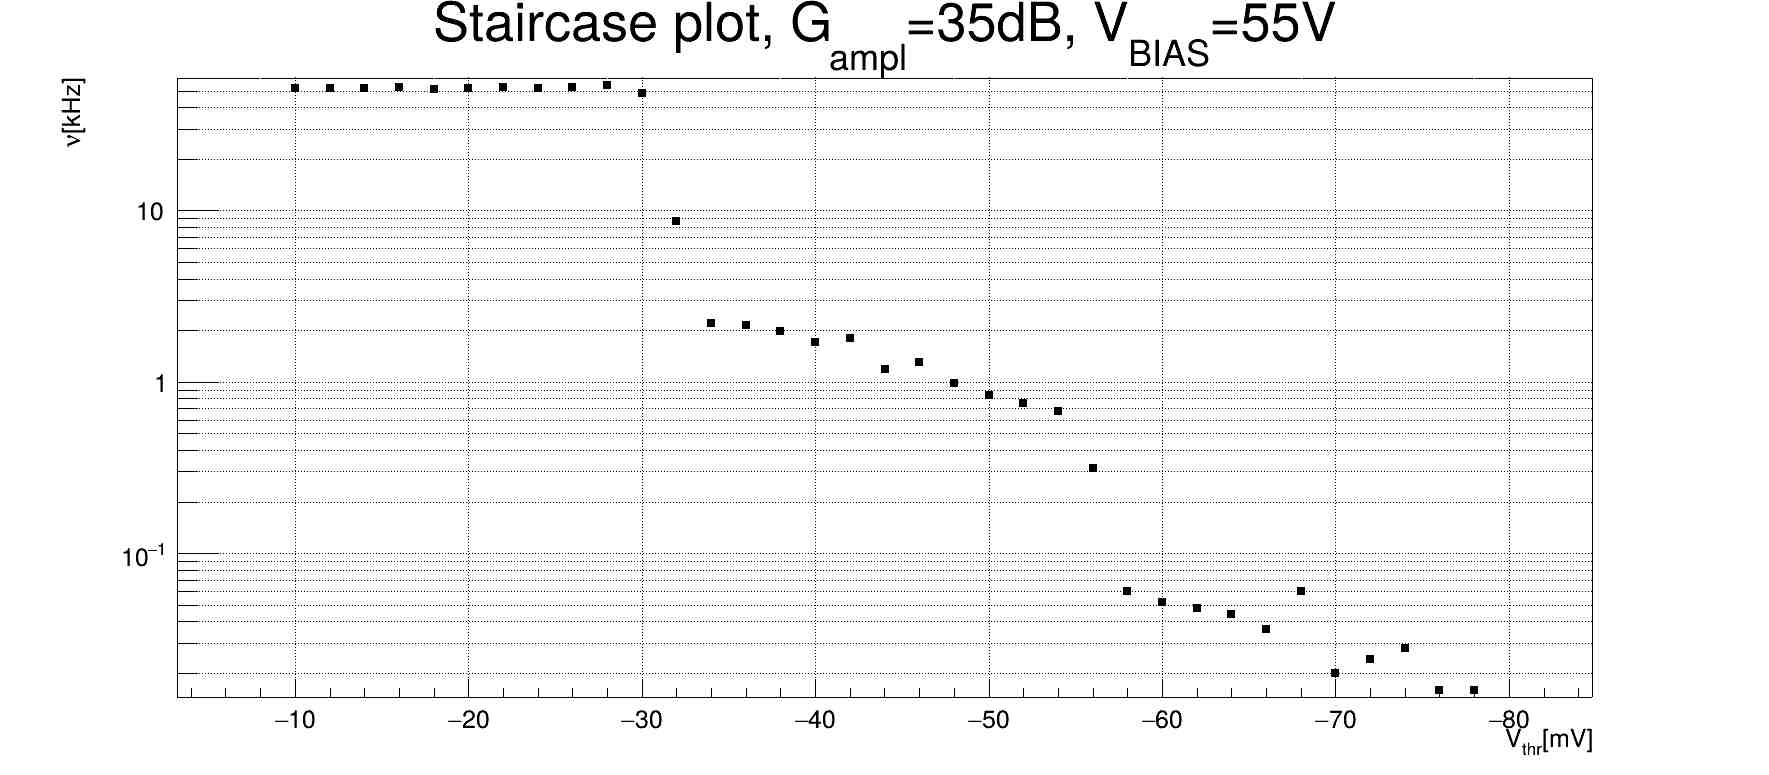
\includegraphics[width=0.82 \linewidth]{./fig1/dcr_stair.jpg}
    \caption{\footnotesize \textit{Staircase plot} a $G_{ampl}=35$dB e $V_{bias}=55$V.}
    \label{fig:DCR_stair}
\end{figure}

Dal grafico \ref{fig:DCR_stair} si osserva il caratteristico andamento a gradini: gli scalini di frequenza si collocano in corrispondenza delle tensioni $V_{out,i}$, multipli interi di $V_{out,1}$, associata a un solo pixel acceso. 

Per ottenere la miglior stima del DCR, si effettuano misure ripetute del \textit{rate} a una tensione di soglia $V_{thr} = -17$mV fissata a circa metà del primo livello e con un intervallo di tempo di acquisizione $\Delta{t}$ (\textit{gate width}) prestabilito. 
Si effettua dunque un fit gaussiano sulla distribuzione dei conteggi ottenuta, da cui vengono estratti il valore atteso $N_1$ di impulsi ricevuti nell'intervallo $\Delta{t}_1$ e la sua deviazione standard $\sigma_{N,1}$.
La miglior stima del \textit{rate}, data dal rapporto tra $N_1$ e il gate $\Delta{t}$, è 
$$\nu_1 = (51.1  \pm  0.4 ) \text{ kHz } $$
Per l'analisi dell'\textit{optical cross talk} è necessario ripetere lo stesso procedimento a fissata $V_{thr} = -44$mV (circa a metà del secondo gradino); in questo modo si ottiene la stima del \textit{rate} per il secondo livello $\nu_2$: 
$$\nu_2 = (1.23  \pm0.05 ) \text{ kHz } $$
\begin{multicols}{2}
\begin{figure}[H]
    \centering
    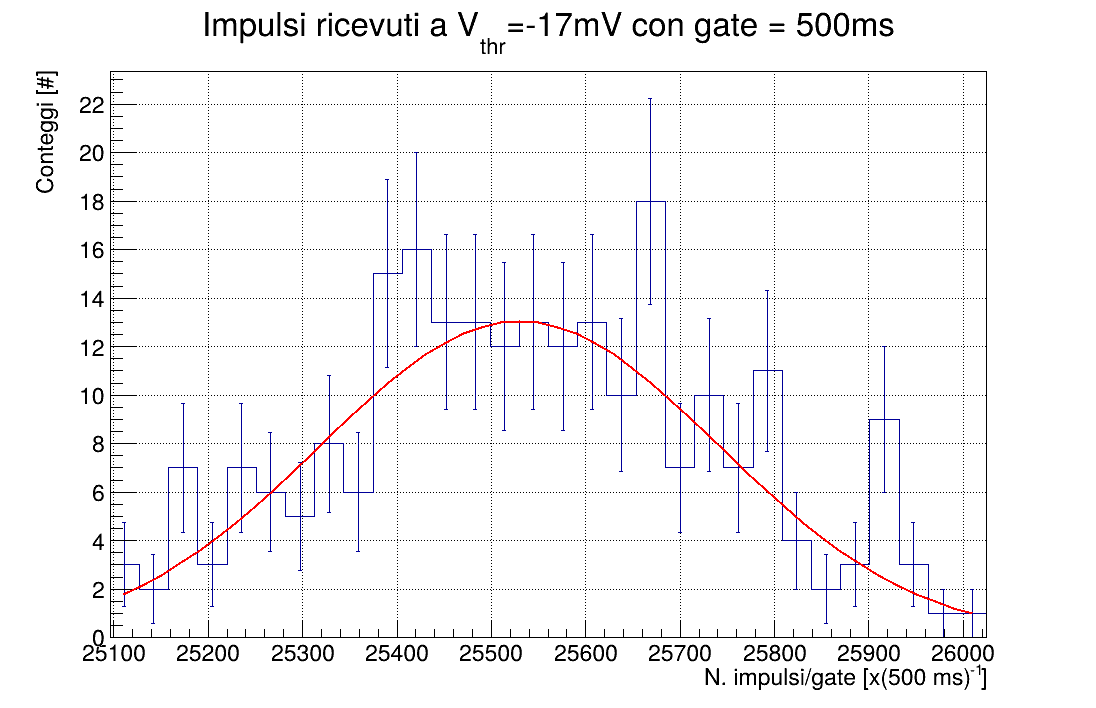
\includegraphics[width=0.99\linewidth]{./fig1/dcr_17.png}
    \caption{\footnotesize Istogramma dei conteggi per numero di impulsi ricevuti a $V_{thr}=-17$ mV e \textit{gate width} di 500 ms; in rosso è rappresentato il fit gaussiano: parametri estratti $N_1= (25530 \pm  16) $CHN e $\sigma_{N,1}= ( 211 \pm  15 ) \text{CHN}$, $\chi^2=23.7$ e 27 d.o.f.}
\end{figure}

\begin{figure}[H]
    \centering
    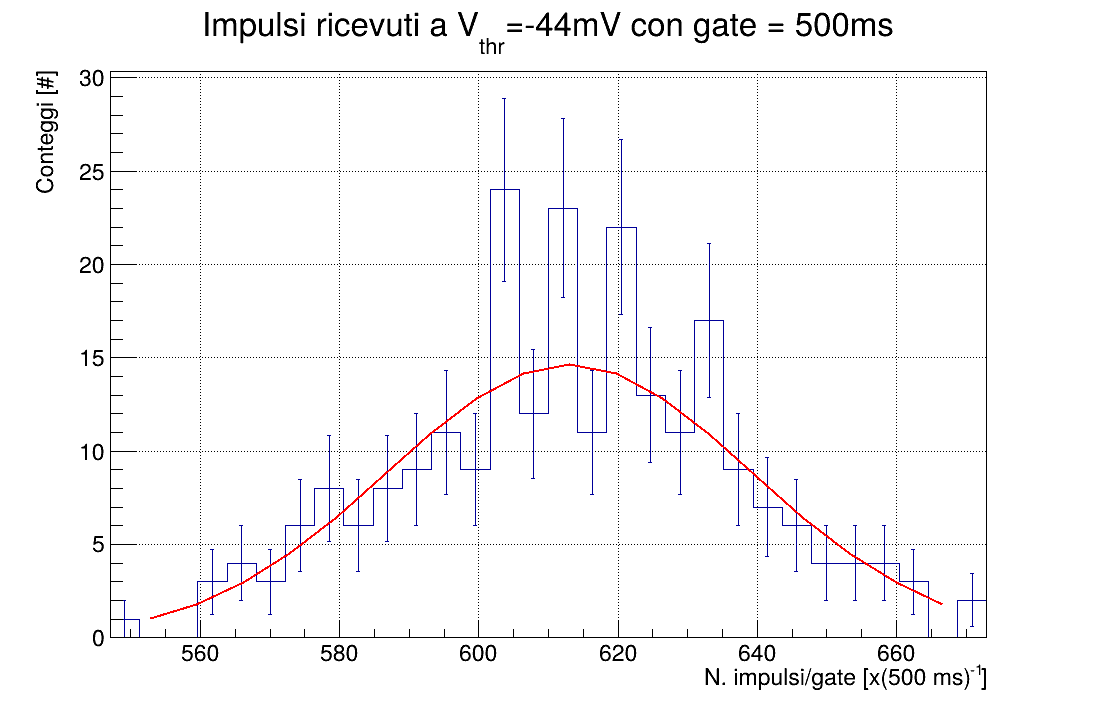
\includegraphics[width=0.99\linewidth]{./fig1/dcr_44.png}
    \caption{\footnotesize Istogramma dei conteggi per numero di impulsi ricevuti a $V_{thr}=-44$ mV e \textit{gate width} di 500 ms; in rosso è rappresentato il fit gaussiano: parametri estratti $N_2= ( 613 \pm  2) \text{ CHN }$ e $\sigma_{N,2}= ( 26 \pm  2 ) \text{ CHN }$, $\chi^2=19.0$ e 23 d.o.f.}
\end{figure}
\end{multicols}

\textit{Osservazione.} È stato possibile stimare soltanto i \textit{rate} dei primi due livelli $\nu_1$ e $\nu_2$ poichè, come evidenziato dal grafico \ref{fig:DCR_stair}, lo strumento non è sensibile alle frequenze troppo basse.




L'\textit{optical cross talk} (OCT) è definito come il rapporto tra il \textit{rate} corrispondente all’accensione di \textit{almeno due} celle $\nu_2$ e il rate misurato all’accensione di \textit{almeno una} singola cella $\nu_1$, $$OCT = \frac{\nu_2}{\nu_1}$$
ed è conseguenza del fatto che la valanga di carica prodotta da una cella può scatenarne un'altra in una cella vicina.
\\
Utilizzando le stime di $\nu_1$ e $\nu_2$ si ricava la frazione di eventi in cui è avvenuto l'\textit{optical cross talk}.
$$ OCT = (2.4  \pm0.1  ) \text{ \% } $$
Questa stima è in linea con il valore atteso per SiPM con queste caratteristiche.
\subsubsection{DCR e OCT in funzione della temperatura del sistema}
In questa sezione si analizza il comportamento del DCR e dell'OCT al variare della temperatura \textit{T} del sistema, prima del raggiungimento della condizione di stabilità termica del SiPM.\\
Subito dopo aver acceso il SiPM, sono stati raccolti sette volte i valori della temperatura e le due distribuzioni di conteggi per numero di impulsi ricevuto, una a fissata $V_{thr,1}$ per il primo gradino e l'altra a fissata $V_{thr,2}$ per il secondo gradino\footnote{La tesione di soglia $V_{thr}$ è stata sempre scelta circa a metà del gradino}. In appendice 5.1 vengono riportati gli istogrammi delle due distribuzioni e i relativi fit gaussiani per il calcolo di DCR e OCT.
\begin{table}[H]
    \centering
    \begin{tabular}{|c|c|c|c|}
        \hline
        
        \textbf{T[$^o$C]} & \textbf{$\mathbf{\nu_1}$ (DCR)[kHz]} & \textbf{$\mathbf{\nu_2}$ [kHz]} & \textbf{OCT=$\mathbf{\nu_2/\nu_1}$ [\%]} \\ \hline
        
        $20.4  \pm  0.5 $  &  $16.6  \pm  0.2  $  &  $ 0.27 \pm  0.02 $  &  $1.63  \pm  0.13 $ \\ \hline
        $22.1  \pm  0.3 $  &  $17.59  \pm  0.18  $  &  $0.29  \pm  0.5 $  &  $1.7  \pm  0.3 $ \\ \hline
        $22.7  \pm  0.2 $  &  $18.4  \pm  0.3  $  &  $0.276  \pm  0.012 $  &  $1.50  \pm  0.07 $ \\ \hline
        $23.0  \pm  0.1 $  &  $19.1  \pm  0.2  $  &  $0.29  \pm  0.02 $  &  $1.52  \pm  0.11 $ \\ \hline
        $23.4 \pm  0.1 $  &  $19.7  \pm  0.2  $  &  $0.29  \pm  0.02 $  &  $1.49  \pm  0.11 $ \\ \hline
        $23.7  \pm  0.1 $  &  $20.20  \pm  0.19  $  &  $0.30  \pm  0.03 $  &  $1.50  \pm  0.13 $ \\ \hline
        $23.9  \pm  0.1 $  &  $20.75  \pm  0.16  $  &  $0.293  \pm  0.019 $  &  $1.41  \pm  0.09 $ \\ \hline
        
    \end{tabular}
    \caption{\footnotesize Valori di temperatura del sistema $T$, \textit{rate} $\nu_1$ (DCR), \textit{rate} $\nu_2$ e OCT=$\nu_2$/$\nu_1$ alla tensione $V_{bias}=55$V e \textit{gain} $G_{ampl}=35$dB.}
    \label{tab:temp}    
\end{table}

\textit{Osservazione.} Siccome non è possibile acquisire i due istogrammi simultaneamente e la temperatura del SiPM varia velocemente, molte coppie di istogrammi sono in realtà riferite a due valori diversi di temperatura, $T_1$ e $T_2$, di cui si è calcolata la media e la semidispersione.

Separatamente vengono graficate le coppie di valori ($T_j$,$DCR_j$) e ($T_i$,$OCT_i$) e si effettua su ciascun grafico una regressione lineare sui dati, dimostrando che il DCR dipende linearmente dalla temperatura, mentre l'OCT è costante rispetto a questa.
Infatti, dall'analisi sperimentale risulta che il coefficiente angolare $a$ della retta $DCR$ in funzione di $T$, il cui valore è $a= ( 1.8 \pm  0.2 ) \text{kHz/}^o\text{C}$, risulta positivo e significativamente diverso da zero; mentre il coefficiente angolare $c$ della retta $OCT$ in funzione di $T$, il cui valore è $c= (-0.08  \pm  0.09 ) ^o\text{C}^{-1}$, risulta statisticamente compatibile con zero.
\begin{multicols}{2}
\begin{figure}[H]
    \centering
    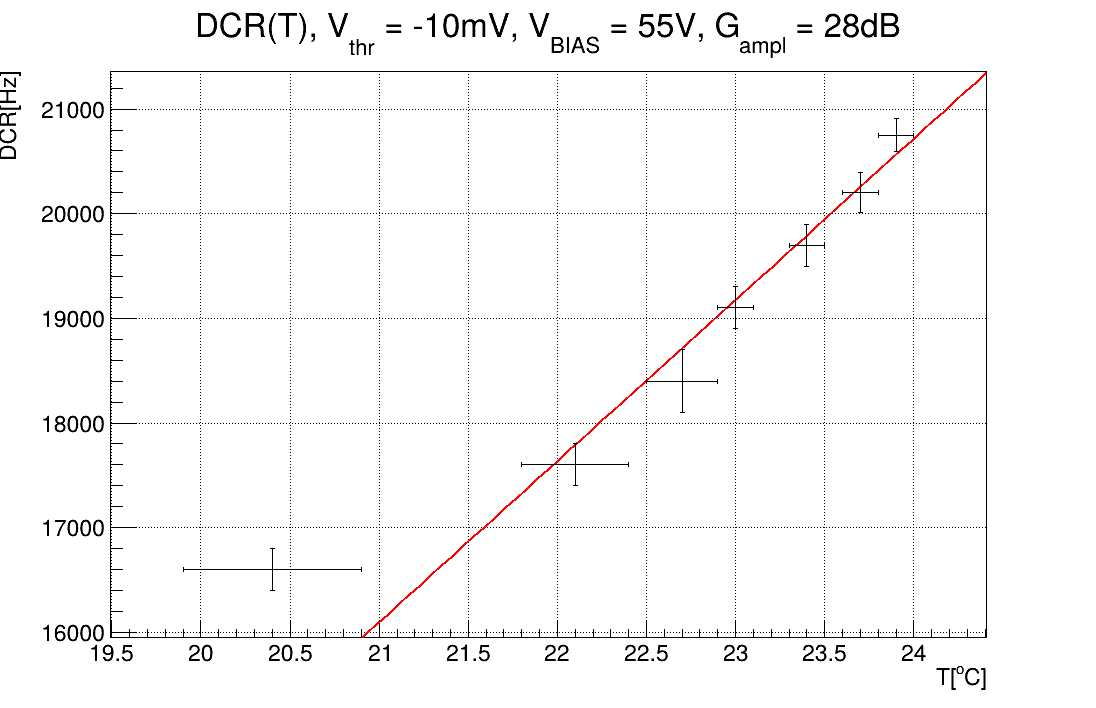
\includegraphics[width=0.99\linewidth]{fig1/DCRT.png}
    \caption{\footnotesize Grafico delle coppie ($T_j$,$DCR_j$) e fit lineare $y = ax+b$: parametri estratti $a= (1.54 \pm  0.19 ) \text{kHz/}^o\text{C}$ e $b= (-16  \pm  5 ) \text{kHz}$, $\chi^2=4.9$, d.o.f.$=5$.}
    \label{fig:DCR_T}
\end{figure}

\begin{figure}[H]
    \centering
    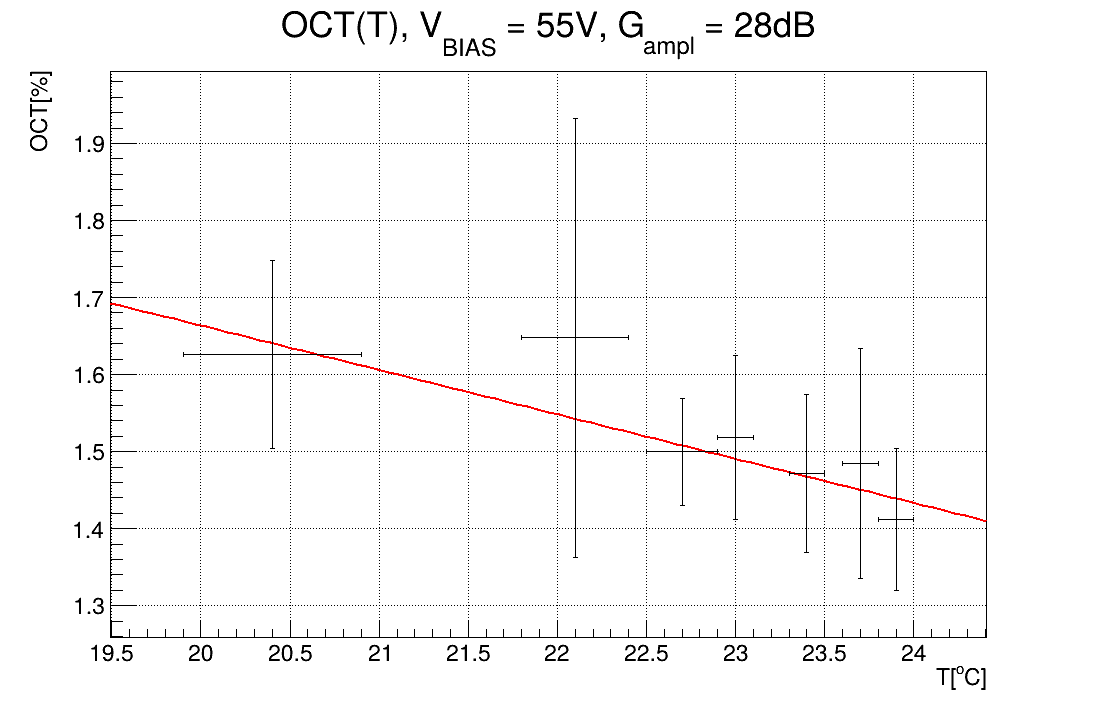
\includegraphics[width=0.99\linewidth]{fig1/OCTT.png}
    \caption{\footnotesize Grafico delle coppie ($T_i$,$OCT_i$) e fit lineare $y=cx+d$: parametri estratti $c= (-0.06  \pm  0.04 ) ^o\text{C}^{-1}$ e $d= (2.8  \pm  1.0 ) \text{\%}$, $\chi^2=0.4$, d.o.f.$=5$.}
    \label{fig:OCT_T}
\end{figure}
\end{multicols}
Per il fit dell'OCT, il valore di $\chi^2$ è molto minore del numero di gradi di libertà e questo risultato è dovuto a due fattori: in primo luogo, visto che la variazione di $T$ è avvenuta molto velocemente, le incertezze sui valori della temperatura sono abbastanza grandi; d'altra parte, anche le incertezze sui \textit{rates} risultano elevate, in quanto, per la necessità di prendere velocemente le misure, si è dovuto impostare un \textit{gate} di acquisizione abbastanza corto (500ms).

\textit{Osservazione.} Il risultato suggerisce dunque che al crescere della temperatura del sistema aumenta la probabilità che per agitazione termica si inneschi una valanga, mentre non aumenta significativamente la probabilità che la valanga di una cella accenda altre celle adiacenti.

\subsection{Caratterizzazione di un SiPM con sorgente luminosa (LED)}

Si introduce ora una sorgente luminosa (LED con $\lambda= (400 \pm 14)$nm) e si sfrutta un trigger esterno che dà inizio alla lettura ogni volta che il LED invia un impulso di luce; in questo modo non verranno conteggiati eventi dovuti al rumore intrinseco ma verranno anche conteggiate le letture nulle.

\textit{Osservazione.} Con un trigger interno, il DCR ($\nu_1 \sim 50$ kHz) avrebbe influenzato significativamente la misura, richiedendo la sottrazione dai conteggi corrispondenti all'accensione di una cella di un valore pari a $\nu_1\tau$, con $\tau\sim120$s tempo totale di acquisizione. Il trigger esterno invece permette di annullare il DCR, ma non l'OCT, il quale però è solo dell'ordine del $2\%$.

\subsubsection{Prima stima di $G_\text{SiPM}$}
Dal momento che la carica restituita da una cella attivata da un fotoelettrone viene amplificata dalla PSAU di un fattore $G_{ampl}$ espresso in unità naturali\footnote{Relazione di conversione: $G_{ampl}(dB)=20\log_{10}G_{ampl}$}, la carica totale prodotta da un singolo impulso luminoso $q_{1-cella}$ è pari a $$q_{1-cella}=G_\text{ampl}G_\text{SiPM}e$$ 
Fissati una tensione di alimentazione $V_{bias}$, un \textit{gain} di amplificazione $G_{ampl}$ e l'intensità del LED, si visualizza sul Digitizer il caratteristico spettro dei fotoelettroni riportato in figura \ref{fig:LED_Gsipm}.

\begin{figure} [H] 
    \centering
    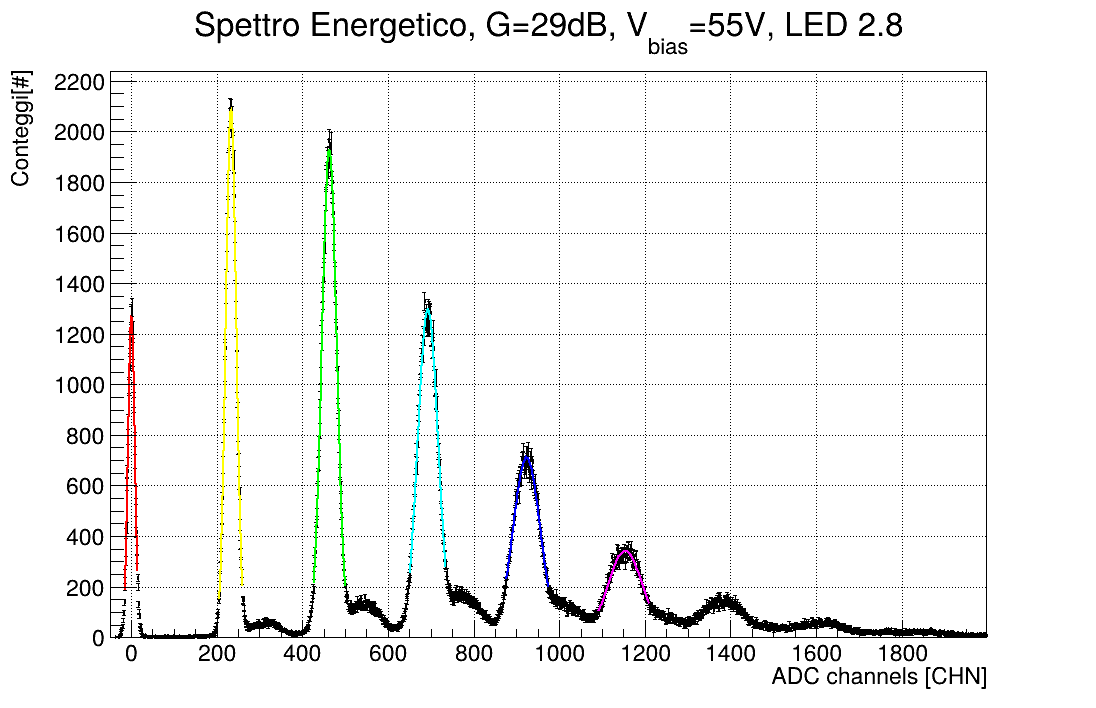
\includegraphics[width=0.60\linewidth]{fig1/led_gsipm.png}
    \caption{ \footnotesize Istogramma dei conteggi per numero di canale a $V_{BIAS}=55$V, $G_{ampl}=29$dB, intensità del LED di 2.8. e fit gaussiani ditinguibili dal colore (per ciascun fit parametri estratti, d.o.f e $\chi^2$ sono riportati nella tabella \ref{tab:gsipm} in appendice)}
    \label{fig:LED_Gsipm}
\end{figure}

\textit{Osseravzione.} Ciascun picco del grafico \ref{fig:LED_Gsipm} rappresenta un diverso numero di celle accese e la sua altezza rappresenta la quantità di volte in cui ciò avviene: in particolare, il primo rappresenta gli eventi in cui il trigger si è attivato, ma non si sono rilevati fotoni, mentre i successivi rappresentano 1, 2,... fotoni incidenti.

Inoltre, è possibile notare che i picchi sono equidistanti di $\Delta_{pp}$, corrispondente alla carica raccolta da una singola cella. Effettuando dei fit guassiani sui primi 6 picchi, da cui si estraggono i valori attesi $p_i$ e le rispettive deviazioni standard $\sigma_{p,i}$ (vedi Tabella \ref{tab:gsipm} in appendice), si possono calcolare diverse stime $\Delta_{pp, i}$ tra picchi consecutivi. Dopo aver dimostrato che queste appartengono alla stessa popolazione tramite test di Gauss, se ne fa una media pesata ottenendo $$ \langle\Delta_{pp}\rangle= (231  \pm  11 ) \text{CHN} $$
Noto il fattore di calibrazione del sistema, $k=40$ fC/CHN, la carica totale restituita da una cella $q_{1-cella}$ si può esprimere anche come $$q_{1-cella}=k\langle\Delta_{pp}\rangle$$
In conclusione, si può ottenere una prima stima del guadagno del SiPM dalla seguente formula 
\begin{equation}
    G_{SiPM}=\frac{k\Delta_{pp}}{G_{ampl}e}= (2.05  \pm  0.09 )\cdot10^6
    \label{eq:GSiPM}
\end{equation}
\textit{Osservazione.} Come ci si aspetta per il modo di funzionamento a valanga, $G_{SiPM}$ è dell'ordine di $10^6$. 

\subsubsection{Verifica della linearità dell'amplificazione della carica}
In questa sezione, si vuole dimostrare che l'intensità del segnale associata all'accensione di una singola cella $\Delta_{pp}$ cresce linearmente con l'amplificazione $G_{ampl}$; perciò a intensità del LED di 2.5 e $V_{bias}=55$V fissate, si acquisiscono gli spettri dei fotoelettroni al variare di $G_{ampl}$. \\
Da ogni spettro si ricavano le rispettive stime di $\langle\Delta_{pp}\rangle_j$ e le relative incertezze (riportate in tabella \ref{tab:gain}) seguendo lo stesso procedimento descritto nel paragrafo precedente 1.2.1. Tutti gli spettri sono riportati nell'appendice \ref{sec:app_gain}.

\begin{multicols}{2}
\begin{figure} [H]
    \centering
    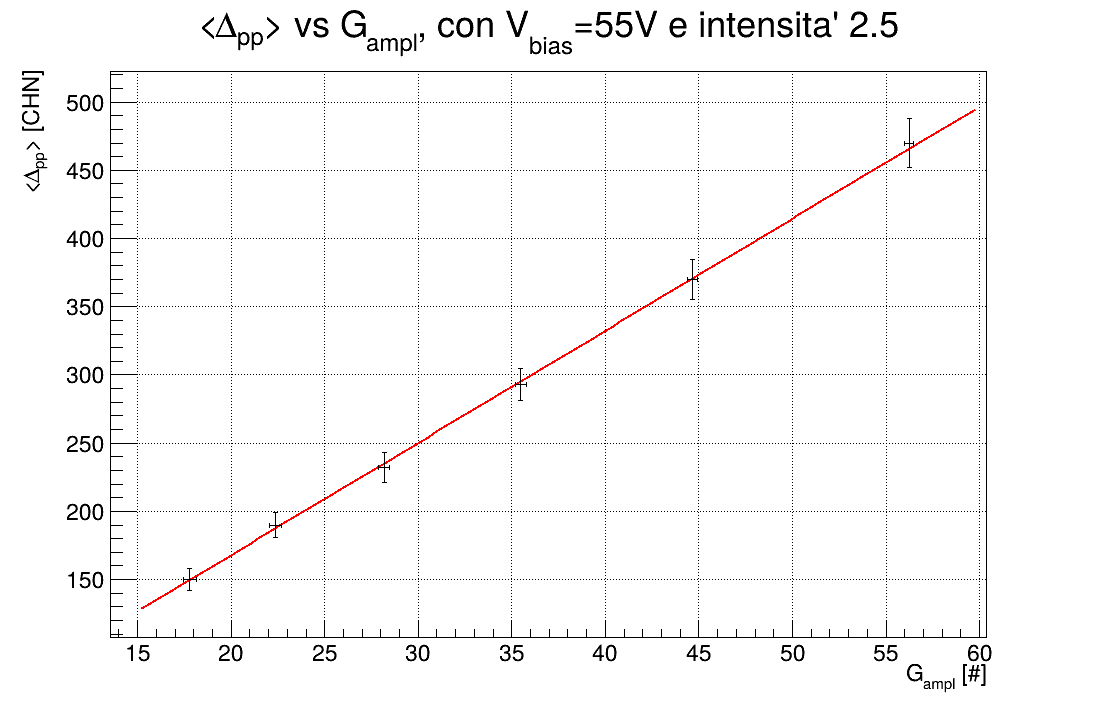
\includegraphics[width=1. \linewidth]{fig1/deltapp_G.png}
    \caption{ \footnotesize Coppie di dati ($G_{ampl,j}$,$\langle\Delta_{pp}\rangle_j$) e regressione lineare con $\chi^2=0.2$ e d.o.f.$=4$.}
    \label{fig:deltapp_G}
\end{figure}

\begin{table}[H]
    \bigskip
    \centering
     \begin{tabular}{|c|c|}
        \hline
        \textbf{$\mathbf{\langle\Delta_{pp}\rangle}$[CHN]} & \textbf{$\mathbf{G_{ampl}}$[dB]} \\ \hline
        $150 \pm 8$                                    & $25 \pm 1$                         \\ \hline
        $190 \pm 9$                                    & $27 \pm 1$                         \\ \hline
        $232 \pm 11$                                    & $29 \pm 1$                         \\ \hline
        $293 \pm 12$                                    & $31 \pm 1$                         \\ \hline
        $370 \pm 15$                                    & $33 \pm 1$                         \\ \hline
        $470 \pm 18$                                    & $35 \pm 1$                         \\ \hline
    \end{tabular}
    \caption{\footnotesize Valori di \textit{gain} di amplificazione e distanza picco-picco media $\langle\Delta_{pp}\rangle_j$ alla tensione $V_{bias}=55$V e con intensità LED 2.5.}
    \label{tab:gain}
\end{table}

\end{multicols}
Dal grafico \ref{fig:deltapp_G} delle coppie di dati ($G_{ampl,j}$,$\langle\Delta_{pp}\rangle_j$) si evince una dipendenza lineare di $\langle\Delta_{pp}\rangle_j$ con il \textit{gain} di amplificazione del tipo $\langle\Delta_{pp}\rangle_j=a \cdot G_{ampl,j}+b$. I valori estratti dal fit lineare risultano: $ a =  (8.2  \pm  0.4 ) \text{CHN} $ e $ b = (4  \pm  13)$CHN.

Il valore di $\chi^2 = 0.2$ del fit è molto piccolo rispetto al numero di gradi di libertà; questo è da attribuirsi al fatto che per stimare le posizioni dei picchi dei vari spettri energetici si sono utilizzate le deviazioni standard delle singole gaussiane $\sigma_{p,i}$ come errori sulle medie delle stesse: gli errori relativi, specialmente nei picchi a valori di CHN maggiori, risultano quindi piuttosto grandi.

Il parametro $a$ ottenuto dal fit lineare risulta compatibile tramite test di Gauss con quello che si ricava da $ a = \frac{G_\text{SiPM}\cdot e}{k} = (8.21  \pm  0.04 ) \text{ CHN }$ dalla relazione \ref{eq:GSiPM}, usando il valore di $G_{SiPM}$ stimato nella sezione precedente (equazione \ref{eq:GSiPM}). La compatibilità statistica assicura dunque che il coefficiente angolare della retta di fit ha il significato fisico atteso. \\
Allo stesso modo, il valore di $b$ ottenuto risulta statisticamente compatibile con zero.

\textit{Osservazione.} I risultati appena ottenuti, a meno di una costante moltiplicativa, hanno permesso di dimostrare che la carica totale restituita all'accensione di una singola cella,\\$q_{1-cella}=k\langle\Delta_{pp}\rangle$, aumenta linearmente con il \textit{gain} di amplificazione regolabile dalla \textit{PSAU}.

\subsubsection{$G_\text{SiPM}$ in funzione della tensione $V_\text{bias}$}
Al fine di poter studiare l'andamento del guadagno del SiPM $G_{SiPM}$ in funzione di $V_{bias}$ vengono mantenuti costanti l'intensità del LED a 2.5 e il \textit{gain} di amplificazione a $29$dB.\\
Sperimentalmente è possibile ripetere la stessa procedura vista nel paragrafo precedente per l'ottenimento delle stime di $\langle\Delta_{pp}\rangle$ da ogni spettro e dunque stimare il $G_{SiPM}$ usando la relazione \ref{eq:GSiPM} al variare della tensione $V_{bias}$. In appendice 5.2.3 sono riportati tutti gli spettri di fotoelettroni. \\
Si ottengono così cinque coppie di valori di ($G_{SiPM,k}$, $V_{bias,k}$), riportate in tabella \ref{tab:vbias}, le quali suggeriscono un andamento lineare e crescente; per verificare tale ipotesi, si è effettuata una regressione lineare sui dati, riportata in figura \ref{fig:vbias_G}.

\begin{multicols}{2}
\begin{figure} [H]
    \centering
    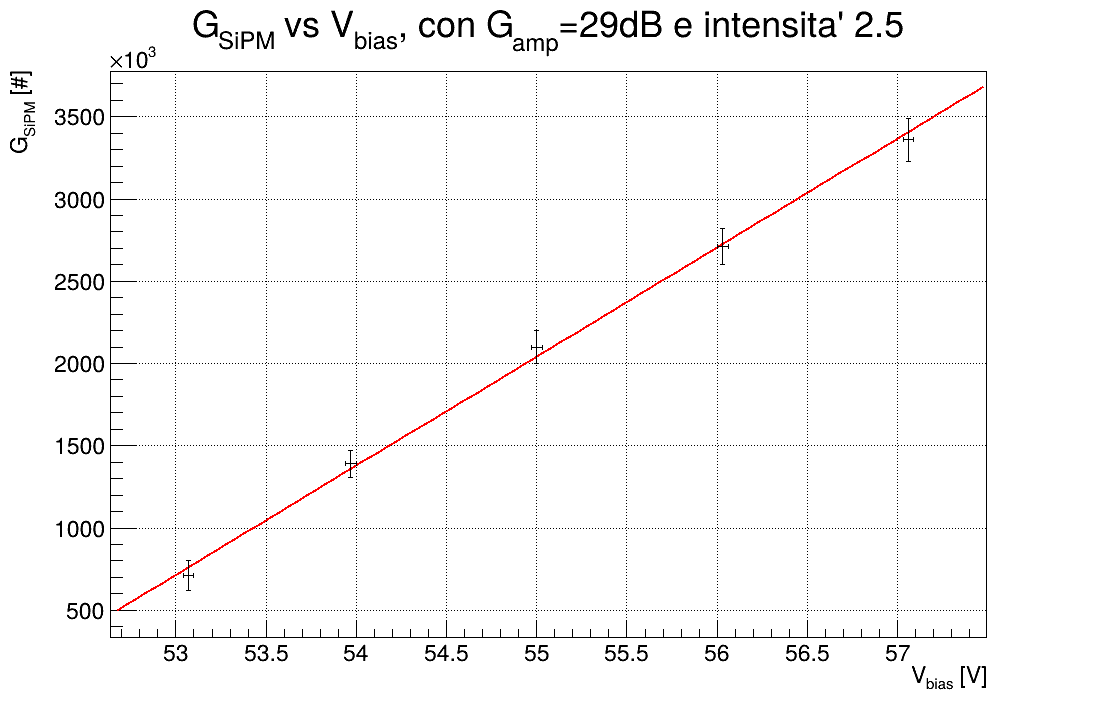
\includegraphics[width=.94\linewidth]{fig1/led_vbias.png}
    \caption{ \footnotesize Coppie di valori ($V_{bias,j}$, $G_{SiPM,j}$) e regressione $G_{SiPM}=a+b\cdot V_{bias}$ con parametri restituiti $a= ( 6.6 \pm 0.3 )\cdot10^5 \text{ V }^{-1}$, $b = (-3.45\pm0.18)\cdot10^7$, $\chi^2=0.7$ e d.o.f.$=3$}
    \label{fig:vbias_G}
\end{figure} \phantom{.}

\begin{table}[H]
\centering
    \begin{tabular}{|c|c|}
    \hline
    $\mathbf{G_\textbf{SiPM}}$\textbf{[\#]} & $\mathbf{V_\textbf{bias}}$\textbf{[V]} \\
    \hline
    $ (710 \pm 90)\cdot 10^3 $ &$ 53.07 \pm 0.03$ \\
    \hline
    $ (1.39 \pm 0.08)\cdot 10^6$ &$ 53.97 \pm 0.03$ \\
    \hline
    $ (2.1 \pm 0.1)\cdot 10^6$ &$ 55.00 \pm 0.03$ \\
    \hline
    $ (2.71 \pm 0.11)\cdot 10^6$ &$ 56.03 \pm 0.03$ \\
    \hline
    $ (3.36 \pm 0.13)\cdot 10^6$ &$ 57.06 \pm 0.03$ \\
    \hline
    \end{tabular}
    \caption{ \footnotesize Valori di guadagno del SiPM $G_{SiPM}$ e tensione di alimentazione $V_{bias}$ a intensità del LED di 2.5 e $G_{ampl}=29$dB fissati}
    \label{tab:vbias}
\end{table}
\end{multicols}
Come nel fit lineare precedente, il valore di $\chi^2 = 0.7$ risulta molto basso e una possibile causa è la grande incertezza sulle medie dei picchi degli spettri energetici.

\textit{Osservazione.} L'andamento crescente con la tensione di alimentazione è spiegabile con il fatto che aumentando la tensione di polarizzazione inversa delle celle aumenta la portata della valanga e dunque il guadagno del SiPM. \\

\subsubsection{Stima del numero di fotoni $\mu_{ph}$ rivelati in funzione dell'intensità del LED}

Si determina infine il numero medio di celle del SiPM colpite per 3 diverse intensità luminose del LED, mantenendo costanti la tensione di alimentazione $V_{bias} = 55$V e l'amplificazione della PSAU $G_{ampl} = 29$dB. 

\begin{figure} [H]
    \centering
    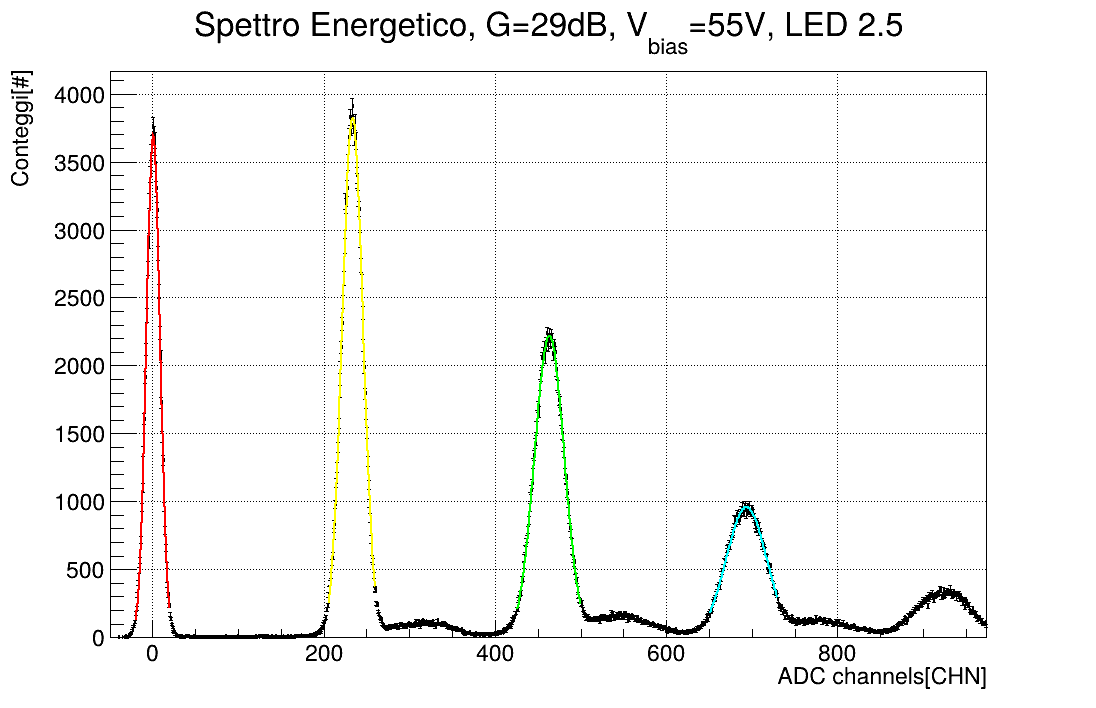
\includegraphics[width=.65\linewidth]{fig1/led_2_5.png}
    \caption{ \footnotesize Istogramma dei conteggi per numero di canale a $V_{BIAS}=55$V, $G_{ampl}=29$dB, intensità del LED di 2.5. e fit gaussiani distinguibili dal colore (per ciascun fit d.o.f e $\chi^2$ sono riportati nella tabella \ref{tab:led2_5} in appendice)}
    \label{fig:led_I_2_5}
\end{figure}

Il numero medio di fotoelettroni può essere stimato in due modi, uno più approssimativo e uno più accurato.

Il metodo approssimativo consiste nello stimare la media dell'istogramma $\langle CHN\rangle$ e la distanza media tra i picchi $\langle\Delta_{pp}\rangle$: il numero medio di fotoelettroni è stimato dal rapporto
$$\mu_{ph} = \frac{\langle CHN\rangle}{\langle\Delta_{pp}\rangle}$$
Nella tabella \ref{tab:I} di seguito sono riportate le stime di $\langle CHN\rangle$, $\langle\Delta_{pp}\rangle$ e $\mu_{ph}$ al variare dell'intensità del LED.

\begin{table}[H]
\centering
    \begin{tabular}{|c|c|c|c|}
    \hline
    $\mathbf{I_{LED}}$ & $\mathbf{\langle \Delta_{pp}\rangle}$ \textbf{[CHN]} & $\mathbf{\langle CHN \rangle} $\textbf{[CHN]} &$ \mathbf{\mu_{ph}}$ \\
	\hline
    $2.0$ &$ 232.60\pm0.04 $ &$191.1\pm0.3$ &$0.8216\pm0.0014$ \\
    \hline
    $2.5$ &$231.71\pm0.04$ &$379.4\pm0.4$ &$1.6375\pm0.0018$ \\
    \hline
    $2.8$ &$231.02\pm0.05$ &$675.0\pm0.6$ &$2.922\pm0.003$ \\
    \hline
    \end{tabular}
    \caption{\footnotesize Valori di $\langle CHN\rangle$, $\langle\Delta_{pp}\rangle$ e $\mu_{ph}$ al variare di $I_{LED}$; gli spettri per $I_{LED} = 2.0$ e $I_{LED} = 2.8$ si possono trovare in appendice 5.2.4}
    \label{tab:I}
\end{table}
Il metodo accurato consiste invece nel calcolare l'area $A_N$ sottesa a ciascun fit gaussiano, che corrisponde al numero di volte in cui si sono accese $N$ celle contemporaneamente, e associarla tramite un istogramma al numero di picco $N$; dato il basso numero punti a disposizione, l'andamento di questo istogramma è poissoniano e da un fit su di esso si estrae la stima di $\mu_{ph}$.

Per i tre spettri acquisiti al variare di $I_{LED}$, queste regressioni non vanno a buon fine a causa del limitato numero di gradi di libertà (causato dal ridotto numero di picchi) e della sottostima delle incertezze sulle aree degli integrali, in quanto esse derivano dalle incertezze sui parametri dei fit.

Per ciascun valore di $I_{LED}$ si verifica inoltre la relazione, prevista dalla teoria, tra le varianze dei picchi gaussiani
$$ \sigma^2_{N} = \sigma^2_{0} + N\sigma^2_{p} $$
in cui $\sigma_0^2$ è la varianza del picco corrispondente a 0 fotoelettroni, N è il numero di picco e $\sigma^2_p$ è una costante.
\begin{multicols}{2}
    \begin{figure} [H]
    \centering
    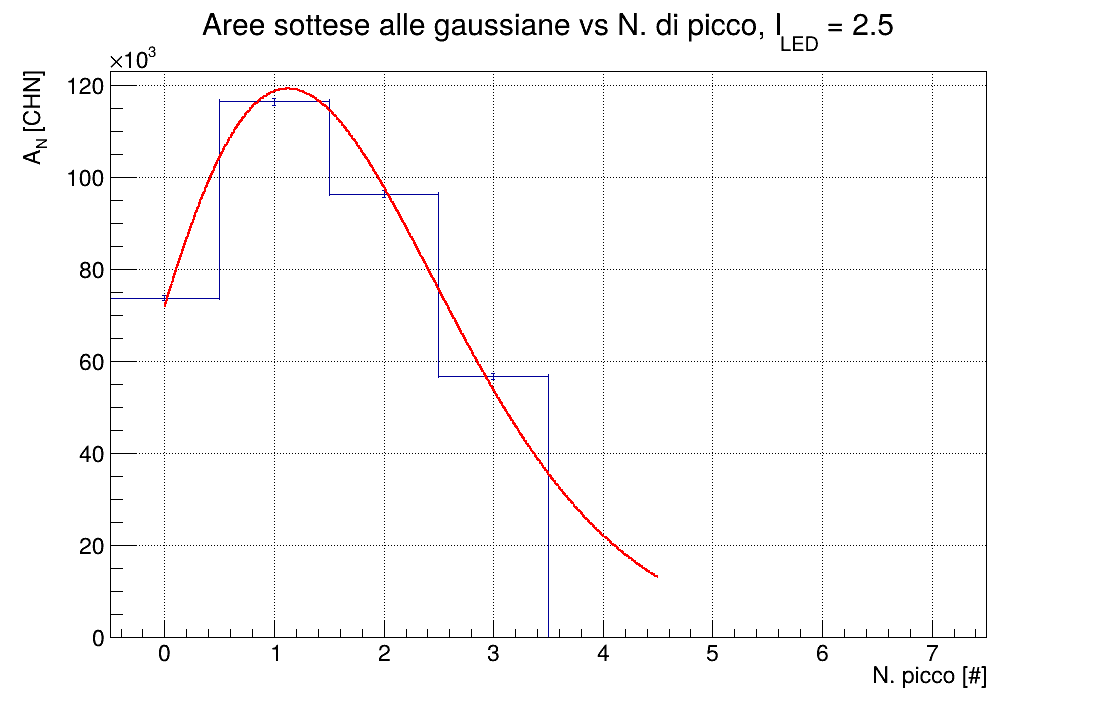
\includegraphics[width=1.\linewidth]{fig1/led_area_2_5.png}
    \caption{ \footnotesize Istogramma delle aree sottese alle gaussiane per lo spettro a $I_{LED} = 2.5$ in funzione del numero di picco con fit Poissoniano non convergente, $\chi^2 = 42$ e d.o.f$=2$.}
    \label{fig:led_pois_2_5}
\end{figure}
\begin{figure} [H]
    \centering
    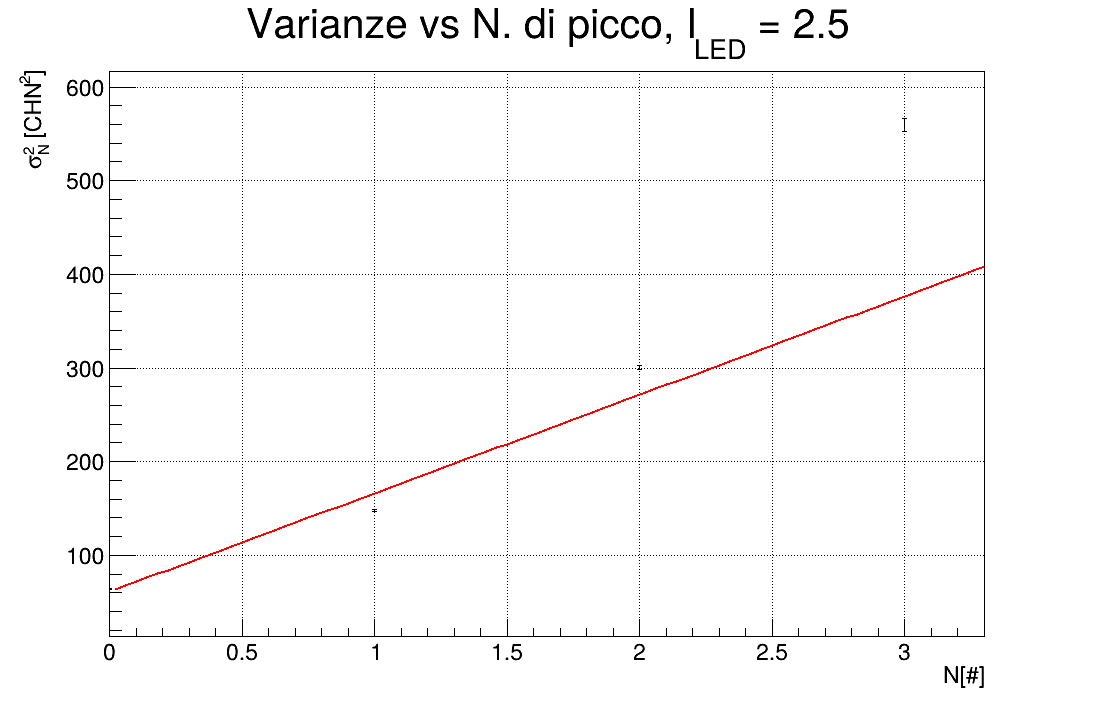
\includegraphics[width=1.\linewidth]{fig1/led_var_2_5.png}
    \caption{ \footnotesize Grafico delle varianze delle gaussiane per lo spettro a $I_{LED} = 2.5$ in funzione del numero di picco con fit lineare non convergente, $\chi^2 = 1453$ e d.o.f$=2$.}
    \label{fig:led_var_2_5}
\end{figure}
\end{multicols}
Il fit lineare non va a buon fine in nessuno dei tre casi, probabilmente per una sottostima delle incertezze sulle varianze, stimate dalle incertezze sui parametri $\sigma_N$ delle gaussiane.

I grafici dello spettro eneregetico, dell'istogramma delle aree e del grafico delle varianze per gli altri due valori di $I_{LED}$ si trovano in appendice 5.2.4.
\newpage
{\color{gray}\hrule}
\begin{center}
\section{Rivelazione della radiazione $\beta^{-}$}
\bigskip
\end{center}
{\color{gray}\hrule}    
Per la seconda parte dell'esperienza, volta alla rivelazione della radiazione $\beta^{-}$, si utilizza un Supporto SP5608 con lastra di scintillatore in polistirene (area attiva: 4.7x4.7x1 cm$^3$) avvolta in nastro di teflon e un SiPM a 14400 celle in 6.0x6.0mm$^2$; l'utilizzo di un SiPM con più celle rispetto a quello della prima parte permette di avere misure più precise, a discapito di un aumento del DCR e di una maggiore probabilità di OCT.
Inoltre, come prima, l’unità di alimentazione e amplificazione (PSAU) fornisce segnali analogici in tensione, ricevuti e convertiti in canali dal Digitizer.

La radiazione di tipo $\beta^{-}$ ha origine dal decadimento di un neutrone $n$ in un protone $p$ con l'emissione di un elettrone $e^-$ e un anti-neutrino elettronico $\bar \nu_e$, $$n \rightarrow p + e^- + \bar \nu_e$$
L’elettrone emesso ($\beta^-$) può incidere sullo scintillatore, interagire con gli elettroni legati agli atomi del materiale plastico e cedere tutta la sua energia cinetica iniziale. L'energia trasferita eccita gli atomi a livelli superiori, i quali, diseccitandosi, ritornano allo stato fondamentale emettendo fotoni nel visibile (tipicamente $\lambda \approx 425$ nm). Solo una parte ($\sim30\%$) della luce di scintillazione viene rivelata dal SiPM e convertita in un segnale elettrico proporzionale al flusso di fotoni. \\ Una volta calibrato in energia lo spettro, sarà possibile caratterizzare la radiazione $\beta^-$ emessa dalle sorgenti di $^{90}\mathrm{Sr}$ e $^{137}\mathrm{Cs}$. \\
Infine, verrà analizzata la capacità di assorbimento della radiazione $\beta^-$ di due diversi materiali, alluminio e carta, con lo scopo di ricavare alcune caratteristiche di questi ultimi. \\

\subsection{Spettro ${}^{90}$Sr}
Il decadimento di ${}^{90}$Sr produce Ittrio-90 e avviene tramite emissione $\beta^-$ durante la reazione
$$^{90}\mathrm{Sr} \rightarrow {}^{90}\mathrm{Y} + e^- + \bar{\nu}_e $$
A sua volta, anche $^{90}\mathrm{Y}$ decade in Zirconio-90 tramite emissione $\beta^-$, seguendo $$^{90}\mathrm{Y} \rightarrow {}^{90}\mathrm{Zr} + e^- + \bar{\nu}_e $$
\textit{Osservazione.} Si anticipa che il tempo di dimezzamento dell'Ittrio-90 è tanto piccolo rispetto a quello dello Stronzio-90 da non permettere di isolare i due spettri, che risulteranno quindi sovrapposti.
\subsubsection{Fattore di calibrazione $k_{Sr}$ dell'apparato con sorgente in asse}
Una volta posizionata la sorgente in asse con il fotomoltiplicatore, si acquisisce dal Digitizer uno spettro costituito da circa 2 milioni di eventi. Durante l’intera fase di presa dati è fondamentale mantenere il sistema quanto più possibile isolato dalla luce esterna, così da minimizzare il rumore; inoltre, si utilizza come \textit{trigger} esterno il segnale proveniente dallo stesso SiPM, impostando una soglia di discriminazione $V_{thr}$\footnote{Per tutta questa sezione si è impostato $V_{thr} = -6$ mV} in corrispondenza del punto in cui termina l'andamento esponenziale del \textit{rate} visualizzabile sullo Staircase plot.

\textit{Osservazione.} Il rivelatore SiPM+scintillatore è adatto per spettroscopia $\beta^-$ in quanto le particelle provenienti dalla sorgente si fermano nel polistirene cedendo tutta la loro energia cinetica iniziale. Lo spettro in energia che si ottiene è approssimabile all'energia degli elettroni acquisita nella reazione di decadimento. Quest'ultima inoltre non è monocromatica ma varia in modo continuo da 0 ad un valore massimo $T_{max}$. 

Si riporta di seguito lo spettro in energia di ${}^{90}$Sr con sorgente in asse.
\begin{figure} [H]
    \centering
    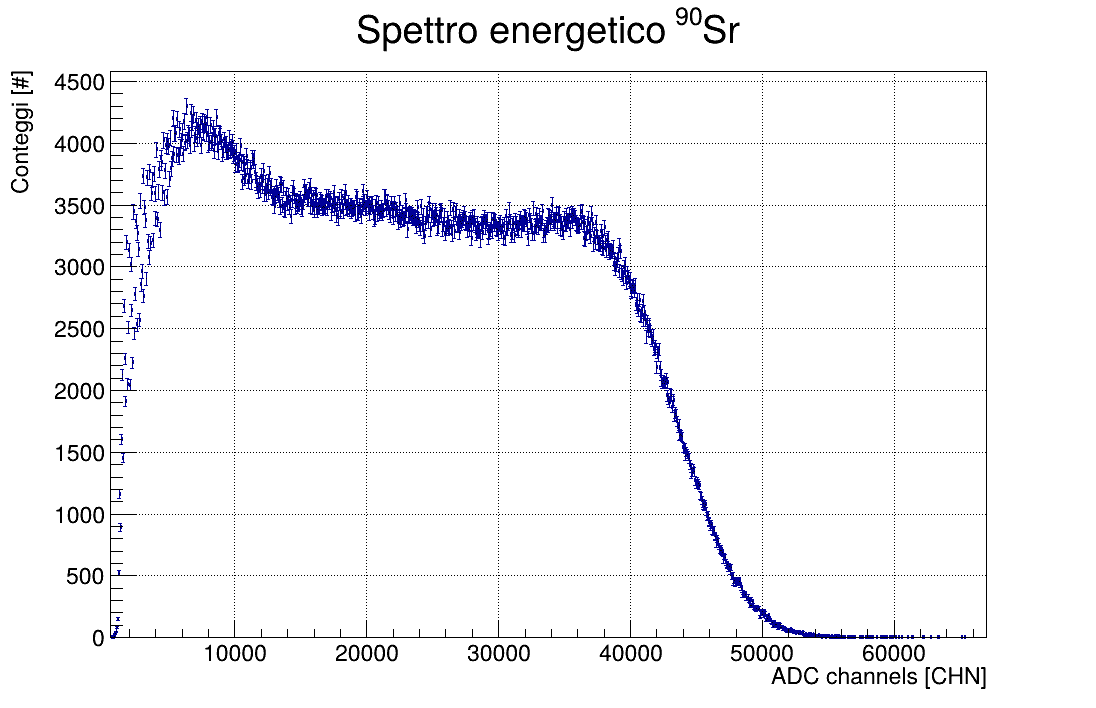
\includegraphics[width=0.65\linewidth]{fig2/sr90_tot.png}
    \caption{ \footnotesize Istogramma di conteggi per numero di canale dello ${}^{90}$Sr}
    \label{fig:Sr90_tot}
\end{figure}

L'istogramma mostra la sovrapposizione dei due spettri: in particolare si osserva un contributo a energie più basse associato a ${}^{90}\mathrm{Sr}$, mentre ${}^{90}\mathrm{Y}$, 
caratterizzato da un’\textit{end-point} $T_{0,Y}$ maggiore, domina la regione a energie più elevate, determinando l’estensione complessiva dello spettro.\\
La sovrapposizione degli spettri impedisce di riconoscere il $T_{0,Sr}$ dello Stronzio-90, mentre è possibile misurarne il $T_{max, Sr}$; viceversa, per l'Ittrio-90 non è individuabile il $T_{max, Y}$, mentre è possibile misurarne il $T_{0, Y}$.

Dalla misura sperimentale dell'\textit{end-point} $CHN_{0,Y}$ dell'Ittrio-90 è possibile ricavare la costante di calibrazione $k_{Sr}$ del sistema mediante la formula 
\begin{equation}
    k_{Sr}=\frac{T_{0,Y}}{CHN_{0,Y}}
    \label{eq:k}
\end{equation} dove in letteratura l'\textit{endpoint} dello Ittrio-90 è $T_{0,Y}= (2.28\pm 0.04)$ MeV.\\
Per ottenere una stima di $CHN_{0,Y}$, nella regione di \textit{end-point} si effettua un plot di Kurie, consistente in una regressione lineare sulle coppie di dati ($\frac{\sqrt{conteggi}}{CHN}$,$CHN$), riportata di seguito nel grafico \ref{fig:kurie_cen}.

\begin{figure} [H]
    \centering
    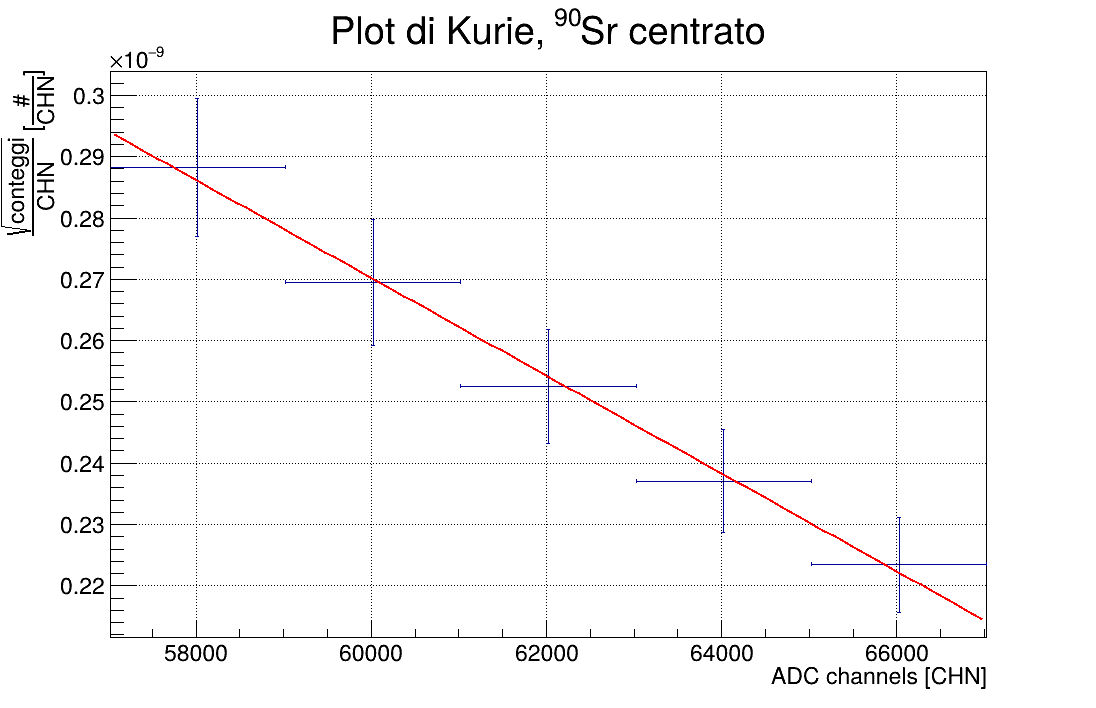
\includegraphics[width=0.65\linewidth]{fig2/kurie_cen.png}
    \caption{ \footnotesize Istogramma ($CHN$,$\frac{\sqrt{conteggi}}{CHN}$) e regressione lineare $y=a+bx$ con parametri restituiti $a = ( 7.5 \pm 0.9 )\cdot 10^{-10} \text{ CHN }^{-1}$, $b= (-8.0\pm1.5)\cdot 10^{-15} \text{CHN}^{-2}$, $\chi^2=0.11$ e d.o.f.$=3$}
    \label{fig:kurie_cen}
\end{figure}

Dal fit si estrapola $CHN_{0,Y}= ( 9 \pm 2 )\cdot10^4 \text{ CHN}$

Infine, si calcola il fattore di calibrazione $k_{Sr}$ dell'apparato con sorgente in asse dalla \ref{eq:k}:
\begin{equation}
    k_{Sr}=( 2.4 \pm 0.5 )\cdot10^{-5} \text{ MeV/CHN }
    \label{eq:k_Sr}
\end{equation}
Con questa stima è possibile convertire in energia ogni valore espresso in CHN: $E=k\cdot CHN$.
\subsubsection{Verifica sperimentale di $T_{max,Sr}$}
In questa sezione, si verifica sperimentalmente che la stima del valore di energia più probabile $T_{max, Sr}$, ottenuta tramite un fit parabolico (vedi figura \ref{fig:sr90_max}) nella regione corrispondente al picco, è compatibile con il valore atteso per lo spettro dello Stronzio-90, $T_{max,Sr, att} \approx 0.38\cdot T_{0,Sr}$, dove in letteratura $T_{0,Sr}=0.546$ MeV.
\begin{figure} [H]
    \centering
    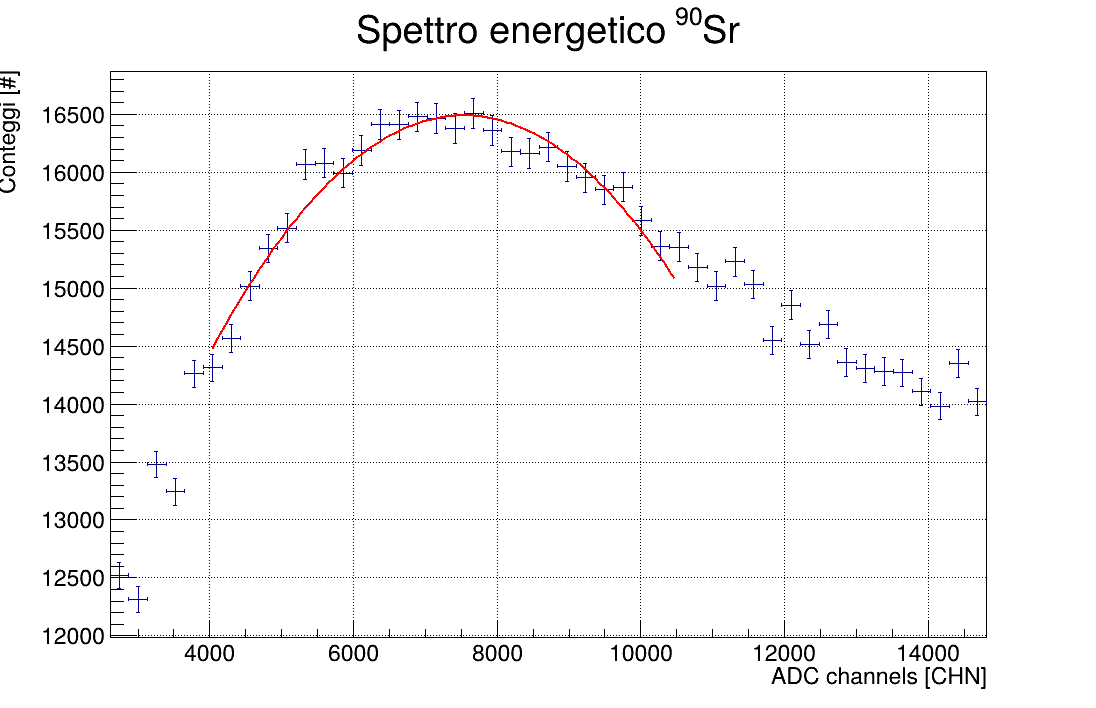
\includegraphics[width=0.64\linewidth]{fig2/sr90_max.png}
    \caption{ \footnotesize Istogramma di conteggi per numero di canali del ${}^{90}$Sr (con accorpamento di \textit{bin}) e fit parabolico $y=ax^2+bx+c$ con parametri restituiti
    $a= ( -1.64 \pm 0.08 )\cdot10^{-4} \text{ CHN }^{-2}$,
    $b= ( 2.47 \pm 0.11 ) \text{ CHN }^{-1}$,
    $c= 7200 \pm 400 $,
    , $\chi^2=30$ e d.o.f.$=22$}
    \label{fig:sr90_max}
\end{figure}
Prima si è estratta dal fit parabolico la stima del picco $CHN_{max, Sr}=( 7.5 \pm 0.5 )\cdot10^3 \text{ CHN }$ che è stata poi convertita in energia: $$T_{max, Sr}= ( 0.18 \pm 0.04 ) \text{ MeV }$$
che è statisticamente compatibile con il valore atteso.

\subsubsection{Fattore di calibrazione $k_{Sr,eq}$ dell'apparato con sorgente fuori asse}
Si ripete l’acquisizione dello spettro di ${}^{90}$Sr posizionando la sorgente in una configurazione fuori asse, ovvero a una distanza $r_{eq}$ dal centro dello scintillatore. \\Si può dimostrare infatti che il fattore di calibrazione medio $k_\text{Sr,eq}$, nel caso in cui i segnali colpiscano con uguale probabilità qualsiasi punto della lastra, è equivalente a quello ottenuto per una sorgente puntiforme posta a una distanza $r_{eq} = 0.3826 \cdot l$ dal centro, dove $l$ rappresenta il lato dello 
scintillatore quadrato. \\
Tale scelta consente quindi di stimare il nuovo fattore di calibrazione $k_{Sr,eq}$, utile successivamente per le misure dei raggi cosmici, poiché gli eventi non provengono da una sorgente puntiforme, ma da tutte le direzioni.\\
Dunque, analogamente a quanto fatto nel paragrafo 2.2.1, si procede all’analisi dei dati con il plot di Kurie (vedi grafico \ref{fig:kurie_decen}). 
\begin{figure} [H]
    \centering
    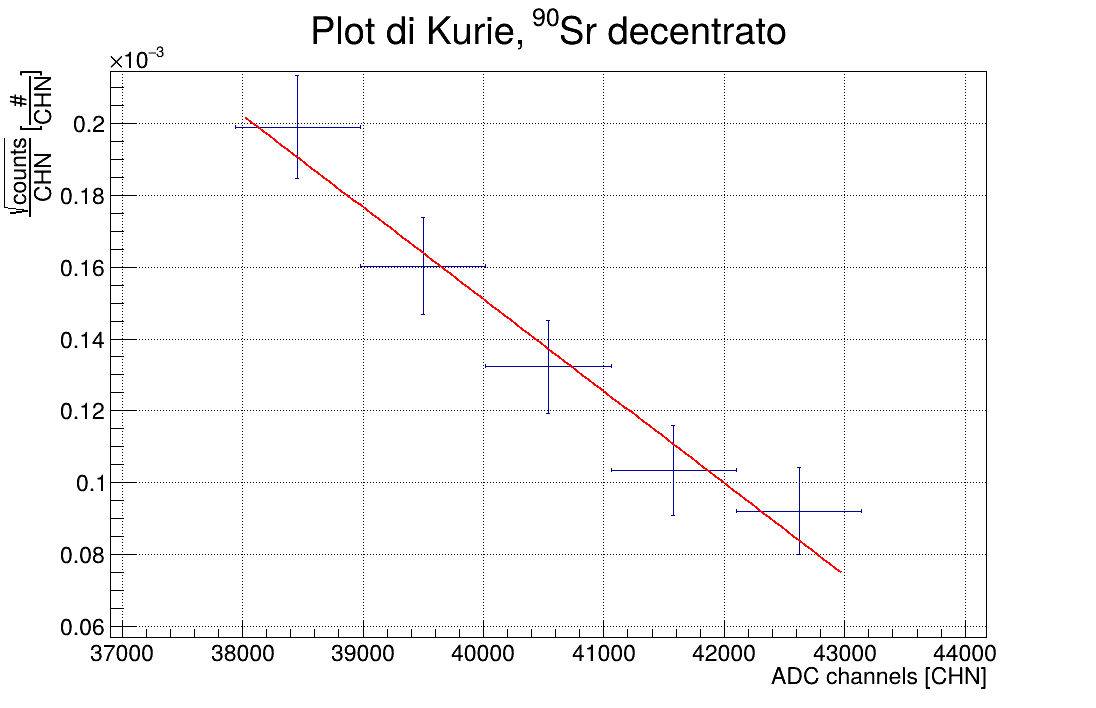
\includegraphics[width=0.7\linewidth]{fig2/kurie_decen.png}
    \caption{ \footnotesize Istogramma ($CHN$,$\frac{\sqrt{conteggi}}{CHN}$) e regressione lineare $y=a+bx$ con parametri restituiti $a= ( 1.18 \pm 0.16 )\cdot10^{-3}\text{ CHN }^{-1}$, $b= ( -2.6 \pm 0.4 )\cdot10^{-8} \text{ CHN }^{-2}$, $\chi^2=1.4$ e d.o.f.$=3$}
    \label{fig:kurie_decen}
\end{figure}

Come prima, dal fit si estrapola $CHN_{0,Y}= ( 4.6 \pm 1.0 )\cdot10^4 \text{ CHN}$ e si ricava infine il nuovo fattore di calibrazione $k_{Sr,eq}$ dell'apparato con sorgente fuori asse dalla formula \ref{eq:k}:
$$k_{Sr,eq}=( 5.0 \pm 1.0 )\cdot10^{-5} \text{ MeV/CHN }$$
Con $k_{Sr,eq}$ è possibile convertire in energia i valori espressi in CHN: $E=k_{Sr,eq}\cdot CHN$. \\

\subsection{Assorbimento della radiazione $\beta^{-}$ nei materiali} 
Tra la sorgente ${}^{90}$Sr e il rivelatore si inseriscono in modo crescente da 1 a 20 foglietti di carta o alluminio e, a gruppi di 2 o 3, se ne misurano i corrispondenti \textit{rate}, effettuando anche anche una misura senza foglietti.

Segue l'analisi per entrambi i materiali.

\subsubsection{Assorbimento con carta}
Tramite un calibro (sensibilità $0.05$mm) si misura lo spessore di un foglietto di carta $d_{carta}$ a partire dallo spessore totale dei 20 foglietti. $$d_{carta} = ( 0.100 \pm 0.003 ) \text{ mm} $$ 
Per ogni istogramma dei conteggi per numero di impulsi ricevuti associato all'aggiunta dei foglietti, si estraggono\footnote{Come per il \textit{dark count rate}, si è impostato un \textit{gate} di 500ms e si è riconvertita la stima in Hz.} media $\nu_i$ e deviazione standard $\sigma_{\nu,i}$, riportati in tabella \ref{tab:carta}. Tutti gli istogrammi sono riportati in appendice 5.3.1.

Si grafica il \textit{rate} $\nu $ in funzione dello spessore e si effettua sui dati un fit esponenziale per verificare legge di assorbimento dei raggi $\beta^-$: 
\begin{equation}
    N(x) = N(0)e^{-\mu x}
    \label{eq:assorb}
\end{equation}
dove N è il numero di particelle trasmesse dal materiale, $x$ spessore del materiale e $\mu$ coefficiente di assorbimento.\\
\begin{multicols}{2}
    \begin{figure} [H]
    \centering
    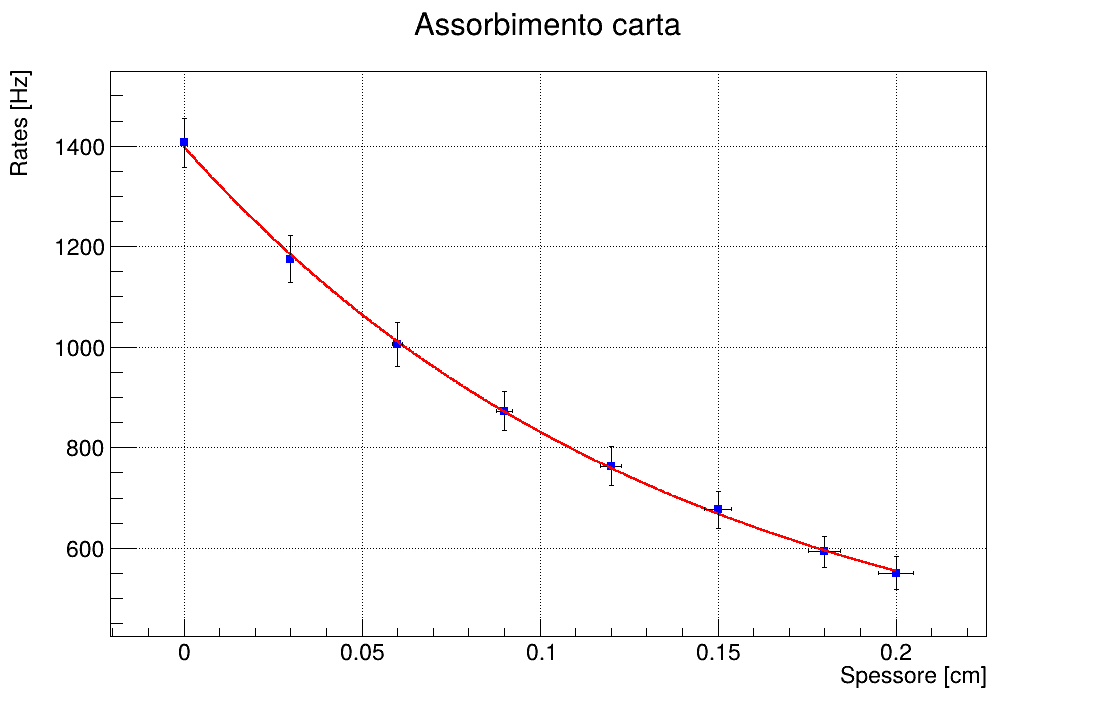
\includegraphics[width= \linewidth]{fig2/ass_carta.png}
    \caption{ \footnotesize Coppie di dati ($x$,$\nu$) e fit esponenziale \\ $y=a+be^{-cx}$ con parametri restituiti $a= ( 2.9 \pm 1.5 ) \text{$10^{2}$ Hz}$, $b= ( 11.1 \pm 1.3 ) \text{ $10^{2}$ Hz}$, $c= ( 7 \pm 2 ) \text{cm$^{-1}$ }$ e $\chi^2=0.15$ e d.o.f.=$5$}
    %\label{fig:2.3}
\end{figure}
\begin{table}[H]
    \centering
    \begin{tabular}{|c|c|c|c|}
        \hline
        
        \textbf{$n$[$\#$]} & \textbf{$x$[mm]} & \textbf{$(\nu \pm \sigma_\nu )$[$10^{2}$ Hz]} \\ \hline
        
        $ 0$  &  $ 0.000  \pm  0.003 $  &  $ 14.1 \pm  0.5 $   \\ \hline
        $ 3 $  &  $ 0.300  \pm  0.008 $  &  $ 11.8  \pm  0.5 $   \\ \hline
        $ 6 $  &  $ 0.600  \pm  0.015 $  &  $ 10.1  \pm  0.4 $  \\ \hline
        $ 9 $  &  $ 0.90  \pm  0.02 $  &  $ 8.7  \pm  0.4 $   \\ \hline
        $ 12 $  &  $ 1.20  \pm  0.03 $  &  $ 7.6  \pm  0.4 $  \\ \hline
        $ 15 $  &  $ 1.50  \pm  0.04 $  &  $ 6.8  \pm  0.4 $   \\ \hline
        $ 18 $  &  $ 1.80  \pm  0.05 $  &  $ 6.0  \pm  0.3 $  \\ \hline
        $ 20 $  &  $ 2.00  \pm  0.05 $  &  $ 5.5  \pm  0.3 $   \\ \hline
        
    \end{tabular}
    \caption{\footnotesize Valori di numero di foglietti $n$, spessore di materiale attraversato $x$, media $\nu$ e rispettiva deviazione std $\sigma_{\nu}$ alla tensione $V_{bias}=54$V e \textit{gain} $G_{ampl}=28$dB.}
    \label{tab:carta}    
\end{table}

\end{multicols}

Il parametro $c$ estratto dal fit fornisce una stima del coefficiente di assorbimento $$\mu_{carta} = ( 7\pm 2 ) \text{ cm$^{-1}$}$$ Il valore ottenuto è comparabile quello atteso atteso per elettroni con \textit{end point} di 2.2MeV nella carta:
$\mu_{carta,att}\in [ 3.5,6.5]\text{cm}^{-1}$. 

\textit{Osservazione.} Dalla visualizzazione dello spettro energetico di ${}^{90}$Sr con un numero crescente di foglietti di carta si osserva che la parte dello spettro più affetta dall'assorbimento del materiale è quella in corrispondenza di basse energie; le particelle incidenti con energia minore vengono infatti assorbite prima di raggiungere il rivelatore.

\subsubsection{Assorbimento con alluminio}
Al contrario, per l'alluminio si può calcolare lo spessore di un singolo foglietto $d_{Al}$ conoscendo il suo coefficiente di assorbimento $\mu_{Al}=(14.5 \pm 0.5) \text{cm}^{-1}$. \\
Per ogni istogramma dei conteggi per numero di impulsi ricevuti associato all'aggiunta dei foglietti, si estraggono\footnote{Come per la carta, si è impostato un \textit{gate} di 500ms e si è riconvertita la stima in Hz.} media $\nu_i$ e deviazione standard $\sigma_{\nu,i}$, riportati in tabella \ref{tab:all}. Tutti gli istogrammi sono riportati in appendice 5.3.2.\\
Si grafica il rate in funzione del numero di foglietti e si effettua sui dati un fit esponenziale per verificare legge \ref{eq:assorb} di assorbimento dei raggi $\beta^-$.\\

\begin{multicols}{2}
\begin{figure} [H]
    \centering
    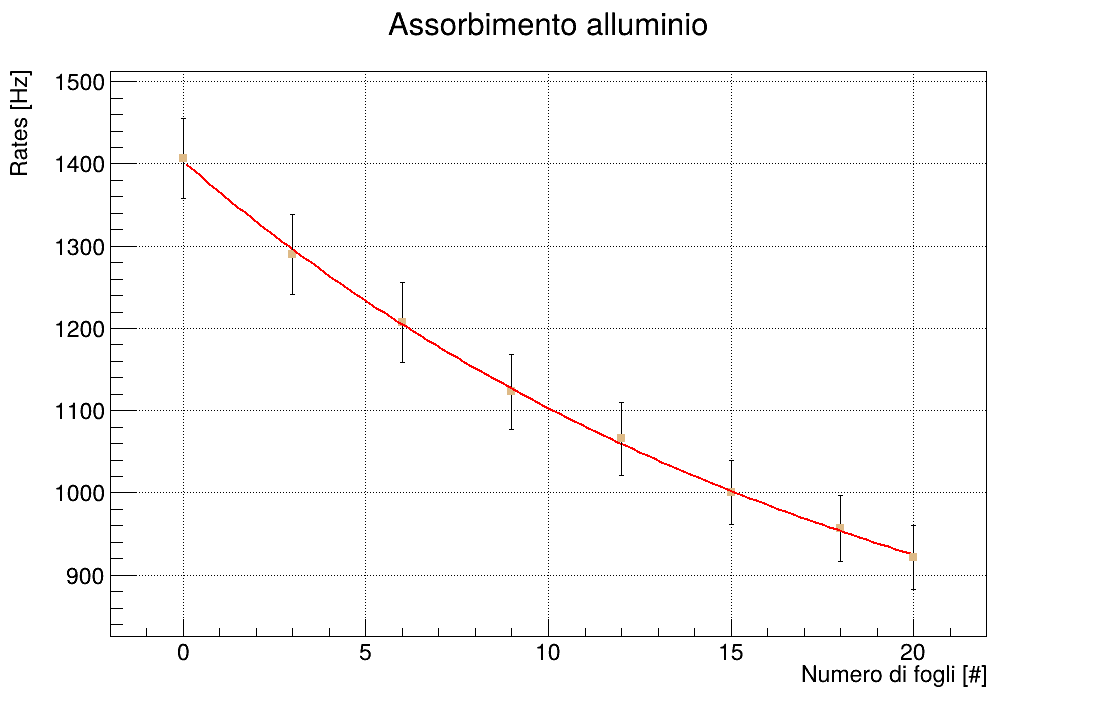
\includegraphics[width=1.\linewidth]{fig2/ass_all.png}
    \caption{ \footnotesize Coppie di dati ($n$,$\nu$) e fit esponenziale \\ $\nu=a+be^{-cn}$ con parametri restituiti $a= ( 0.7\pm 0.3 ) \text{kHz}$, $b= ( 0.7 \pm 0.3 ) \text{ kHz}$, $c= ( 0.05 \pm 0.04 ) \text{}$ e $\chi^2=0.07$ e d.o.f.=$5$}
   % \label{fig:2.3}
\end{figure}

\begin{table}[H]
    \centering
    \begin{tabular}{|c|c|c|}
        \hline
        
        \textbf{$n$[$\#$]} & \textbf{$(\nu \pm \sigma_\nu )$[$10^{2}$Hz]}  \\ \hline
        $ 0 $  &  $ 14.1  \pm  0.5 $  \\ \hline        
        $ 3 $  &  $ 12.9  \pm  0.5 $  \\ \hline
        $ 6 $  &  $ 12.1  \pm  0.5 $   \\ \hline
        $ 9 $  &  $ 11.2  \pm  0.5 $  \\ \hline
        $ 12 $  &  $ 11.0  \pm  0.4 $   \\ \hline
        $ 15 $  &  $ 10.0  \pm  0.4 $  \\ \hline
        $ 18 $  &  $ 9.6  \pm  0.4 $ \\ \hline
        $ 20 $  &  $ 9.2  \pm  0.4 $  \\ \hline
        
    \end{tabular}
    \caption{\footnotesize Valori di numero di foglietti $n$, media $\nu$ e deviazione std $\sigma_{\nu}$ alla tensione $V_{bias}=54$V e \textit{gain} $G_{ampl}=28$dB.}
    \label{tab:all}    
\end{table}
\end{multicols}

Questa volta, dal fit si estrae il prodotto $c=\mu_{Al}d_{Al}$, allora la stima dello spessore di un singolo foglietto di alluminio usando il valore teorico di $\mu_{Al}$ è $$d_{Al}= ( 0.04 \pm 0.03 ) \text{ mm}$$

Come per la carta, all'aumentare del numero di foglietti di alluminio la parte di spettro che subisce un maggior assorbimento è quella in corrispondenza delle basse energie.
\newpage
\subsection{Spettro ${}^{137}\text{Cs}$}
Nel $94.6\%$ dei casi il decadimento del Cesio-137 in Bario-137 avviene tramite emissione $\beta^-$ seguendo la reazione $$^{137}\mathrm{Cs} \rightarrow {}^{137}\mathrm{Ba(^*)} + e^- + \bar{\nu}_e $$
dove $^{137}\mathrm{Ba(^*)}$ è una forma instabile del Bario-137, la quale a sua volta può diseccitarsi emettendo un $\gamma$ con una probabilità dell'85.1$\%$:
$$^{137}\mathrm{Ba(^*)} \rightarrow {}^{137}\mathrm{Ba} + \gamma$$
Poiché la sorgente non è infinitamene sottile, la radiazione $\gamma$ emessa può estrarre per effetto fotoelettrico radiazione $\beta^-$ monocromatica:
\begin{equation}
    E_e = E_{\gamma} - B_e
    \label{eq:gamma}
\end{equation}
Tale fenomeno prende il nome di conversione interna; inoltre il $\beta^-$ estratto da $\gamma$ può appartenere a due K-shell diverse, rispettivamente a più bassa e a più alta energia di legame (624 keV e \\ 656 keV).

In alternativa, il Cesio-137 può decadere nel $5.4\%$ dei casi già nel livello stabile del Bario-137 
$$^{137}\mathrm{Cs} \rightarrow {}^{137}\mathrm{Ba} + e^- + \bar{\nu}_e $$


\subsubsection{Misura del picco di conversione interna $E_{ci}$}
Si acquisisce lo spettro completo in energia del ${}^{137}$Cs, riportato nella figura \ref{fig:cesio}, per la misura del picco di conversione interna $E_{ci}$.

\begin{figure} [H]
    \centering
    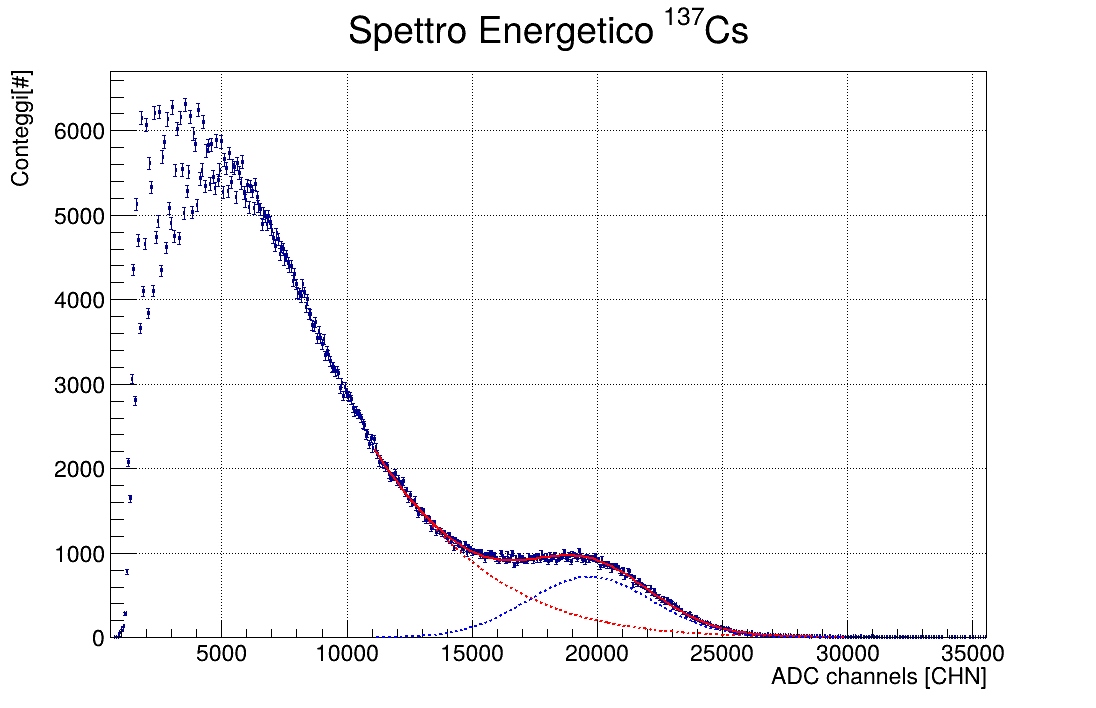
\includegraphics[width=0.75\linewidth]{fig2/cs137_conv_int.png}
    \caption{ \footnotesize Istogramma di conteggi per numero di canale del ${}^{137}$Cs, con fit di due gaussiane sovrapposte, $\chi^2=325$ e d.o.f$=286$. Sono state rappresentate le due gaussiane sommate con linee tratteggiate.}
    \label{fig:cesio}
\end{figure}

Dal grafico si può osservare l'effetto della conversione interna in corrispondenza del  secondo picco. Questo è in realtà generato dalla sovrapposizione dei due picchi relativi alle due K-shell diverse, ma la capacità risolutiva dello strumento non permette di distinguerli.

Si effettua allora un fit combinato della coda destra di una gaussiana per modellare l'andamento decrescente e di una gaussiana nella zona del picco di conversione interna. I parametri con le relative incertezze del fit sono riportate in appendice 5.2.4.

Si estraggono dal fit la posizione del picco dal valore medio della gaussiana $\langle CHN\rangle_{ci}$ e la sua deviazione standard $\sigma_{\langle CHN\rangle}$
$$\langle CHN\rangle_{ci} = ( 20 \pm 3 )\cdot10^3 \text{ CHN }$$ Convertendo in energia tramite la stima del fattore di calibrazione dello Stronzio-90 $k_{Sr}$ (\ref{eq:k_Sr}) si ottiene il valore sperimentale del picco di conversione interna $$\langle E\rangle_{ci} = ( 470 \pm 120 ) \text{ keV }$$
È stata infine verificata la compatibilità statistica tra la stima sperimentale $\langle E\rangle_{ci}$ e il valore teorico $E_{ci,att}$, ottenuto dalla media pesata\footnote{Con peso 4 per il picco teorico a $624$keV e peso 1 per quello a $656$keV} tra le energie dei due picchi:
$$E_{ci,att} = ( 629 \pm 16 ) \text{ keV }$$
Da questi parametri si stima anche la risoluzione sperimentale
\begin{equation}
R_\text{exp} = \frac{\sigma_{\langle CHN\rangle}}{\langle CHN_{ci}\rangle} = 0.128\pm0.016
\label{eq:R_exp}
\end{equation} 
\subsubsection{Verifica sperimentale di $T_{max,Cs}$}
In questa sezione viene eseguito un fit parabolico (vedi figura \ref{fig:cs_tmax}) nella regione di spettro del ${}^{137}$Cs intorno al primo picco per poter stimare il valore più probabile della distribuzione, $T_{max,Cs}$.
Dal fit si estrae una prima stima espressa in canali
$$CHN_{max,Cs}= ( 4300 \pm 200 ) \text{ CHN }$$
la quale convertita in energia risulta essere $$T_{max,Cs}= ( 100 \pm 20 ) \text{ keV }$$
\begin{figure} [H]
    \centering
    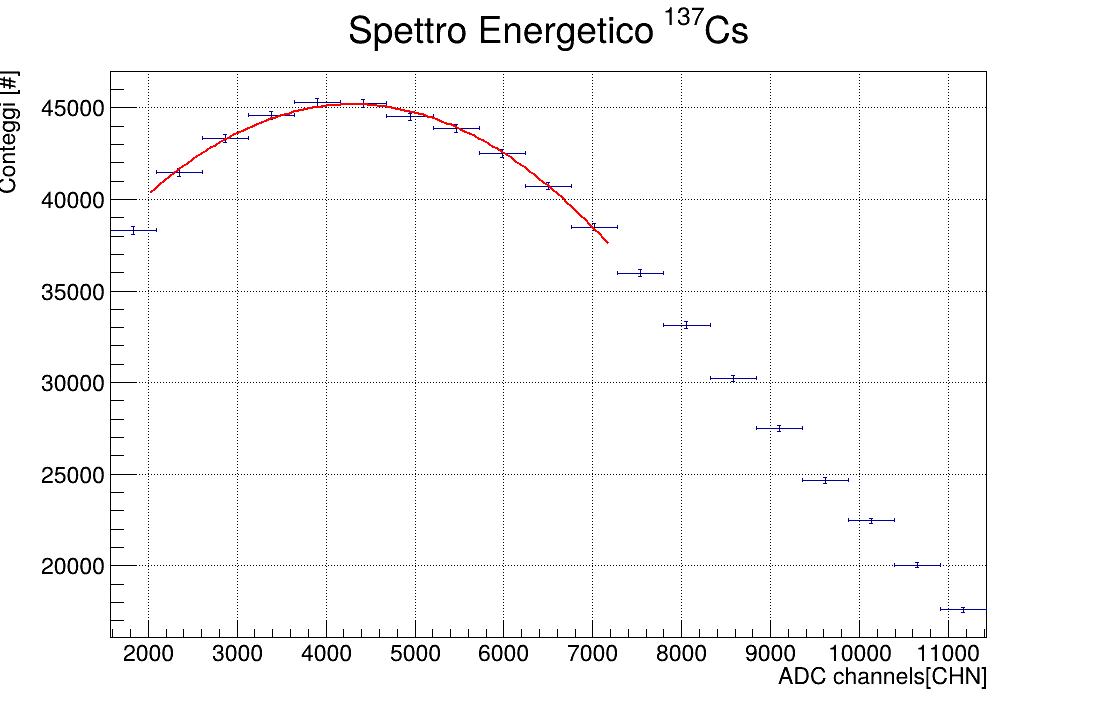
\includegraphics[width=0.65\linewidth]{fig2/cs137_Tmax.png}
    \caption{ \footnotesize Istogramma di conteggi per numero di canale del ${}^{137}$Cs (con accorpamento di \textit{bin}), con fit parabolico $y=ax^2+bx+c$ con parametri restituiti
    $a=(-9.2\pm0.3)$CHN$^{-2}$,
    $b=(7.9\pm0.3)\text{CHN}^{-1}$,
    $c=(2.81\pm0.07)\cdot10^5$, $\chi^2 = 5.8$ e d.o.f.$=7$.
    }
    \label{fig:cs_tmax}
\end{figure}
\newpage
Questa stima \textit{non} risulta statisticamente compatibile con il valore atteso (Z-score$=2.26$)
$$T_\text{max,Cs,att} = (153.6\pm0.3)\text{keV}$$
Questo è probabilmente dovuto in primo luogo al fatto che l'incertezza associata al massimo deriva da quelle sui parametri dei fit (e risulta quindi sottostimata), in secondo luogo al fatto che intorno al massimo, come si vedrà nella sezione successiva, l'andamento dell'istogramma è la sovrapposizione di diversi massimi locali che è stato necessario accorpare per poter determinare un solo massimo globale: questo ha probablimente influito nel peggiorare la stima di $T_\text{max,Cs}$

\subsubsection{Verifica della risoluzione attesa $\mathbf{R_{att}}$}
Si vuole ora stimare la risoluzione sperimentale dell'apparato; a tal fine si è acquisito uno spettro con zoom a bassi canali. 

\begin{figure} [H]
    \centering
    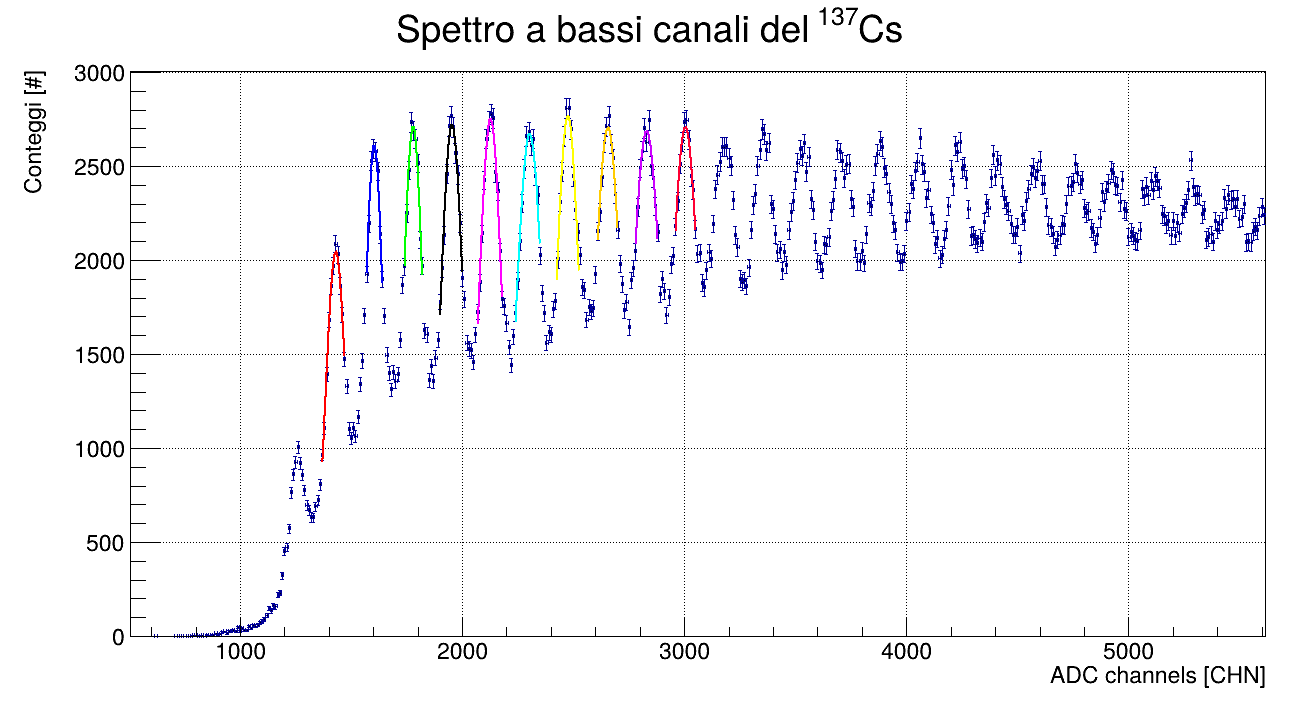
\includegraphics[width=0.82\linewidth]{fig2/fit_picchi.png}
    \caption{ \footnotesize Istogramma di conteggi per numero di canale per il ${}^{137}$Cs con zoom a bassi canali ($G_{ampl}=28$dB, $V_{bias}=54$V).}
    \label{fig:cesio-zoom1}
\end{figure}

Dal grafico \ref{fig:cesio-zoom1} si osservano i singoli picchi delle celle del SiPM accese, per ciascuno dei quali è stato effettuato un fit gaussiano da cui si sono estratti i valori medi $p_i$ e le rispettive deviazioni standard $\sigma_{p,i}$. Si possono allora calcolare diverse stime $\Delta_{pp, i}$ (vedi Tabella \ref{tab:zoomcs}) tra picchi consecutivi e dopo aver dimostrato che queste appartengono alla stessa popolazione tramite il test di Gauss, si calcolano la media pesata $\langle\Delta_{pp}\rangle$ e la sua incertezza $\sigma_{pp}$, ottenendo $$ \langle\Delta_{pp}\rangle= ( 1.7  \pm  0.3  )\cdot10^{2}\text{ CHN} $$

Si è verificato infine che la risoluzione attesa dalle caratteristiche dello strumento $$R_{att}=\sqrt{ \frac{\langle\Delta_{pp}\rangle}{\langle CHN\rangle_{ci}} \cdot \left( 1 + \left(\frac{\sigma_{pp}}{\langle\Delta_{pp}\rangle} \right)^2 \right)} =  0.095 \pm  0.009  $$ 
è statisticamente compatibile con quella sperimentale $R_{exp}$ (\ref{eq:R_exp}).









\newpage
{\color{gray}\hrule}
\begin{center}
\section{Rivelazione dei muoni cosmici }
\bigskip
\end{center}
{\color{gray}\hrule}
Dei raggi cosmici che raggiungono la superficie terrestre, i muoni $\mu^{\pm}$ rappresentano la quasi totalità, poichè hanno vita
media relativamente lunga ed essendo molto pesanti ($\approx $ 200 $m_e$) vengono poco frenati dalle interazioni in atmosfera.\\ Lo stesso kit SiPM descritto nel capitolo 2 può essere utilizzato anche per la rivelazione dei muoni cosmici, ma a differenza delle particelle $\beta^-$, per le quali è possibile effettuare spettroscopia completa, nel caso dei muoni si può parlare unicamente di frazione di energia depositata nel rivelatore, poiché essi non vengono completamente arrestati all’interno del materiale.
Lo scintillatore risulta quindi adatto anche alla rivelazione di particelle altamente energetiche (dell’ordine dei GeV), per le quali non si intende misurare l’energia totale, ma semplicemente rilevarne il passaggio.

Per ottenere uno spettro dell’energia depositata dai muoni, il rivelatore 
SiPM+scintillatore viene posizionato tra due scintillatori plastici, ciascuno 
accoppiato a un fotomoltiplicatore tramite fibra ottica.
La luce di scintillazione prodotta dal passaggio delle particelle ionizzanti 
viene così raccolta dai rispettivi fotomoltiplicatori e, nel caso di coincidenza temporale 
tra i due segnali, utilizzata come trigger esterno per il Digitizer.

\textit{Osservazione.} In questo caso non si utilizza come trigger esterno l’uscita DOUT della PSAU perché questa genera un segnale ogni volta che un impulso supera la soglia, includendo quindi anche segnali non associati al passaggio di un muone. Inoltre, a differenza del caso di una sorgente LED affrontata nel primo capitolo, il flusso
di muoni cosmici è molto basso e il loro rate è confrontabile con il \textit{dark count rate} del SiPM. Per questo motivo si sfrutta il segnale di coincidenza della \textit{Cosmic Box}, in quanto la probabilità che il rumore interno produca segnali coincidenti in entrambi i rivelatori è estremamente bassa.

\subsection{Spettro di energia depositata dai $\mu^\pm$}
Di seguito si riporta lo spettro dell'energia depositata dalle particelle acquisito in laboratorio.\\

\begin{figure} [H]
    \centering
    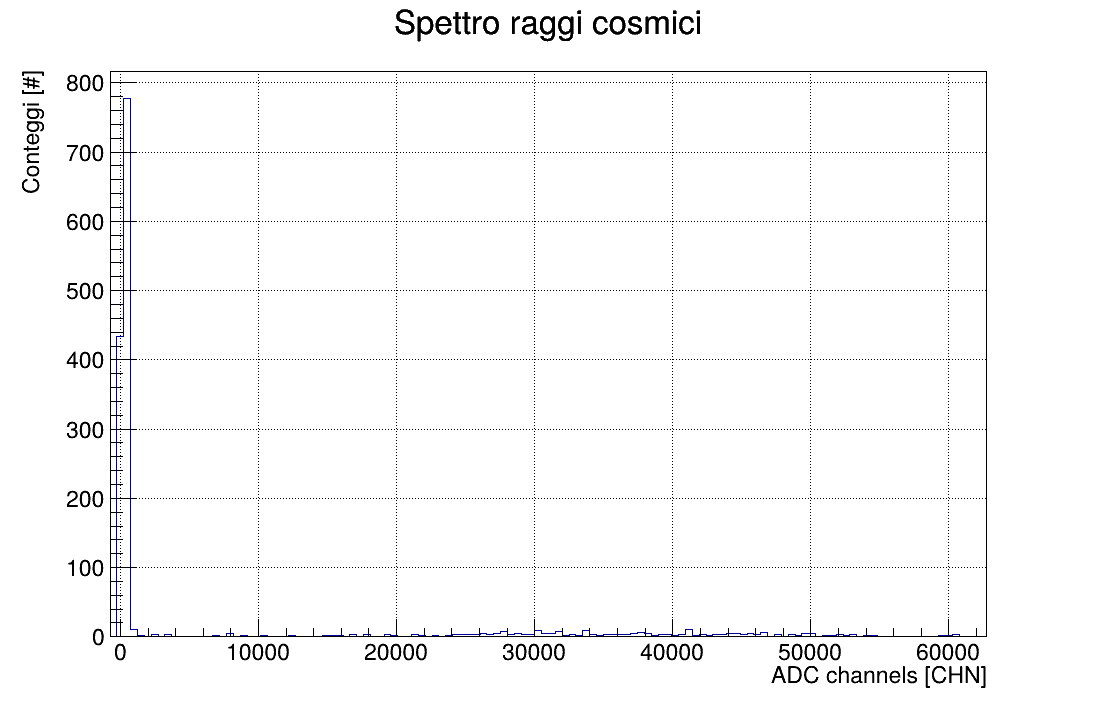
\includegraphics[width=0.62\linewidth]{fig2/raggi.png}
    \caption{ \footnotesize Istogramma di conteggi per numero di canale per i muoni cosmici completo ($G_{ampl}=28$dB e $V_{bias}=54V$).}
    \label{fig:raggi}
\end{figure}

Nel grafico \ref{fig:raggi} si osserva che, a causa della differenza di superficie attiva tra il SiPM e gli scintillatori esterni, il numero massimo di conteggi si registra in corrispondenza 
dello zero, ovvero quando la particella non attraversa anche il SiPM.

È inoltre presente un picco secondario di minore intensità (vedi figura \ref{fig:raggizoom}), intorno a 30000 CHN, associato agli eventi in cui la particella attraversa effettivamente il rivelatore centrale, depositando energia nello scintillatore. Come evidenziato dal grafico, la distribuzione dei conteggi presenta un andamento gaussiano nella regione a sinistra del picco, mentre risulta allungata alla sua destra. \\ Tale asimmetria è dovuta al fatto che le particelle incidenti con angoli diversi dalla perpendicolare percorrono una distanza maggiore all’interno dello scintillatore, depositando quindi più energia. L’andamento gaussiano nella regione sinistra può invece essere interpretato come il risultato delle fluttuazioni statistiche intrinseche.

\begin{figure} [H]
    \centering
    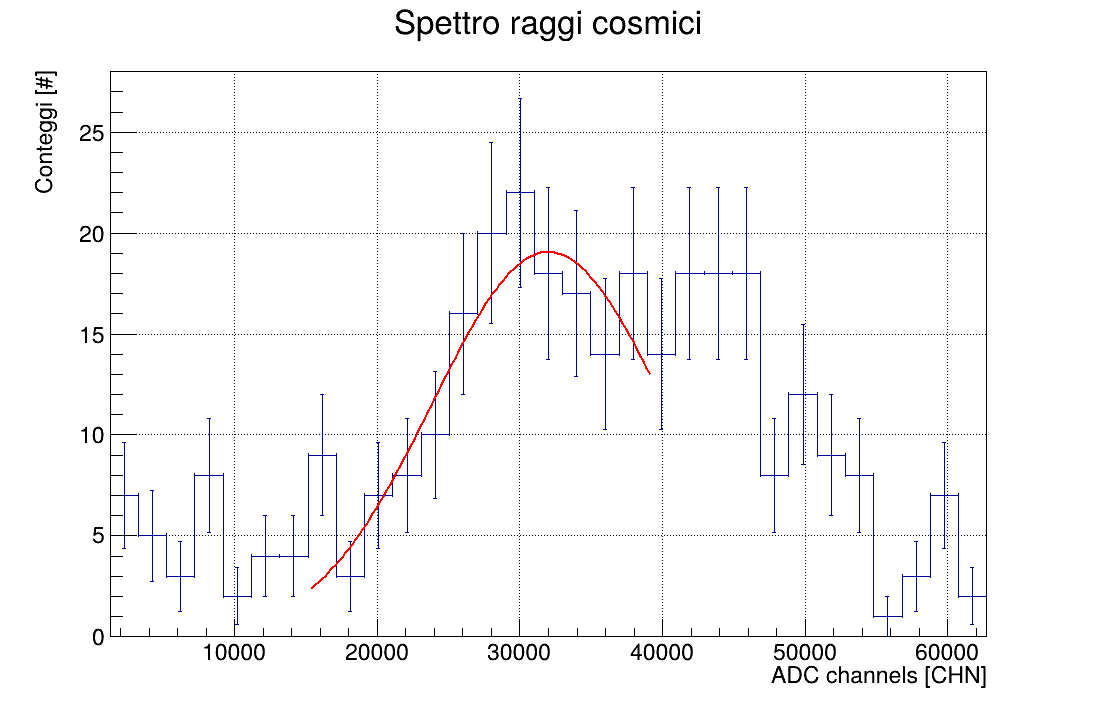
\includegraphics[width=0.65\linewidth]{fig2/raggi_zoom.png}
    \caption{ \footnotesize \footnotesize Istogramma di conteggi per numero di canale per i muoni cosmici con zoom sulla distribuzione di energia ($G_{ampl}=28$dB e $V_{bias}=54V$) e fit gaussiano: paramentri estratti $ \langle CHN\rangle = (32.0  \pm  1.6 )\cdot10^3\text{ CHN}$  e $ \sigma_{CHN} = ( 8.1 \pm 1.5 )\cdot10^3 \text{CHN}$, $\chi^2 =8$ e d.o.f.=9.}
    \label{fig:raggizoom}
\end{figure}
Dal fit gaussiano a sinistra del picco si estraggono valore medio e rispettiva deviazione standard, nonché la sua risoluzione: $$\langle \text{CHN} \rangle = ( 32  \pm  8  )\cdot10^3 \text{ CHN} $$ $$R_{CHN}= \frac{\sigma_\text{CHN}}{\langle\text{CHN}\rangle}= 0.25 \pm 0.05$$
Tramite il fattore di conversione $k_{Sr,eq}$, calcolato nella sezione 2.1.3, è possibile convertire $\langle \text{CHN} \rangle$ in energia depositata.
$$E_{DEP}=k_{Sr,eq}\cdot \langle CHN \rangle=( 1.6  \pm  0.5  ) \text{MeV}$$

\textit{Osservazione.} Come già accennato nella sezione 2.1.3, si utilizza $k_{eq}$ al posto di $k$ perché, nel caso dei raggi cosmici, le 
particelle non incidono sempre perpendicolarmente al rivelatore né attraversano per forza
il centro dello scintillatore. Al contrario, queste possono colpire la lastra in 
punti diversi e con angoli differenti, determinando una risposta del rivelatore 
che dipende dalla posizione di attraversamento.
Per tenere conto di questa non uniformità, si introduce quindi $k_{eq}$, che rappresenta il valore medio di $k$ nel caso in cui gli eventi siano distribuiti uniformemente su tutta la superficie dello scintillatore. \\

Infine, si verifica la legge di Bethe-Bloch per la perdita di energia, la quale prevede $$E_{DEP,att} = \frac{dE}{dx}x$$
dove $x$ è lo spessore dello scintillatore. 

Sapendo che $x=1\text{cm}$ e che per il polistirene si ha $\frac{dE}{dx}=2.06$ $\frac{MeV}{cm}$, si ottiene un valore atteso
$$E_{DEP,att} = 2.06 MeV $$ il quale risulta statisticamente compatibile con la stima sperimentale $E_{DEP}$.

\newpage
{\color{gray}\hrule}
\begin{center}
\section{Conclusioni}
\bigskip
\end{center}
{\color{gray}\hrule}
\vspace{0.5cm}
Nella prima parte dell'esperienza si è caratterizzato il comportamento di un \textit{Silicon Photomultiplier}, stimandone in particolare il \textit{dark count rate} e l'\textit{optical crosstalk}: si è anche verificato (seppur con dei valori di $\chi^2$ bassi) che il DCR segue un andamento lineare crescente al variare della temperatura di funzionamento, mentre l'OCT rimane pressochè costante.

Utilizzando una sorgente LED, si è prima stimato il guadagno del SiPM e si è poi studiata la risposta dell'apparato di misura, composto da una \textit{Power Supply and Amplification Unit} e da un \textit{Digitizer}, al variare di diverse impostazioni del setup sperimentale: con la relazione lineare tra il \textit{gain} digitale $G_{ampl}$ e la distanza tra i picchi $\Delta_{pp}$, si è dimostrato che l'apparato risponde linearmente alla quantità di carica restituita dall'accensione delle celle del SiPM; mentre con la relazione lineare tra la tensione di alimentazione $V_{bias}$ e il guadagno del SiPM si è verificato che la risposta del SiPM all'aumentare della tensione di polarizzazione inversa delle celle è lineare. Si è infine stimato il numero medio di celle accese al variare dell'intensità del LED in modo approssimativo, mentre non è stato possibile stimarlo con il metodo più accurato.

Nella seconda parte dell'esperienza si è utilizzato il SiPM per studiare il decadimento $\beta^-$ dello ${}^{90}$Sr: si è estrapolato con la tecnica del plot di Kurie l'\textit{end point} $T_{0,Y}$ dello spettro per stimare il coefficiente di conversione tra le misure in CHN e il loro valore in energia (sia per sorgenti allineate sia per sorgenti non allineate al SiPM) e lo si è usato per stimare il massimo della distribuzione $T_{max,\text{Sr}}$. Si è poi studiato l'assorbimento della radiazione $\beta^-$ in foglietti di carta e alluminio, ricavando da un lato il valore del coefficiente di assorbimento della carta, il quale risulta nel range di valore atteso, e dall'altro stimando lo spessore dei foglietti di alluminio (di difficile misura diretta) conoscendone il coefficiente di assorbimento.

%paolo dimmi se ti sembra grammaticalmente corretto e se ha senso 
Si è poi considerato lo spettro del ${}^{137}$Cs, dove tramite l'analisi dei picchi a bassi canali si è stimata la risoluzione attesa dell'apparato, la quale risulta statisticamente compatibile con quella ricavata dal picco di conversione interna. Si è infine stimato il valore massimo della distribuzione $T_{max,\text{Cs}}$, che non risulta compatibile con il valore atteso per una sottostima dell'errore.

Con l'utilizzo della \textit{Cosmic Box} è stato possibile acquisire uno spettro e stimare l'energia in media depositata dai muoni nello scintillatore. 
Tale valore è risultato statisticamente compatibile con la previsione teorica della legge di Bethe-Bloch. La risoluzione dell'apparato ottenuta dallo spettro dei muoni risulta maggiore di quella ottenuta dallo studio dello spettro del ${}^{137}$Cs. Si attribuisce questo aumento in primo luogo al piccolo numero di eventi registrati e in secondo luogo al fatto che è stato possibile effettuare una regressione solo sulla coda sinistra dei dati e non sulla coda destra poiché questa è influenzata dai muoni fuori asse.

\newpage
{\color{gray}\hrule}
\begin{center}
\section{Appendice}
\addtocontents{toc}{\setcounter{tocdepth}{0}}
\bigskip
\end{center}
{\color{gray}\hrule}
\vspace{0.5cm}
\subsection{Caratterizzazione di un SiPM senza sorgente luminosa}
Vengono qui riportati gli istogrammi relaitivi alla sezione 1.1.2 con i relativi fit gaussiani
\begin{multicols}{2}
%1111111111111111111111111111
\begin{figure}[H]
    \centering
    
\includegraphics[width=0.99\linewidth]{appendice/dcr_l19.png}
    \caption{\footnotesize $\chi^2=5$, d.o.f.$=6$}
    % 
\end{figure}

\begin{figure}[H]
    \centering
    
\includegraphics[width=0.99\linewidth]{appendice/dcr_h19.png}
    \caption{\footnotesize $\chi^2=5$, d.o.f.$=7$}
    % 
\end{figure}
\end{multicols}
\begin{multicols}{2}
%222222222222222222222222222222222222
\begin{figure}[H]
    \centering
    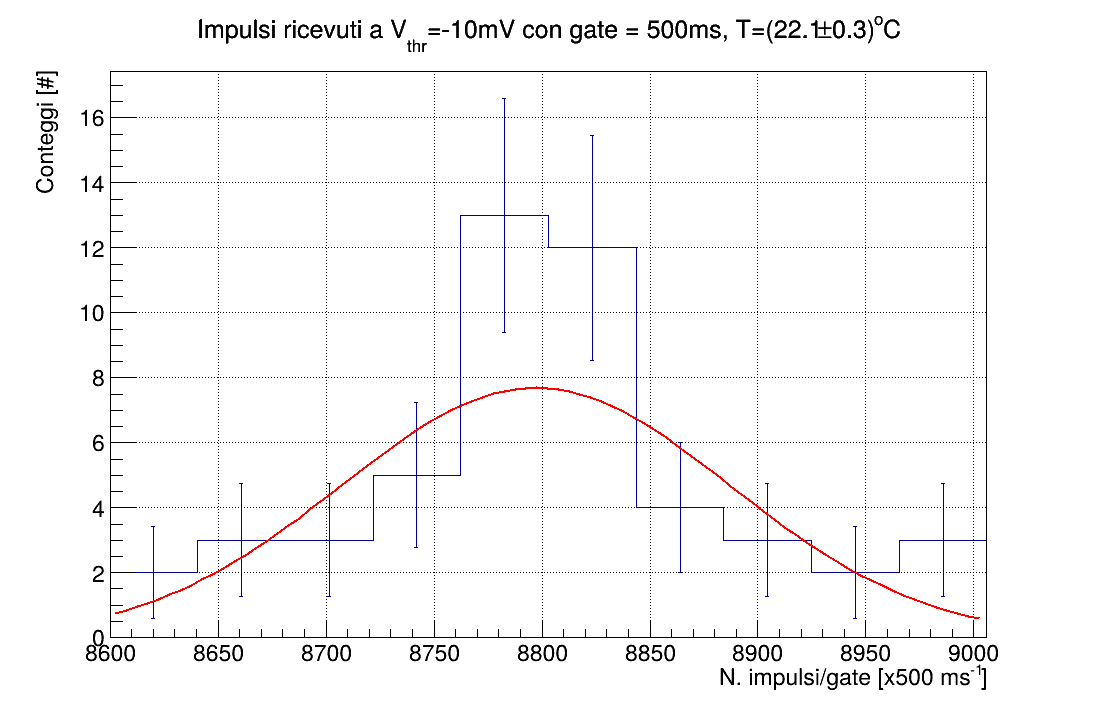
\includegraphics[width=0.99\linewidth]{appendice/dcr_l21.png}
    \caption{\footnotesize $\chi^2=8$, d.o.f.$=7$}
    % 
\end{figure}

\begin{figure}[H]
    \centering
    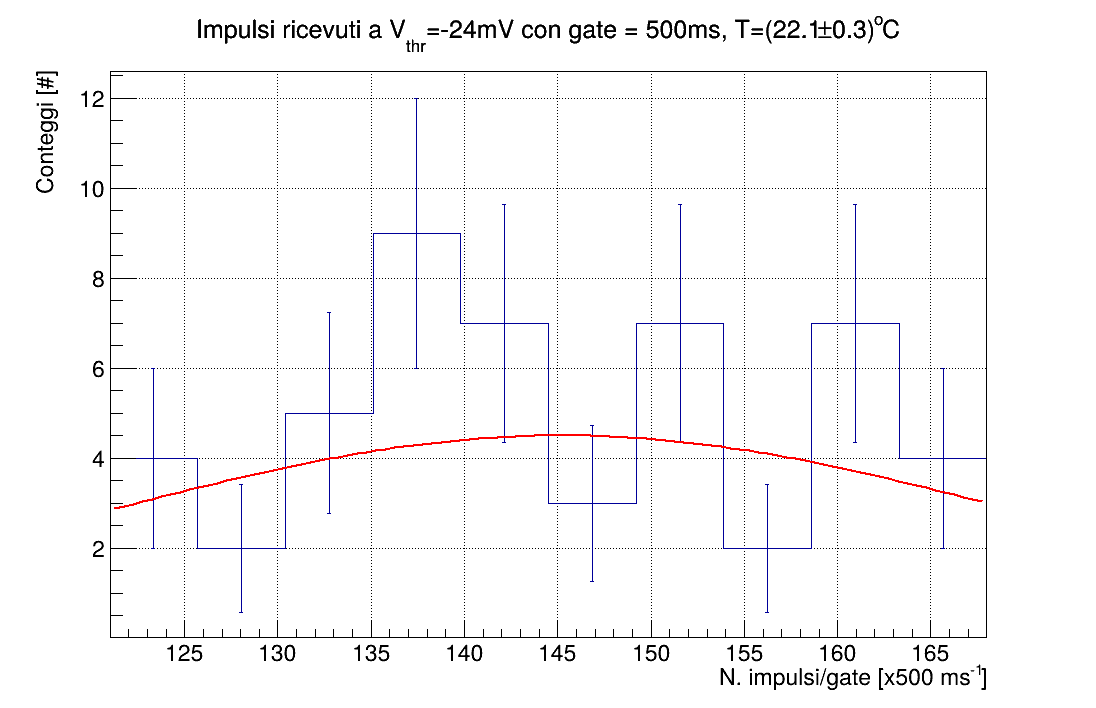
\includegraphics[width=0.99\linewidth]{appendice/dcr_h21.png}
    \caption{\footnotesize $\chi^2=10$, d.o.f.$=7$}
    % 
\end{figure}
\end{multicols}
\begin{multicols}{2}
%33333333333333333333333333333333333333
\begin{figure}[H]
    \centering
    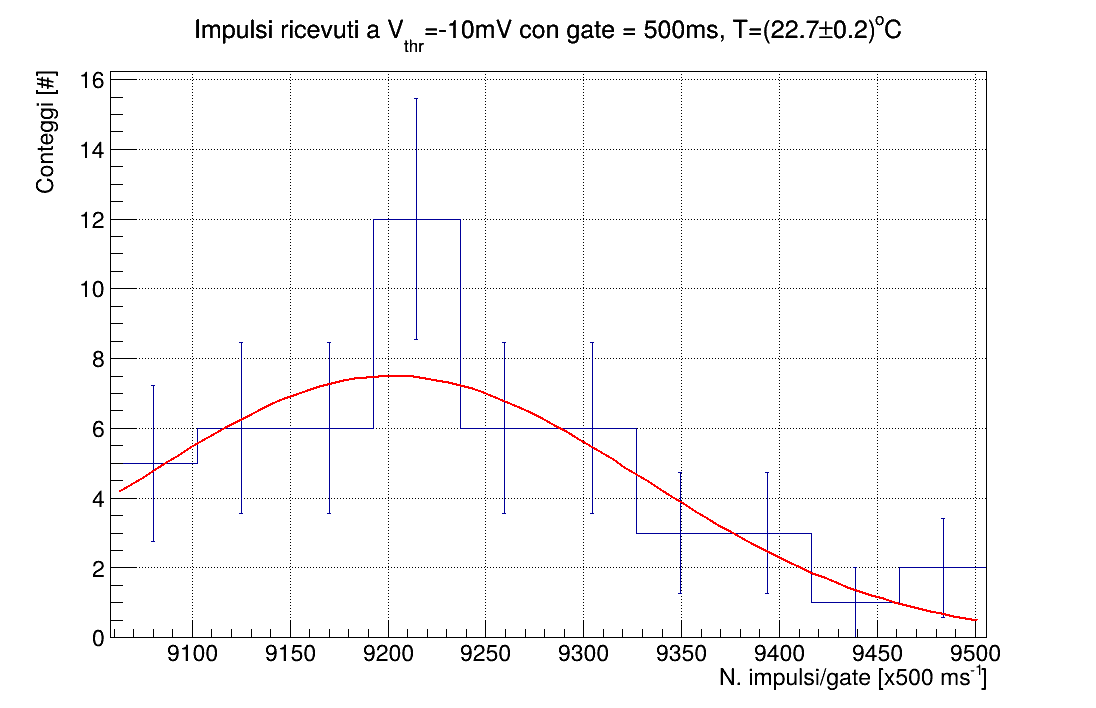
\includegraphics[width=0.99\linewidth]{appendice/dcr_l22.png}
    \caption{\footnotesize $\chi^2=4$, d.o.f.$=7$}
    % 
\end{figure}

\begin{figure}[H]
    \centering
    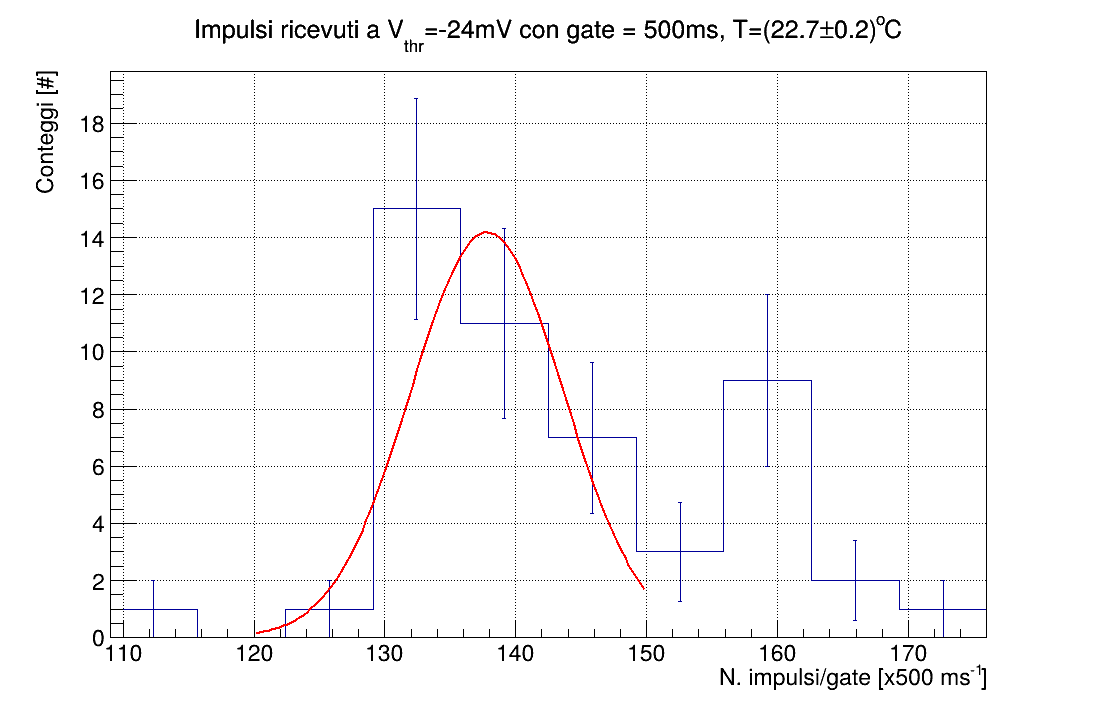
\includegraphics[width=0.99\linewidth]{appendice/dcr_h22.png}
    \caption{\footnotesize $\chi^2=4$, d.o.f.$=1$}
     
\end{figure}
\end{multicols}
\begin{multicols}{2}
%4444444444444444444444444444444444444444444
\begin{figure}[H]
    \centering
    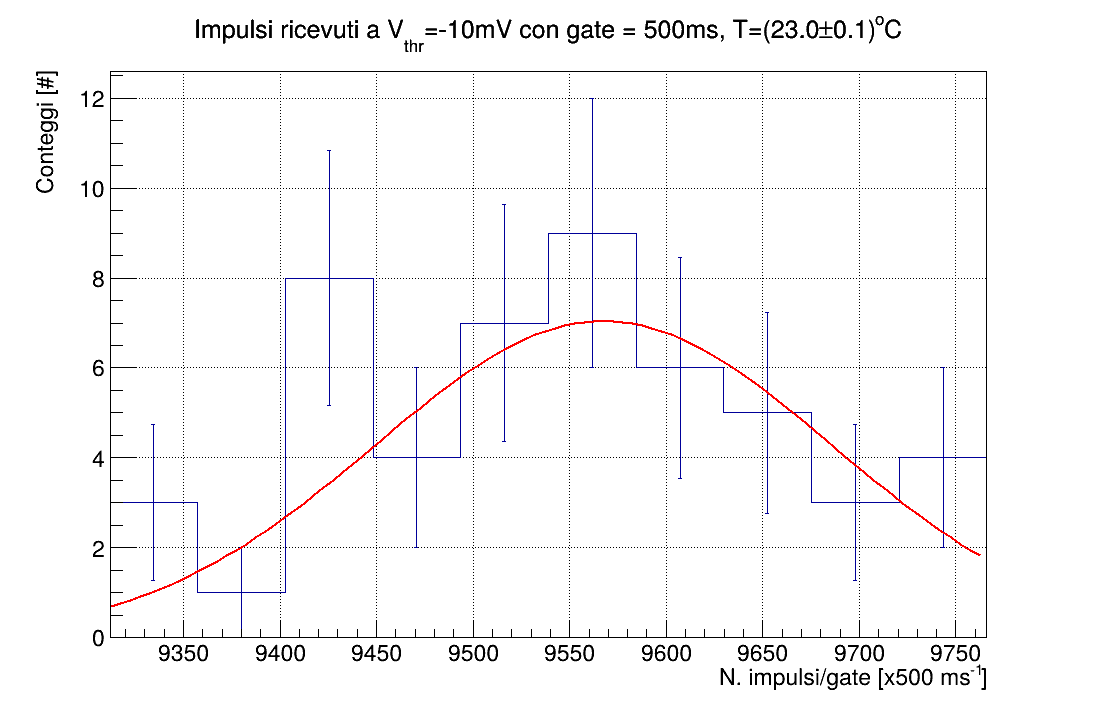
\includegraphics[width=0.99\linewidth]{appendice/dcr_l23.png}
    \caption{\footnotesize $\chi^2=7$, d.o.f.$=7$}
     
\end{figure}

\begin{figure}[H]
    \centering
    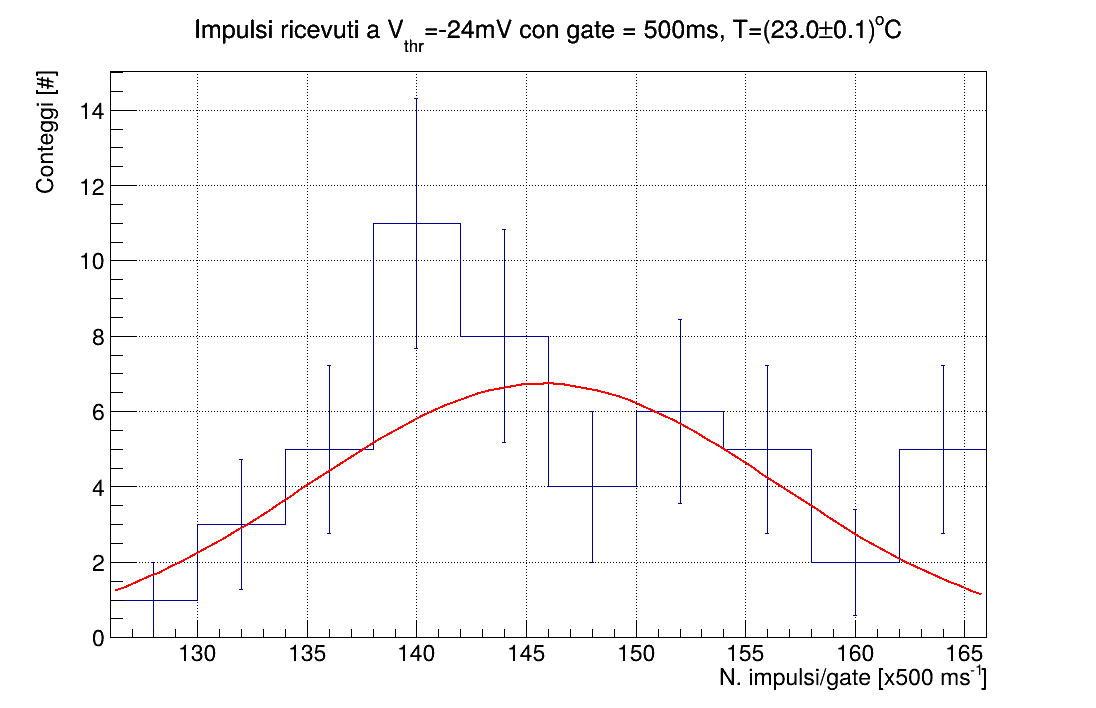
\includegraphics[width=0.99\linewidth]{appendice/dcr_h23.png}
    \caption{\footnotesize $\chi^2=8$, d.o.f.$=7$}
     
\end{figure}
\end{multicols}
\begin{multicols}{2}
%555555555555555555555555555555555555555555555
\begin{figure}[H]
    \centering
    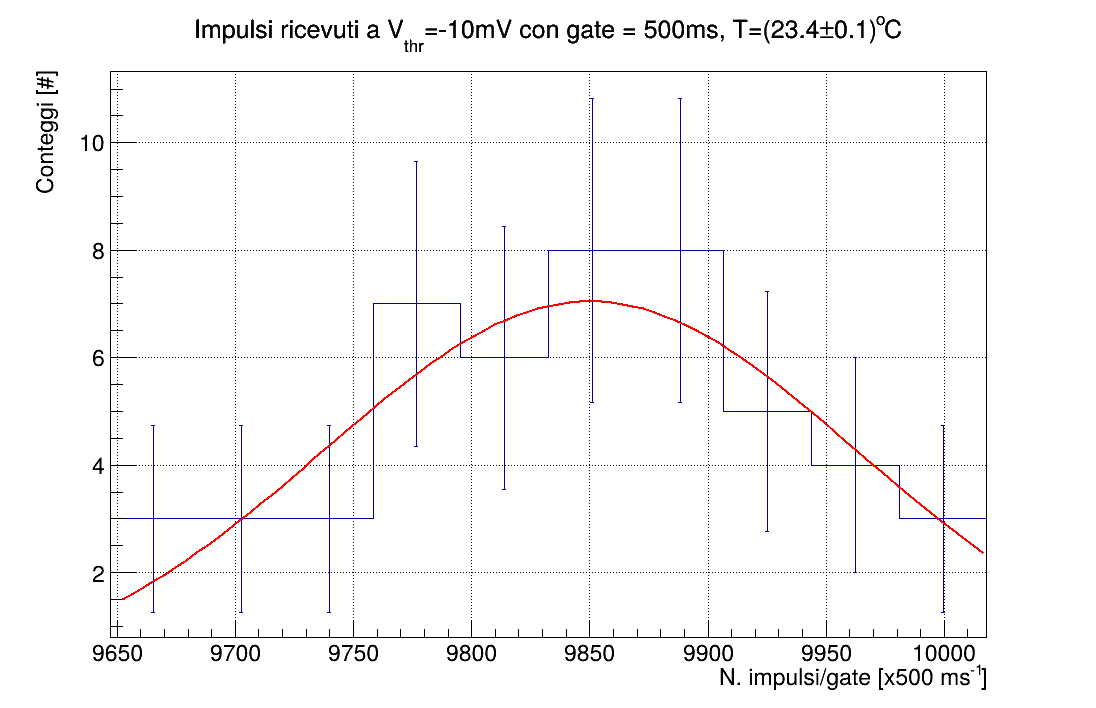
\includegraphics[width=0.99\linewidth]{appendice/dcr_l23_3.png}
    \caption{\footnotesize $\chi^2=2$, d.o.f.$=7$}
     
\end{figure}

\begin{figure}[H]
    \centering
    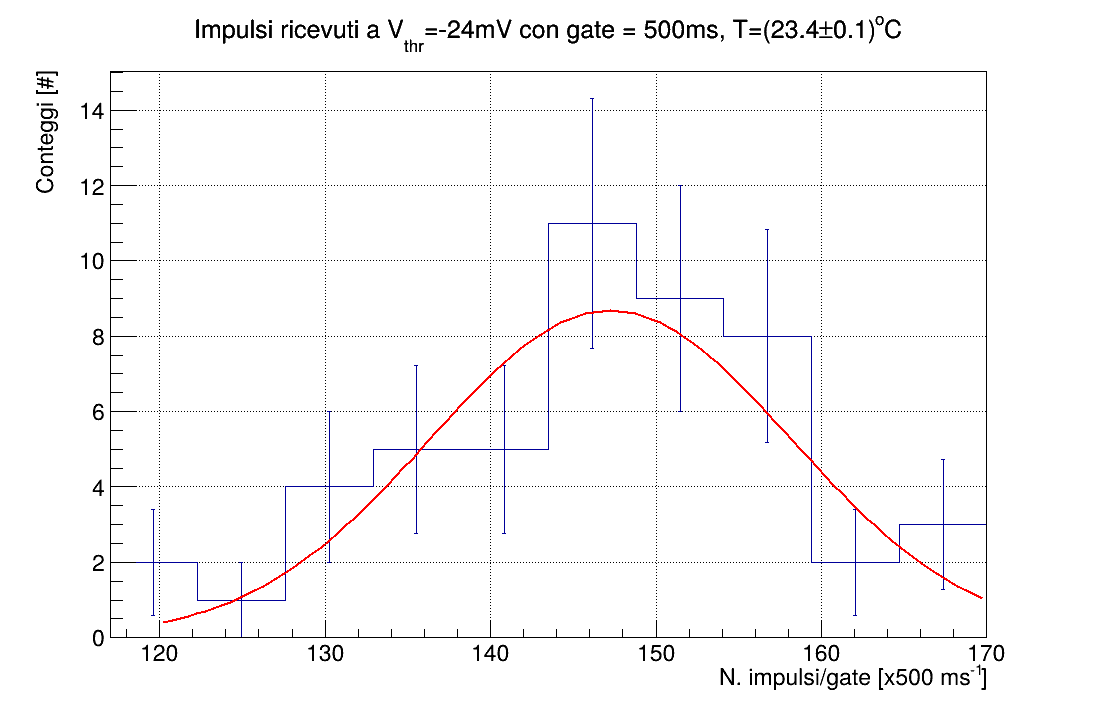
\includegraphics[width=0.99\linewidth]{appendice/dcr_h23_3.png}
    \caption{\footnotesize $\chi^2=4$, d.o.f.$=6$}
     
\end{figure}
\end{multicols}
\begin{multicols}{2}
%66666666666666666666666666666666666666666666666
\begin{figure}[H]
    \centering
    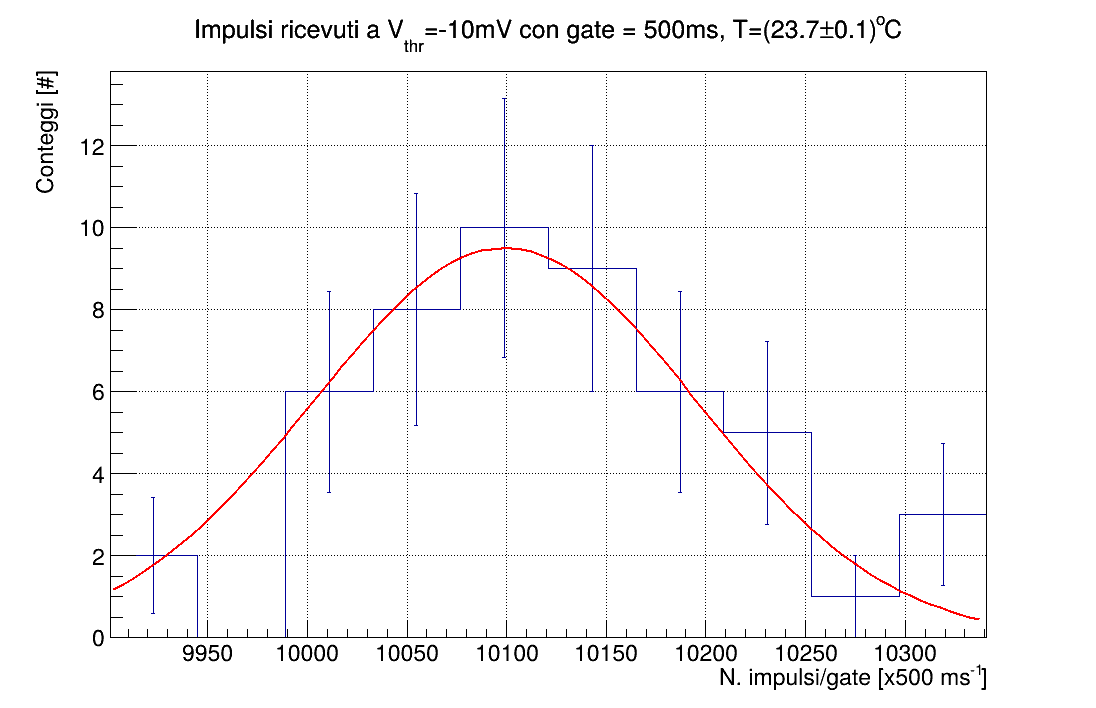
\includegraphics[width=0.99\linewidth]{appendice/dcr_l23_6.png}
    \caption{\footnotesize $\chi^2=3$, d.o.f.$=6$}
     
\end{figure}

\begin{figure}[H]
    \centering
    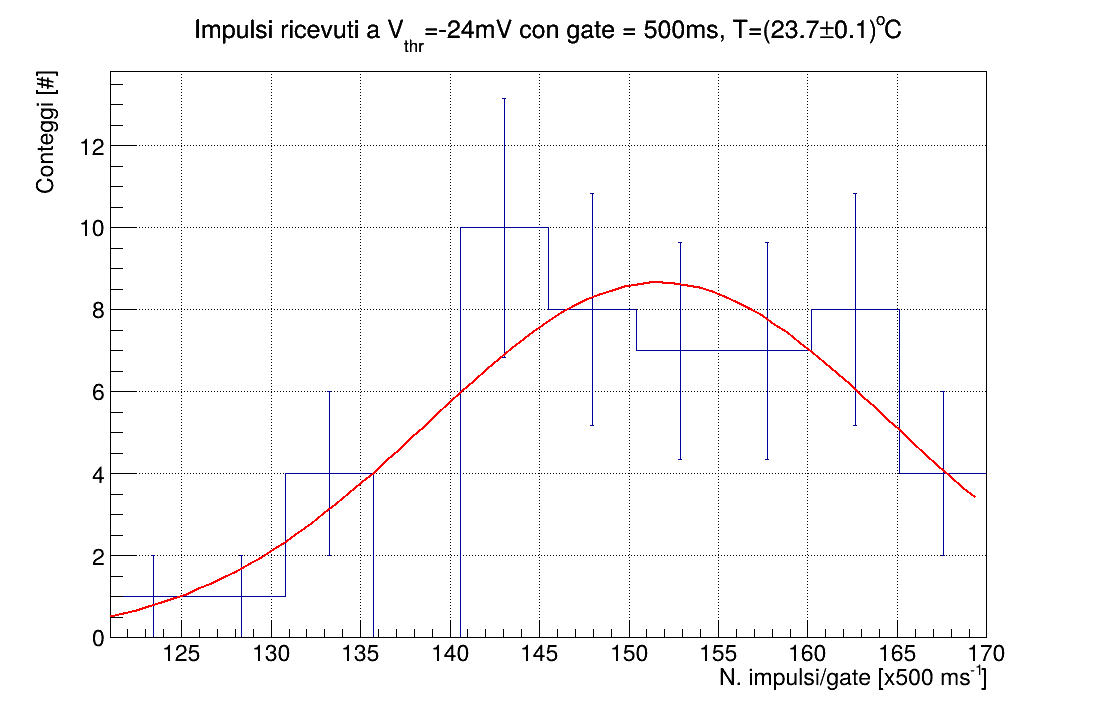
\includegraphics[width=0.99\linewidth]{appendice/dcr_h23_6.png}
    \caption{\footnotesize $\chi^2=3$, d.o.f.$=6$}
     
\end{figure}
\end{multicols}
\newpage
\begin{multicols}{2}
%777777777777777777777777777777777777777777777777
\begin{figure}[H]
    \centering
    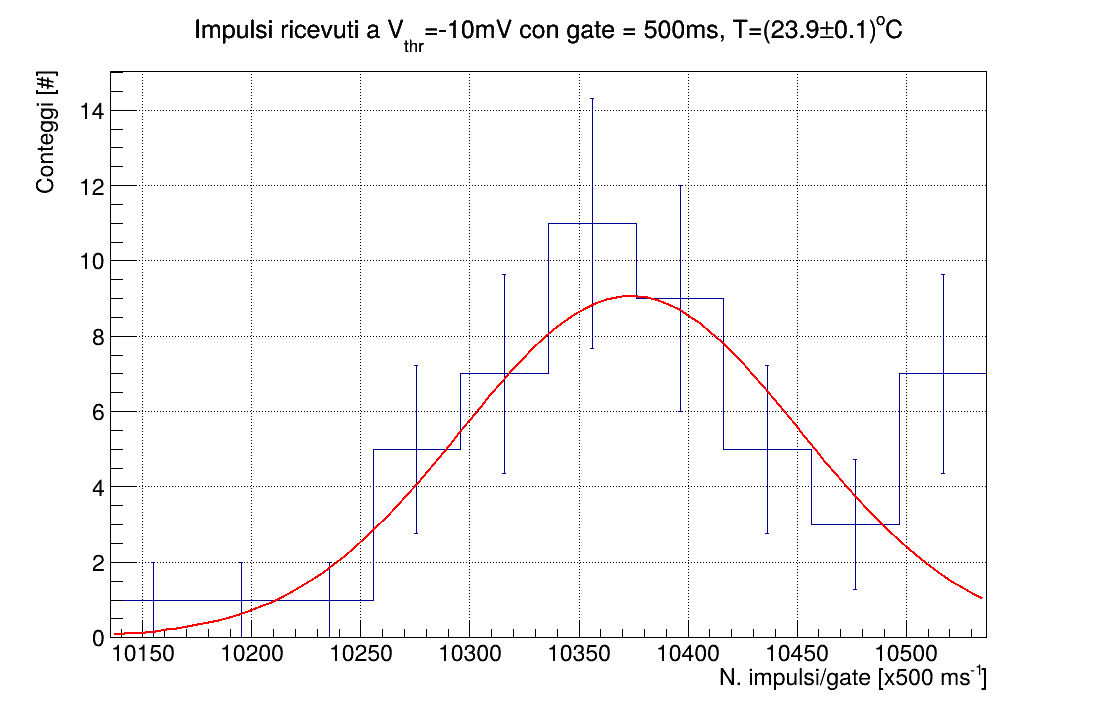
\includegraphics[width=0.99\linewidth]{appendice/dcr_l23_9.png}
    \caption{\footnotesize $\chi^2=7$, d.o.f.$=7$}
     
\end{figure}

\begin{figure}[H]
    \centering
    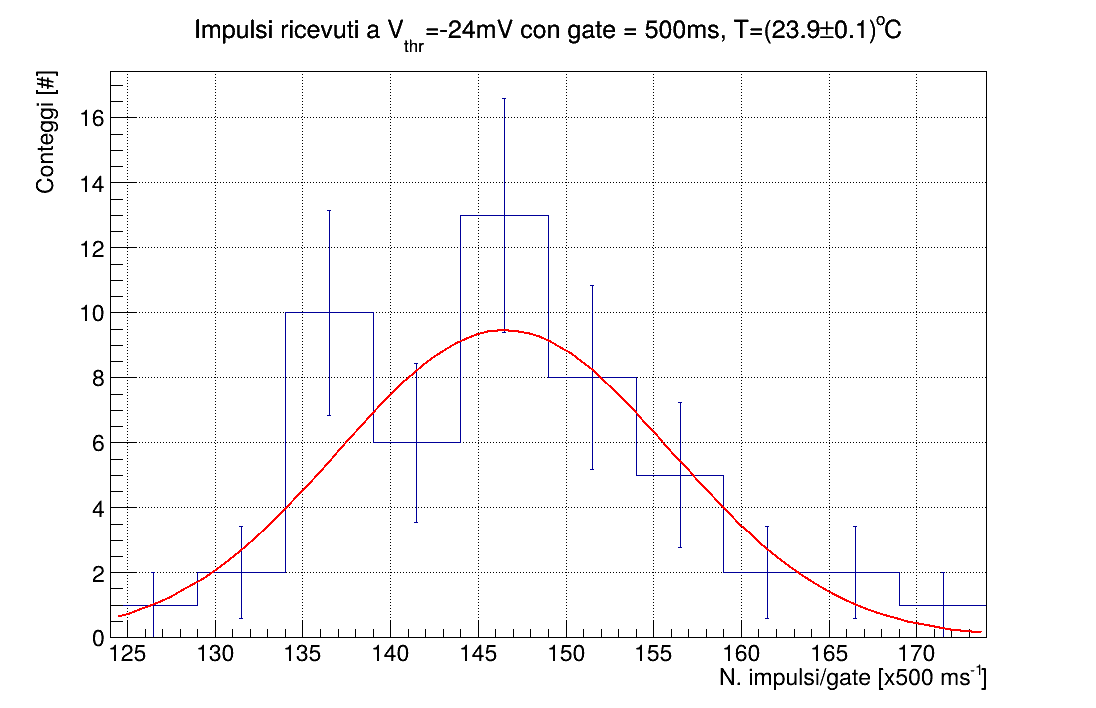
\includegraphics[width=0.99\linewidth]{appendice/dcr_h23_9.png}
    \caption{\footnotesize $\chi^2=5$, d.o.f.$=7$}
     
\end{figure}
\end{multicols}

\subsection{Caratterizzazione di un SiPM con sorgente luminosa (LED)}
\subsubsection{Stima di $G_{SiPM}$}
Si riportano qui i valori dei picchi della sezione 1.2.1, le loro incertezze e le stime di $\Delta_{pp}$.

\begin{table}[H]
    \centering
    \begin{tabular}{|c|c|c|c|c|}
        \hline
        
        \textbf{N. picco} & \textbf{$\mathbf{\chi^2}$ fit} & \textbf{d.o.f.} &$\mathbf{(p_i\pm\sigma_{p,i})}$\textbf{[CHN]} & $\mathbf{\Delta_{pp}}$\textbf{[CHN]} \\ \hline
        
        0   & 27 & 27 & $1\pm8$ & \textbf{X} \\ \hline
        1   & 40 & 52 & $233\pm12$    & $232\pm15$ \\ \hline
        2   & 72 & 71 & $463\pm17$    & $230\pm20$ \\ \hline        
        3   & 100 & 82 & $690\pm20$   & $230\pm30$ \\ \hline
        4   & 96 & 97 & $920\pm30$    & $230\pm40$ \\ \hline
        5   & 141 & 117 & $1150\pm40$ & $230\pm50$ \\ \hline
    \end{tabular}
    \caption{\footnotesize Coordinate dei picchi, parametri dei fit e stime di $\Delta_{pp}$ utilizzate per il calcolo di $G_{SiPM}$.}
    \label{tab:gsipm}   
\end{table}
\subsubsection{$\Delta_{pp}$ in funzione di $G_{ampl}$}
\label{sec:app_gain}
Si riportano qui gli spettri del LED al variare di $G_{ampl}$, usati nella sezione 1.2.2.
\begin{multicols}{2}
    \begin{figure}[H]
    \centering
    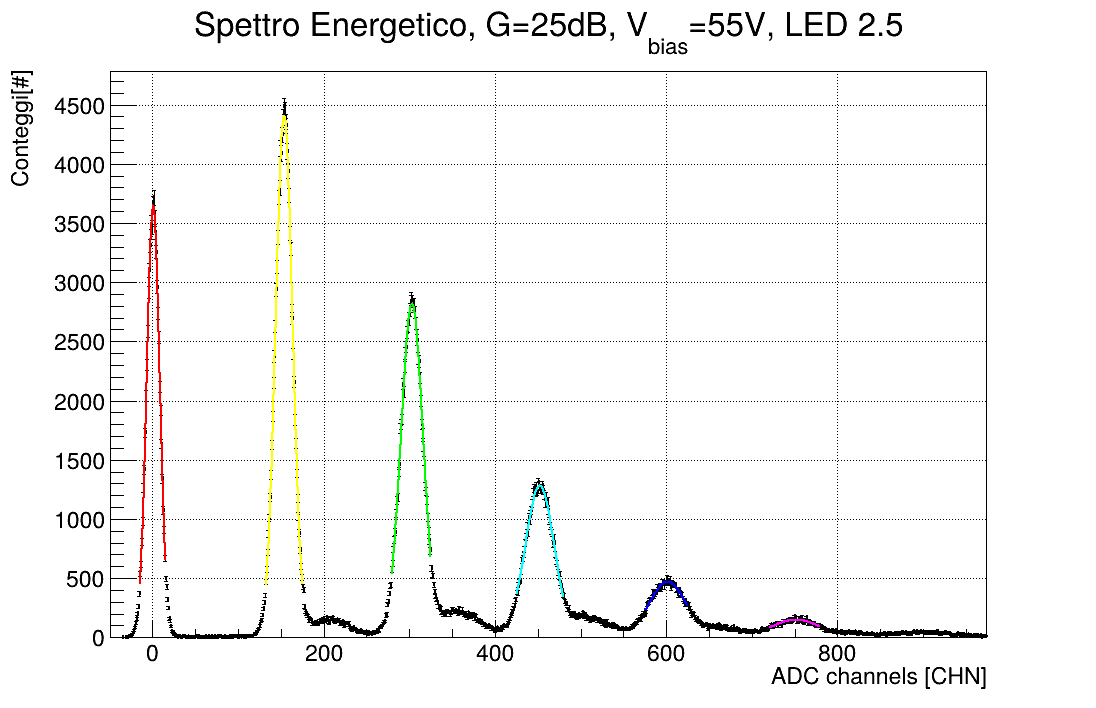
\includegraphics[width=0.99\linewidth]{appendice/gain25.png}
     
\end{figure}
\begin{figure}[H]
    \centering
    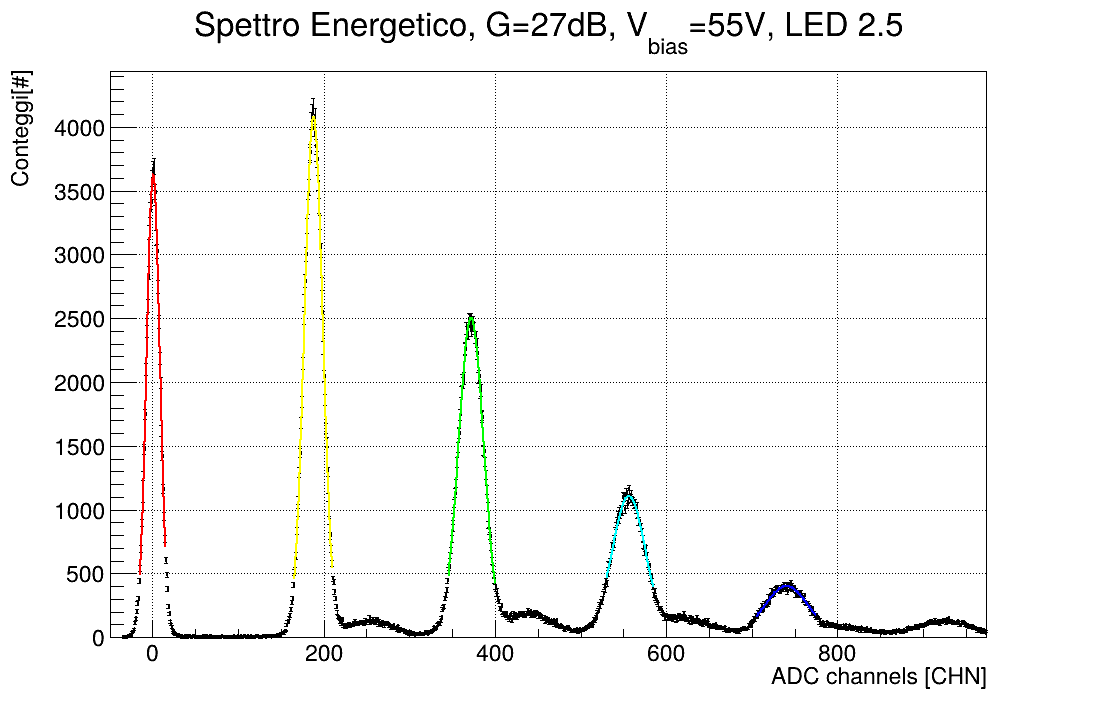
\includegraphics[width=0.99\linewidth]{appendice/gain27.png}
     
\end{figure}
\end{multicols}
\newpage
\begin{multicols}{2}
    \begin{figure}[H]
    \centering
    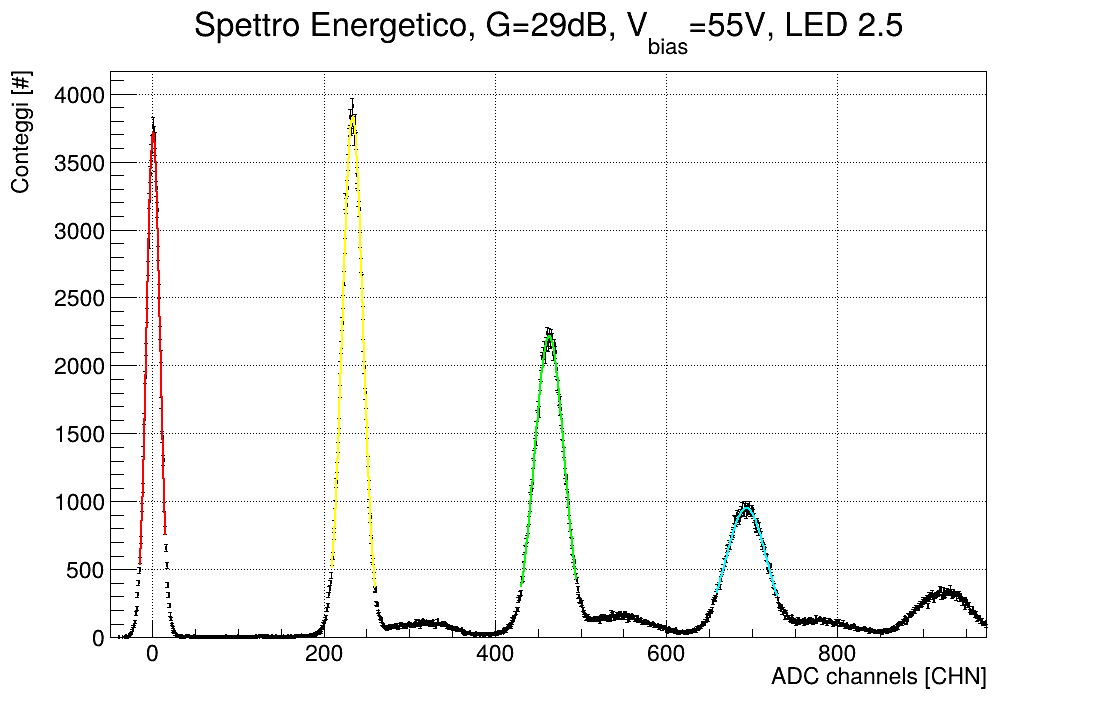
\includegraphics[width=0.99\linewidth]{appendice/gain29.png}
     
\end{figure}
\begin{figure}[H]
    \centering
    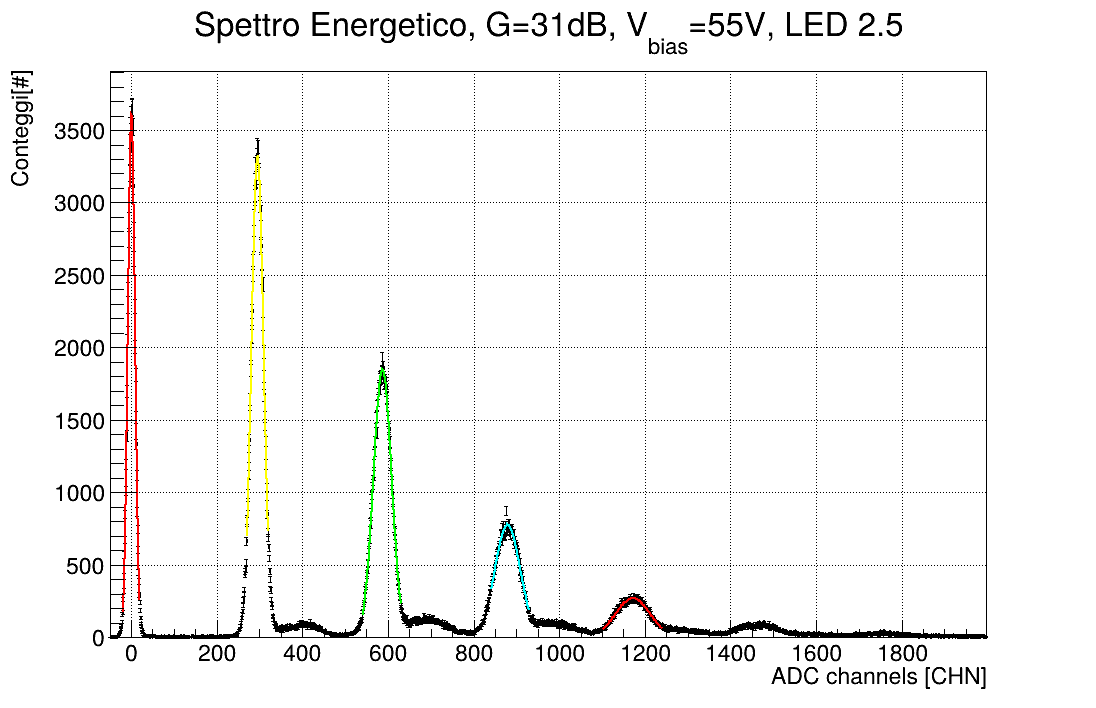
\includegraphics[width=0.99\linewidth]{appendice/gain31.png}
     
\end{figure}
\end{multicols}

\begin{multicols}{2}
    \begin{figure}[H]
    \centering
    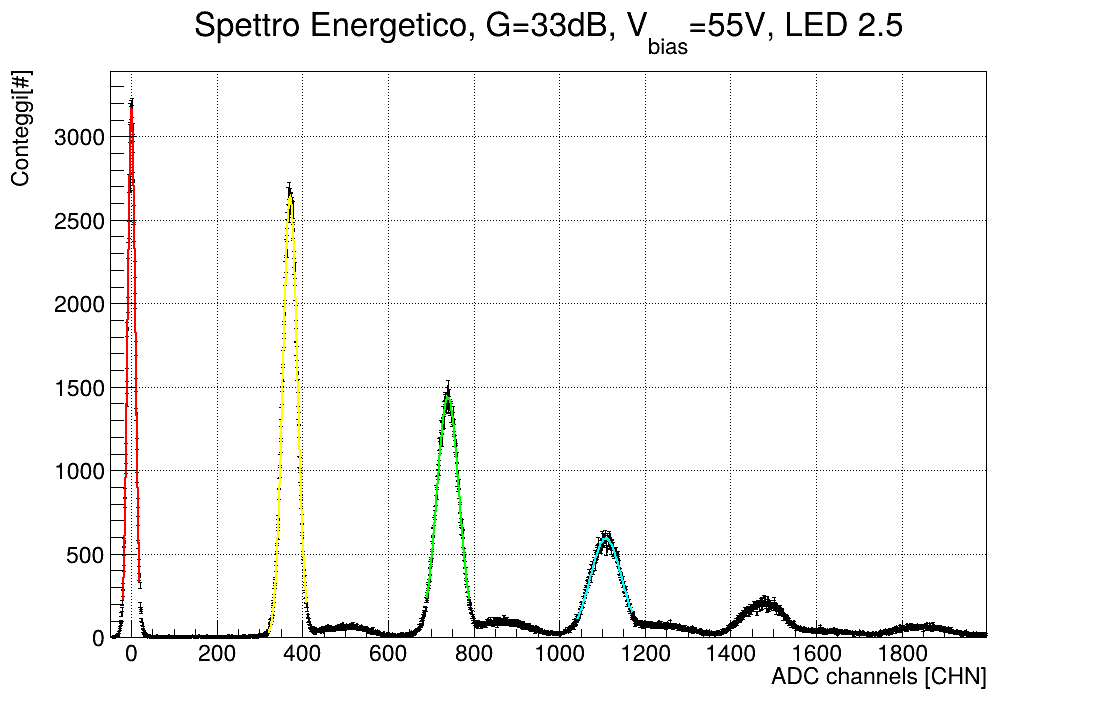
\includegraphics[width=0.99\linewidth]{appendice/gain33.png}
     
\end{figure}
\begin{figure}[H]
    \centering
    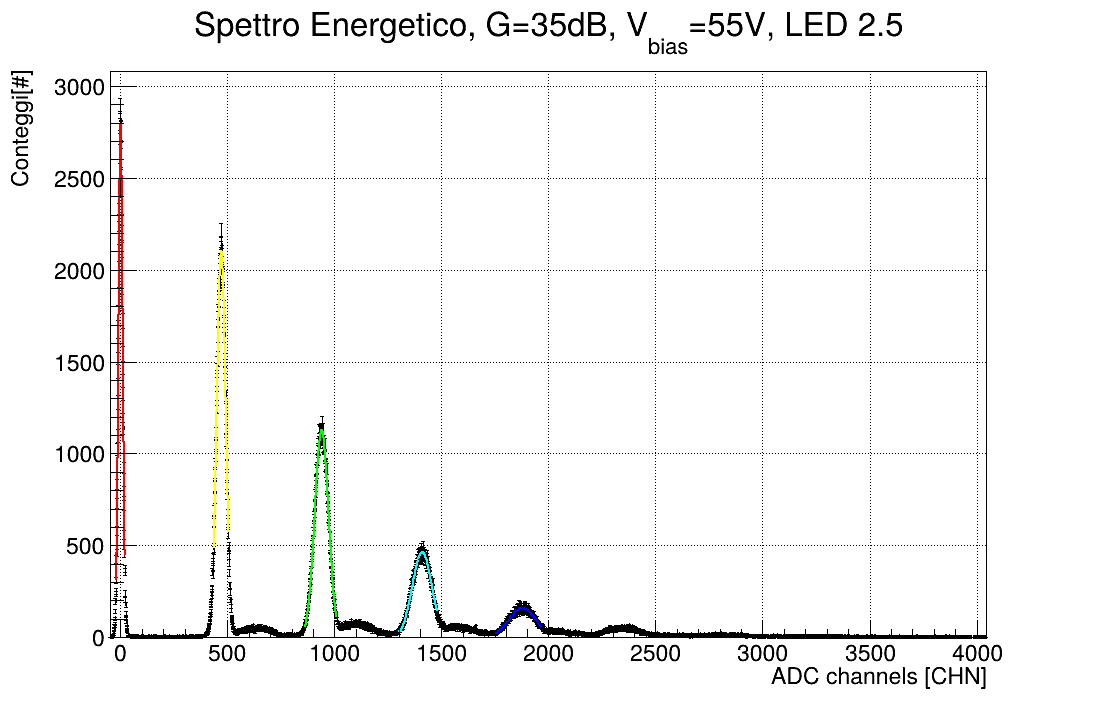
\includegraphics[width=0.99\linewidth]{appendice/gain35.png}
     
\end{figure}
\end{multicols}
\subsubsection{$G_{SiPM}$ in funzione di $V_{bias}$}
Si riportano qui gli spettri del LED al variare di $V_{bias}$, usati nella sezione 1.2.3.
\begin{multicols}{2}
    \begin{figure}[H]
    \centering
    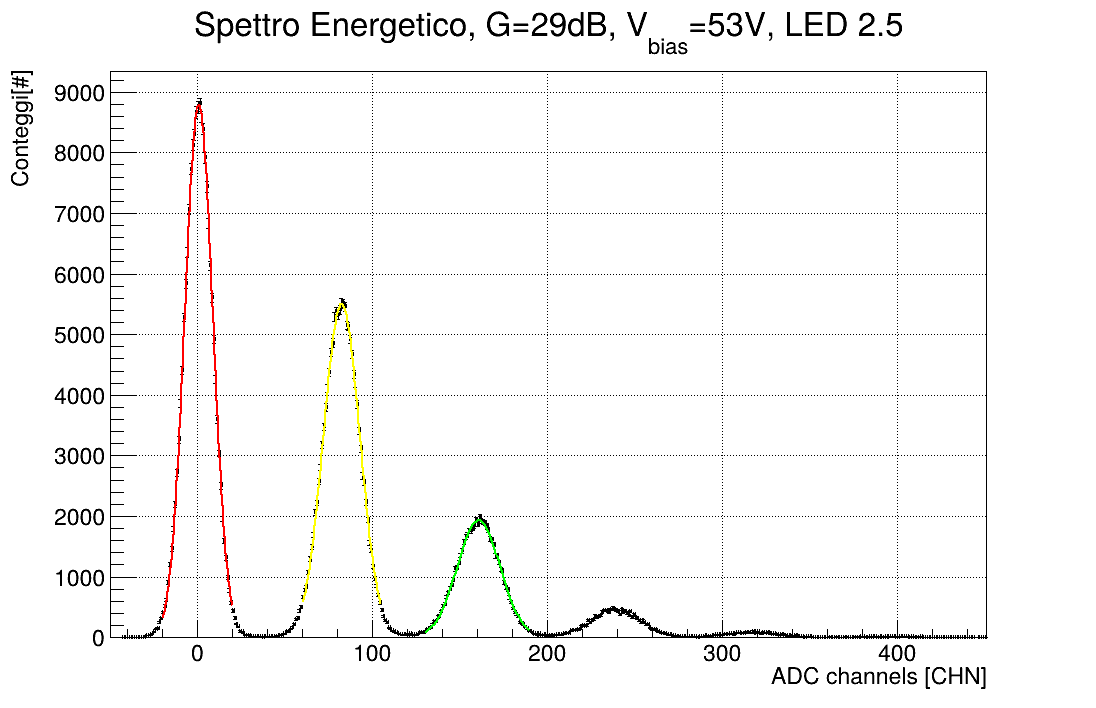
\includegraphics[width=0.99\linewidth]{appendice/V53.png}
     
\end{figure}
\begin{figure}[H]
    \centering
    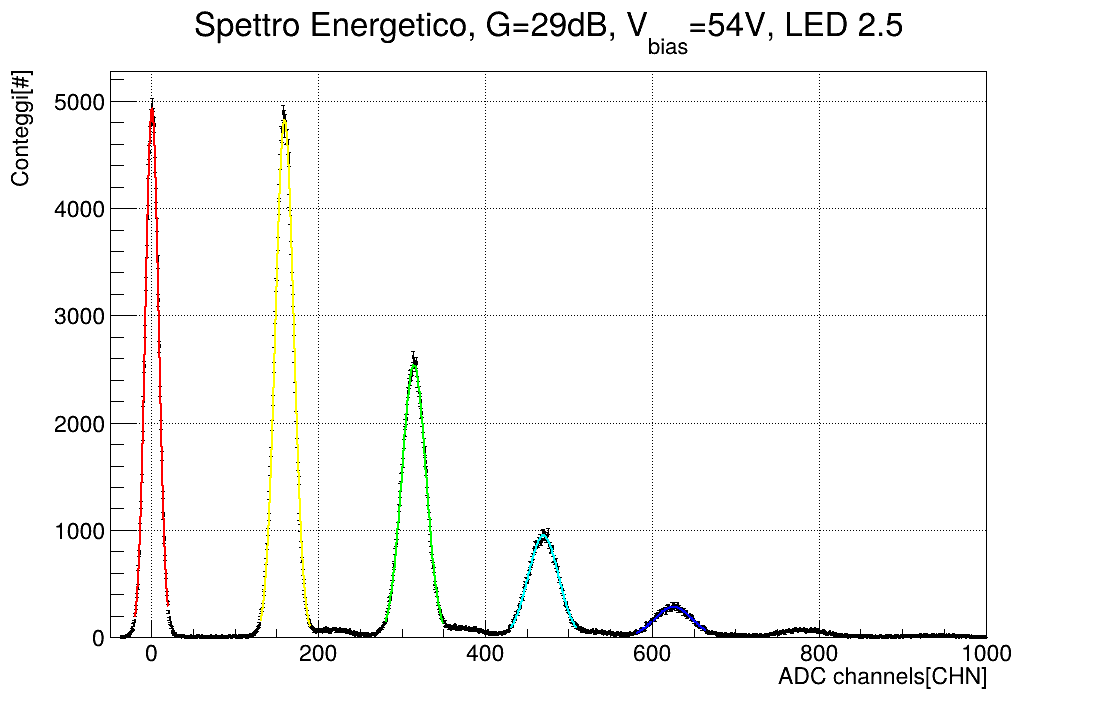
\includegraphics[width=0.99\linewidth]{appendice/V54.png}
     
\end{figure}
\end{multicols}
\newpage
\begin{multicols}{2}
    \begin{figure}[H]
    \centering
    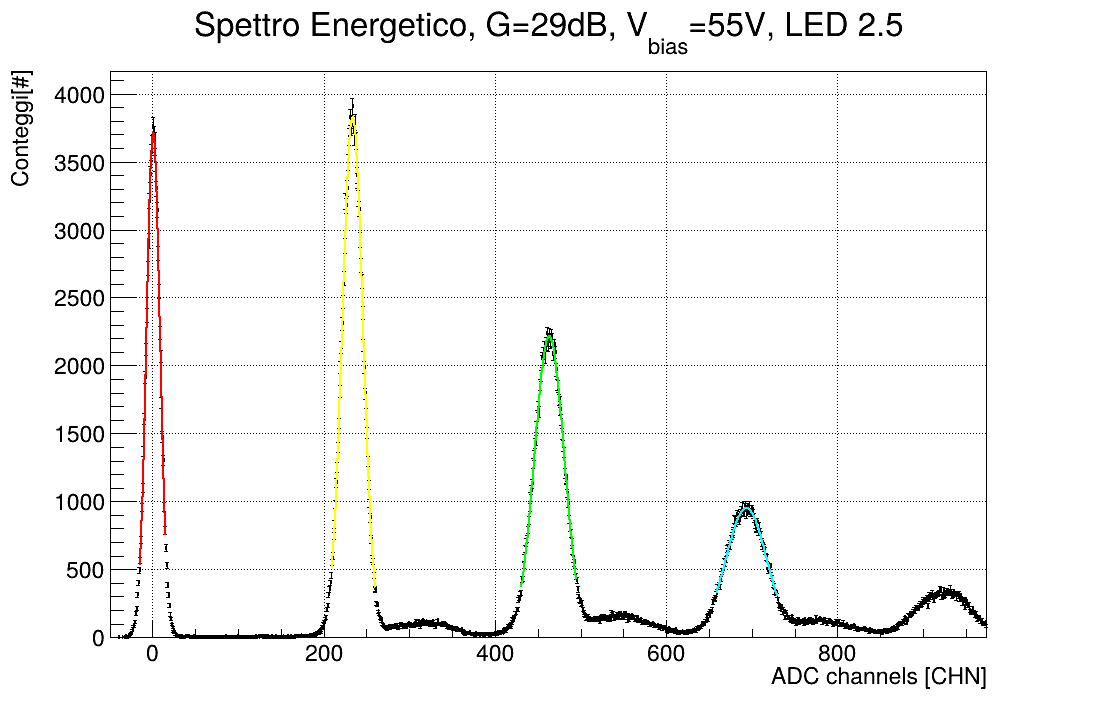
\includegraphics[width=0.99\linewidth]{appendice/V55.png}
     
\end{figure}
\begin{figure}[H]
    \centering
    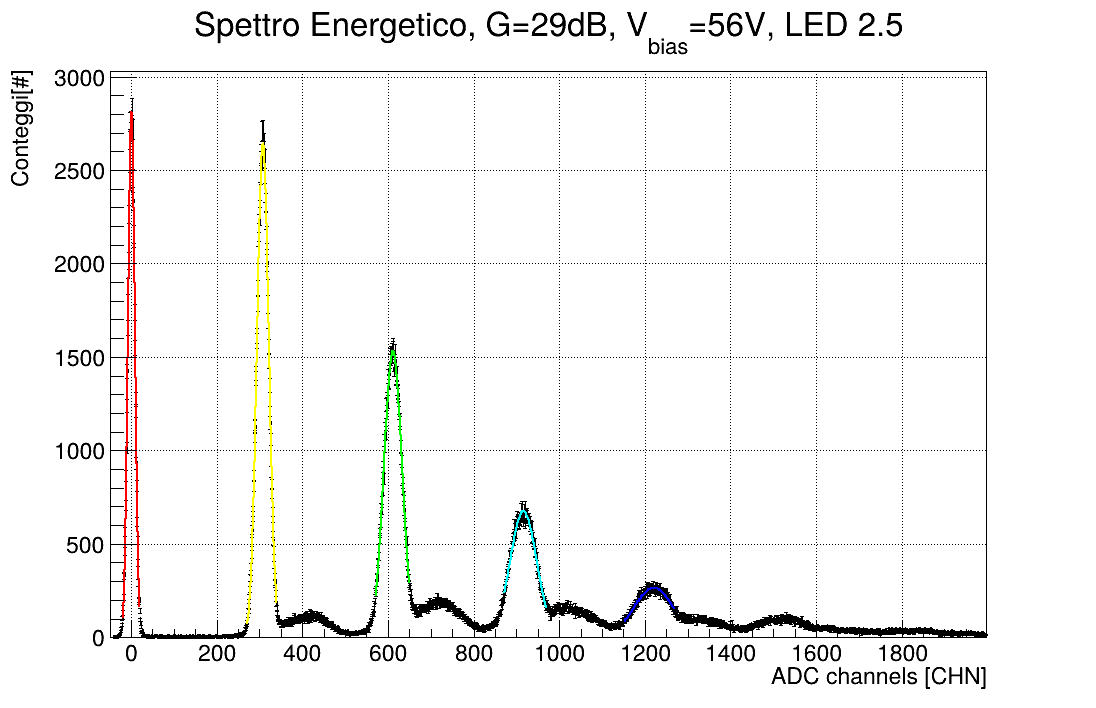
\includegraphics[width=0.99\linewidth]{appendice/V56.png}
     
\end{figure}
\end{multicols}
\begin{multicols}{2}
\begin{figure}[H]
    \centering
    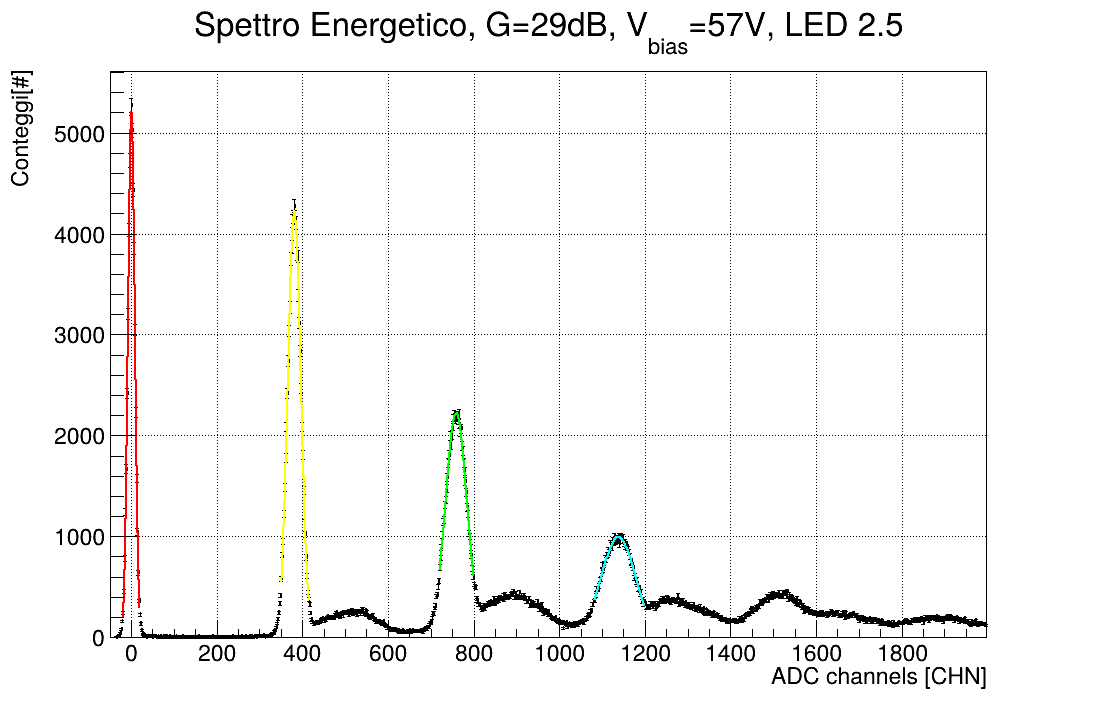
\includegraphics[width=0.99\linewidth]{appendice/V57.png}
     
\end{figure}
\end{multicols}
\subsubsection{Stima del numero di fotoni rivelati}

Si riportano qui i valori dei picchi della sezione 1.2.4 ($I_{LED} = 2.5$), le loro incertezze e le stime di $\Delta_{pp}$.

\begin{table}[H]
    \centering
    \begin{tabular}{|c|c|c|c|c|}
        \hline
        
        \textbf{N. picco} & \textbf{$\mathbf{\chi^2}$ fit} & \textbf{d.o.f.} &$\mathbf{(p_i\pm\sigma_{p,i})}$\textbf{[CHN]} & $\mathbf{\Delta_{pp}}$\textbf{[CHN]} \\ \hline
        
        0   & 46 & 37 & $1\pm8$ & \textbf{X} \\ \hline
        1   & 65 & 52 & $234\pm12$    & $232\pm15$ \\ \hline
        2   & 67 & 72 & $463\pm17$    & $230\pm20$ \\ \hline        
        3   & 71 & 77 & $690\pm20$   & $230\pm30$ \\ \hline
    \end{tabular}
    \caption{\footnotesize Coordinate dei picchi, parametri dei fit e stime di $\Delta_{pp}$ utilizzate per il calcolo di $\mu_{ph}$ a $I_{LED} = 2.5$}
    \label{tab:led2_5}   
\end{table}
\newpage
Si riportano gli spettri con $I_{LED} = 2.0$ e $2.8$
\begin{multicols}{2}
    \begin{figure}[H]
    \centering
    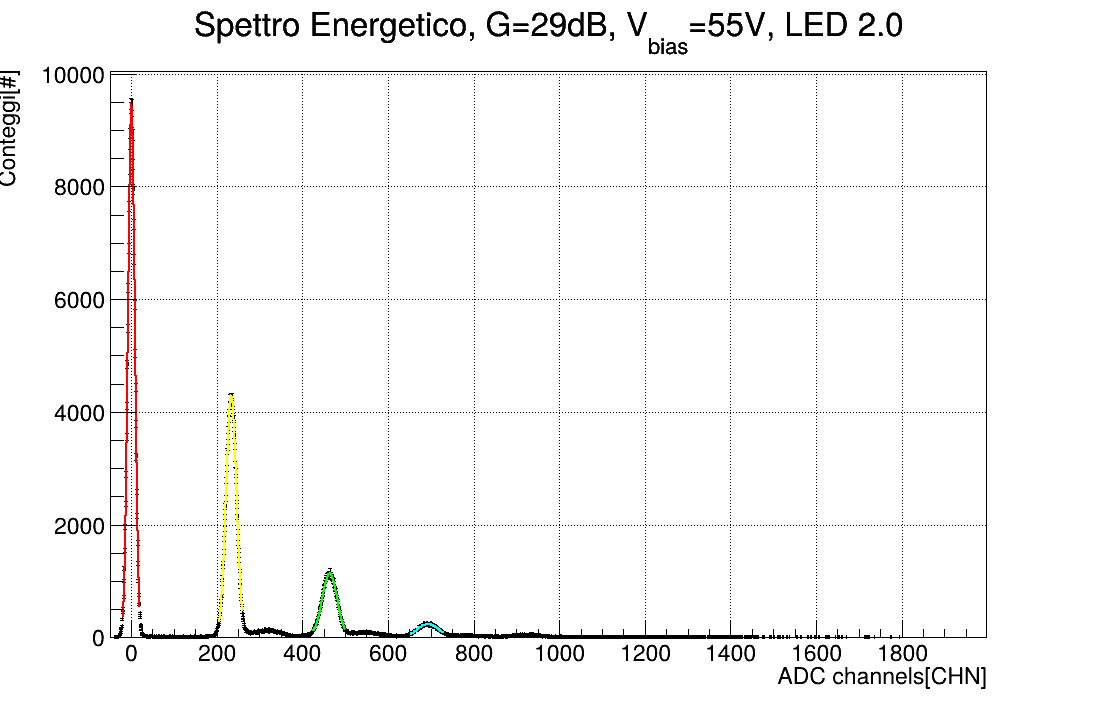
\includegraphics[width=0.99\linewidth]{appendice/i2_0.png}
     
\end{figure}
\begin{figure}[H]
    \centering
    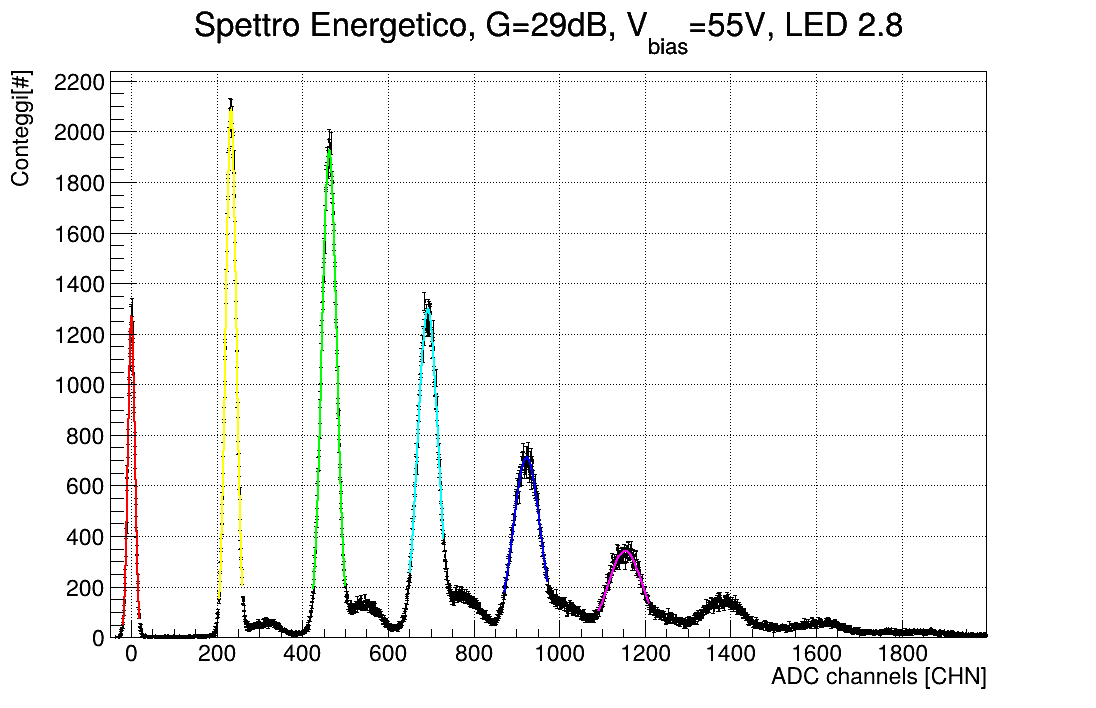
\includegraphics[width=0.99\linewidth]{appendice/i2_8.png}
     
\end{figure}
\end{multicols}

Si riportano gli istogrammi delle aree sottese e i grafici $\sigma^2_N$ vs N.

\begin{multicols}{2}
    \begin{figure}[H]
    \centering
    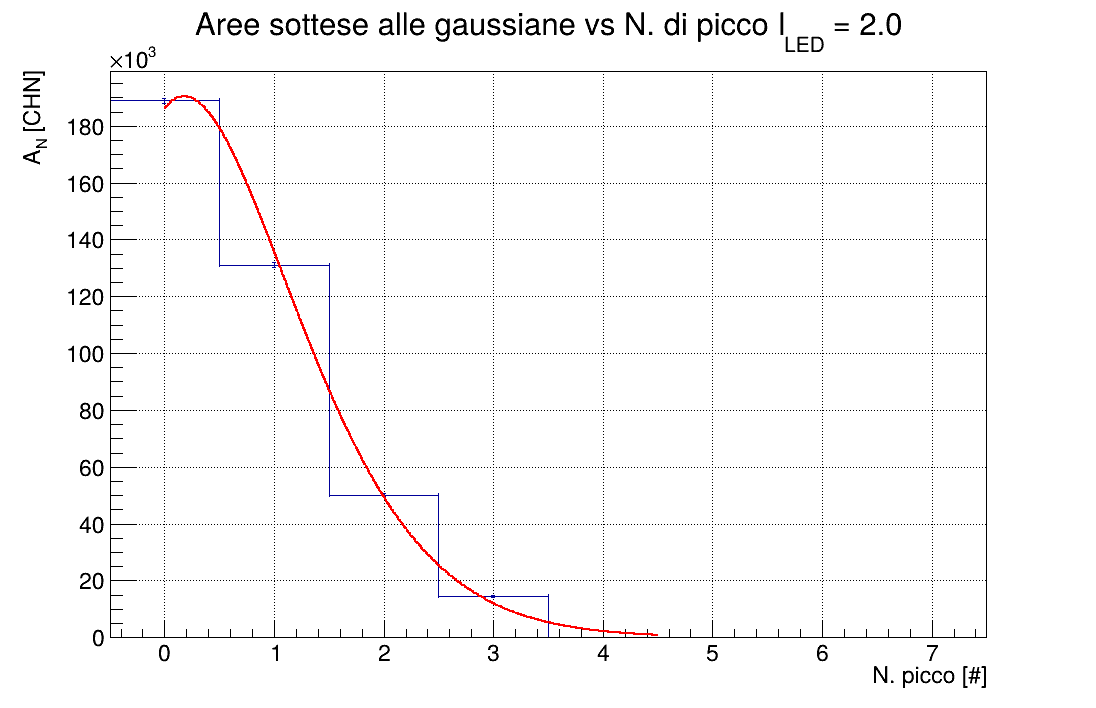
\includegraphics[width=0.99\linewidth]{appendice/pois2_0.png}
    \caption{ \footnotesize $\chi^2 = 93$, d.o.f$=2$.}
     
\end{figure}
\begin{figure}[H]
    \centering
    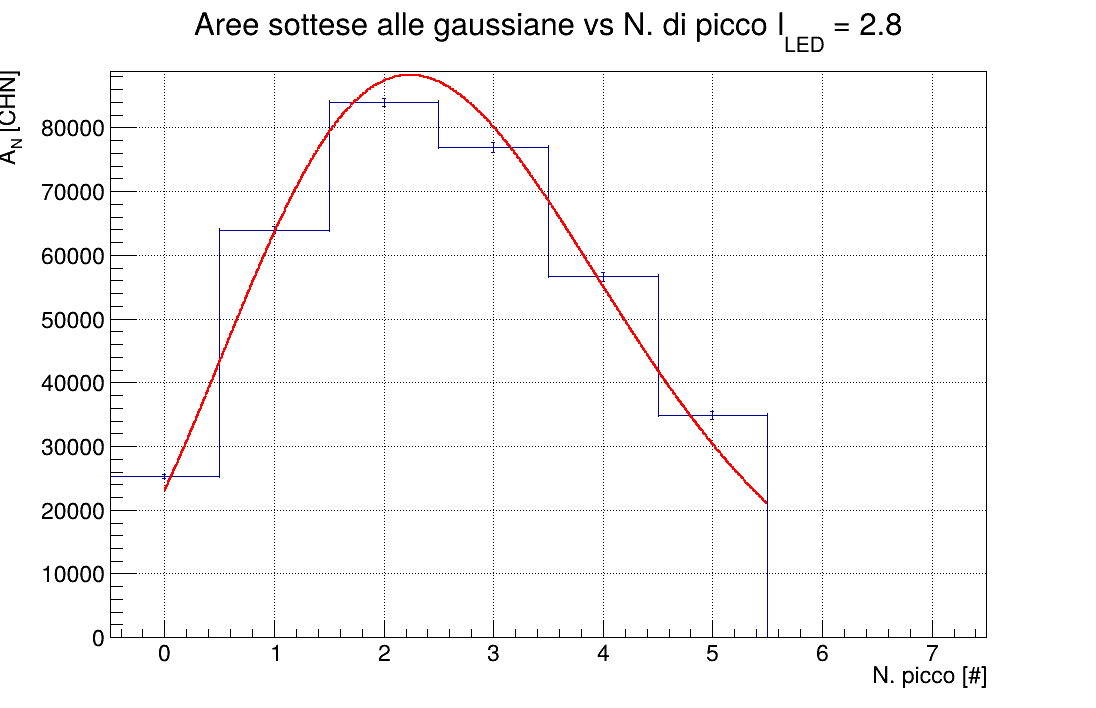
\includegraphics[width=0.99\linewidth]{appendice/pois2_8.png}
    \caption{ \footnotesize $\chi^2 = 143$, d.o.f$=4$.}
     
\end{figure}
\end{multicols}
\begin{multicols}{2}
    \begin{figure}[H]
    \centering
    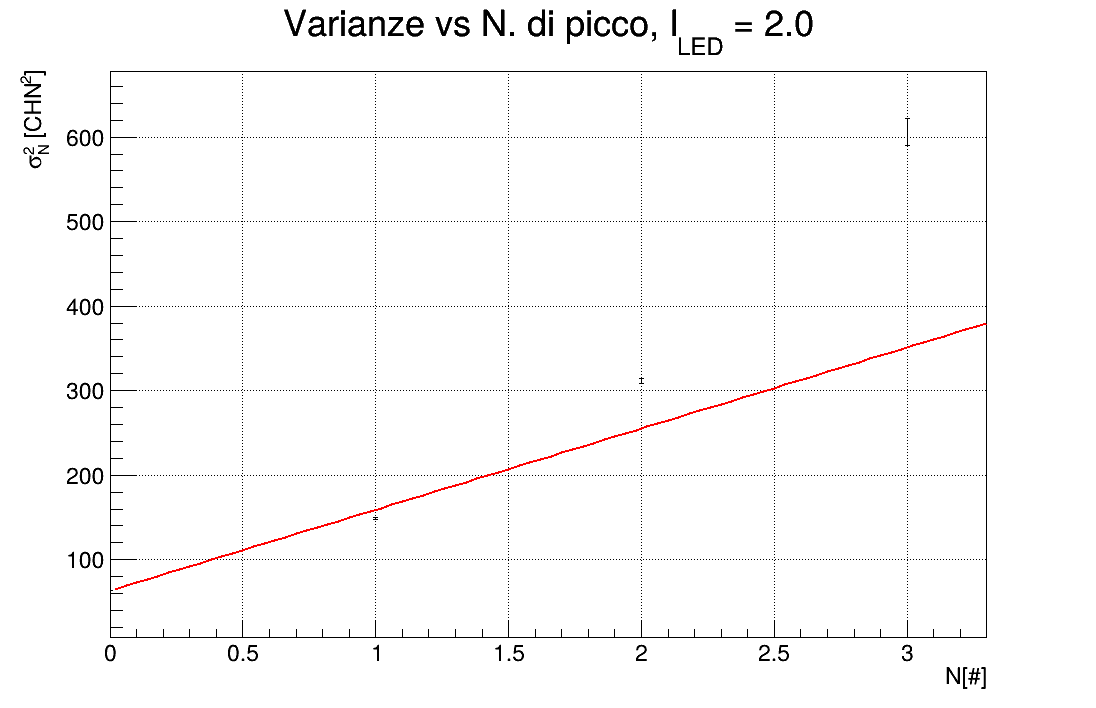
\includegraphics[width=0.99\linewidth]{appendice/sigma2_0.png}
    \caption{ \footnotesize  $\chi^2 = 3379$, d.o.f$=4$.}
     
\end{figure}
\begin{figure}[H]
    \centering
    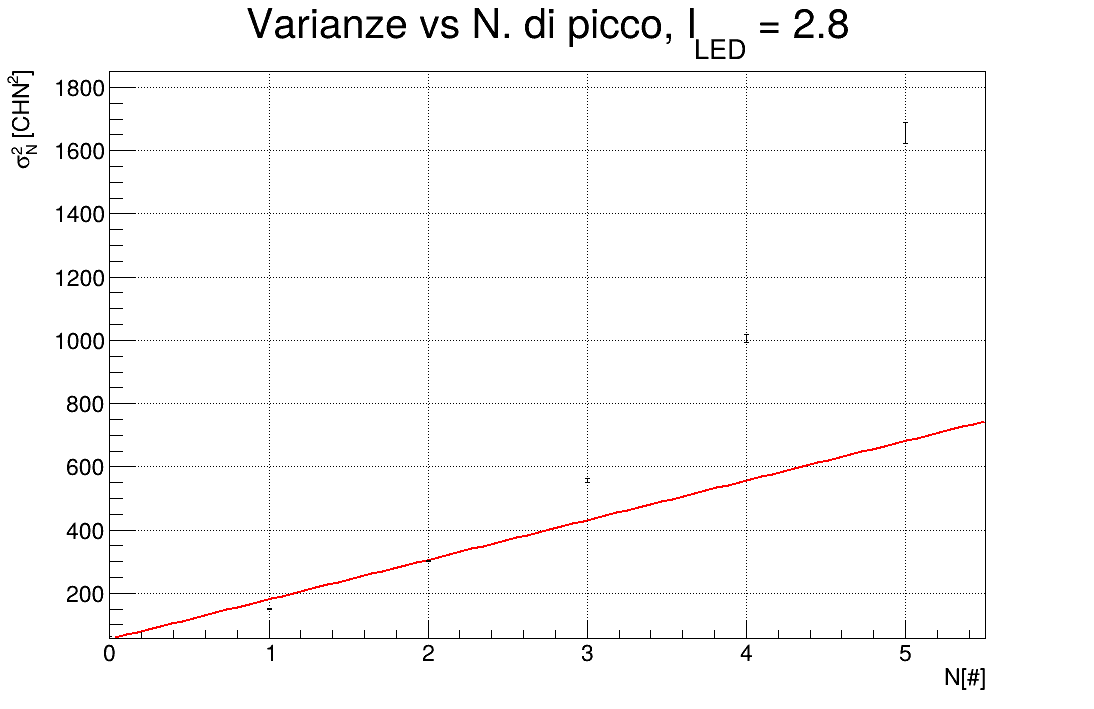
\includegraphics[width=0.99\linewidth]{appendice/sigma2_8.png}
    \caption{ \footnotesize $\chi^2 = 143$, d.o.f$=4$.}
     
\end{figure}
\end{multicols}
\newpage
\subsection{Istogrammi assorbimento $\beta^-$
}
Vengono qui riportati gli istogrammi per l'analisi dell'assorbimento con sorgente di $^{90}Sr$ relativi alla sezione 2.2.1 e 2.2.2 con i relativi fit gaussiani.

\subsubsection{Istogrammi per carta}

\begin{multicols}{2}
    \begin{figure}[H]
    \centering
    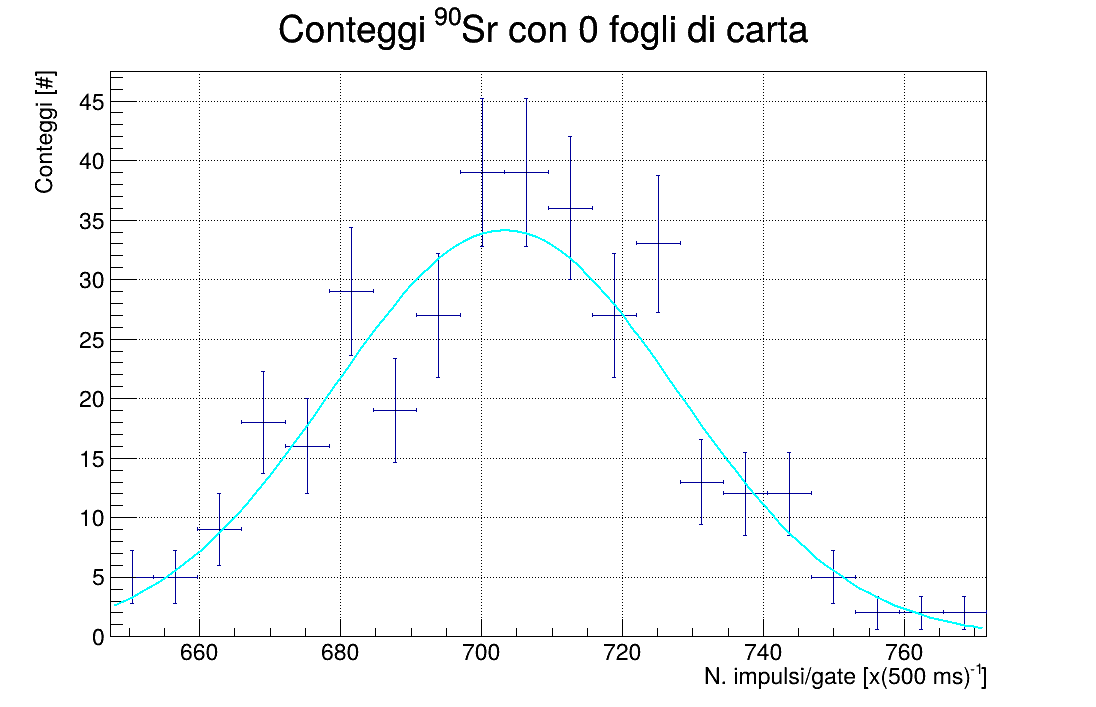
\includegraphics[width=0.99\linewidth]{appendice/carta/c0.png}
    \caption{\footnotesize $\chi^2=17$, d.o.f.$=17$}
     
\end{figure}
\begin{figure}[H]
    \centering
    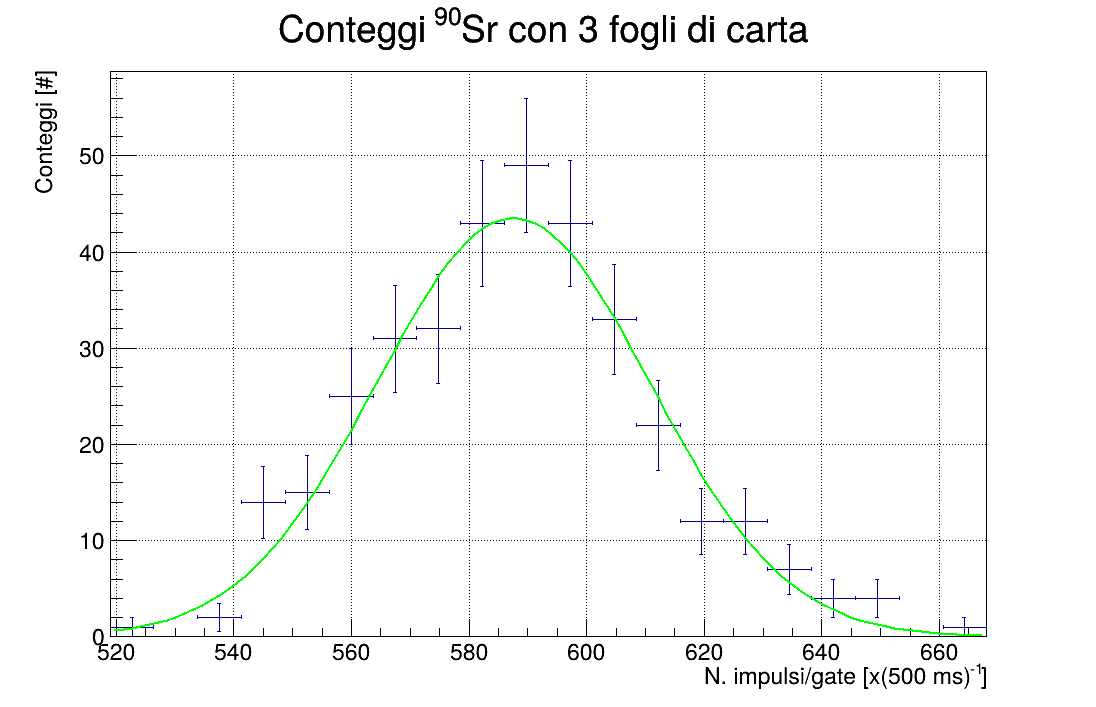
\includegraphics[width=0.99\linewidth]{appendice/carta/c1.png}
    \caption{\footnotesize $\chi^2=13$, d.o.f.$=15$}
     
\end{figure}
\end{multicols}
\begin{multicols}{2}
    \begin{figure}[H]
    \centering
    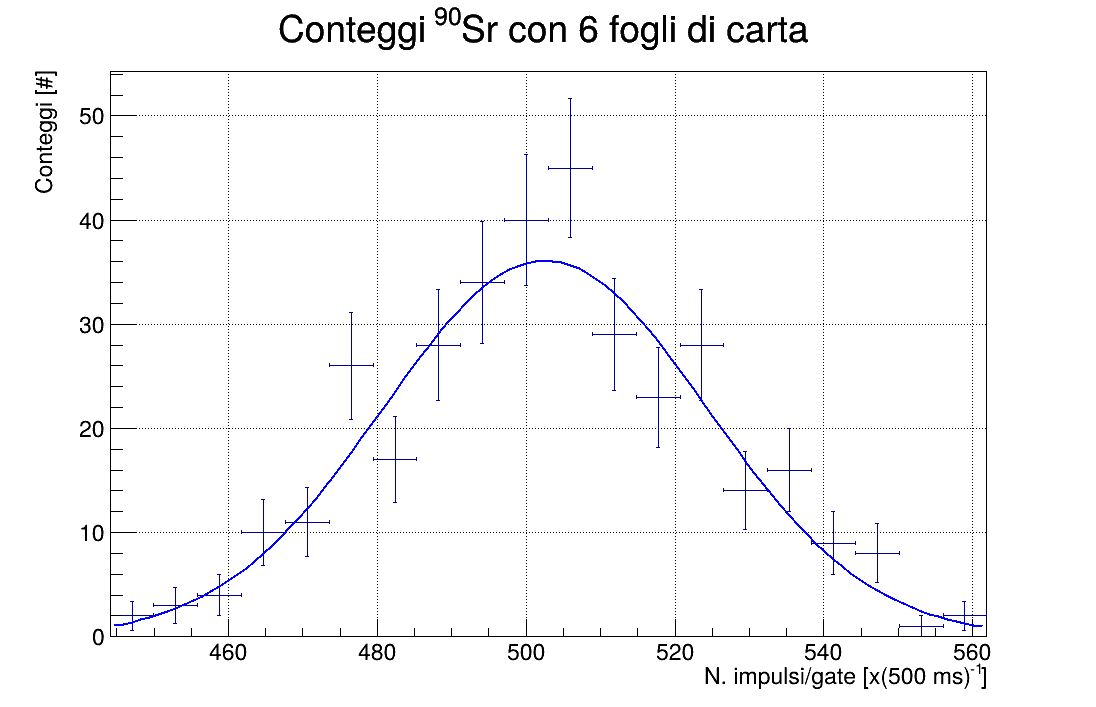
\includegraphics[width=0.99\linewidth]{appendice/carta/c2.png}
    \caption{\footnotesize $\chi^2=17$, d.o.f.$=17$}
     
\end{figure}
\begin{figure}[H]
    \centering
    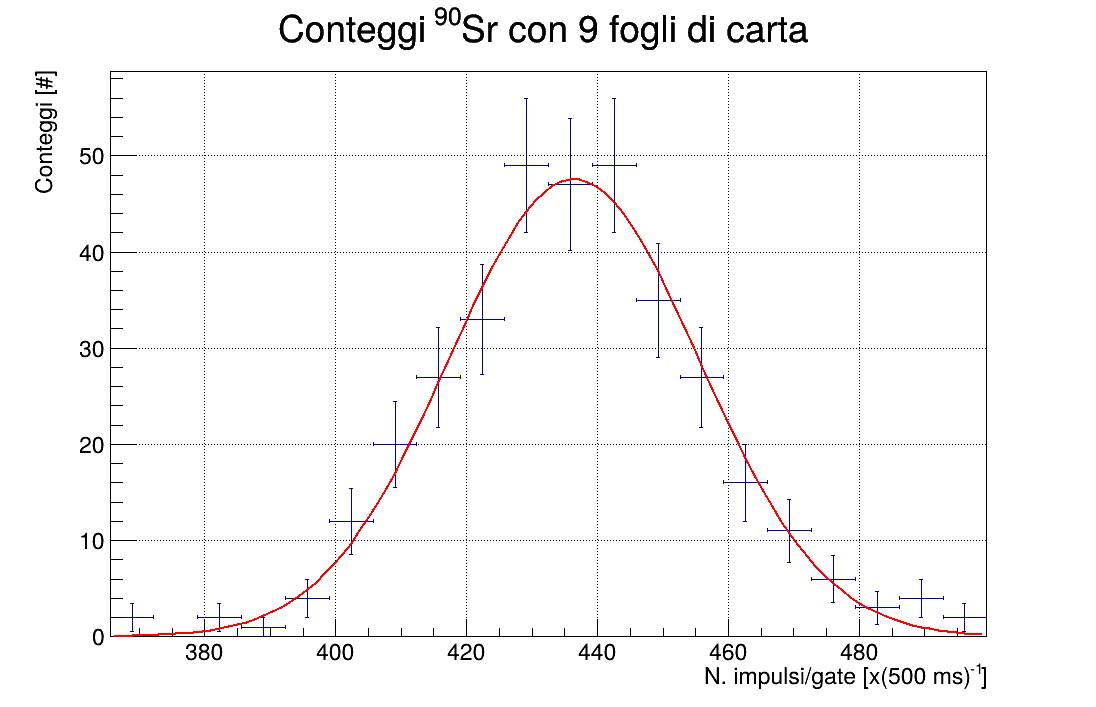
\includegraphics[width=0.99\linewidth]{appendice/carta/c3.png}
    \caption{\footnotesize $\chi^2=10$, d.o.f.$=16$}
     
\end{figure}
\end{multicols}
\begin{multicols}{2}
    \begin{figure}[H]
    \centering
    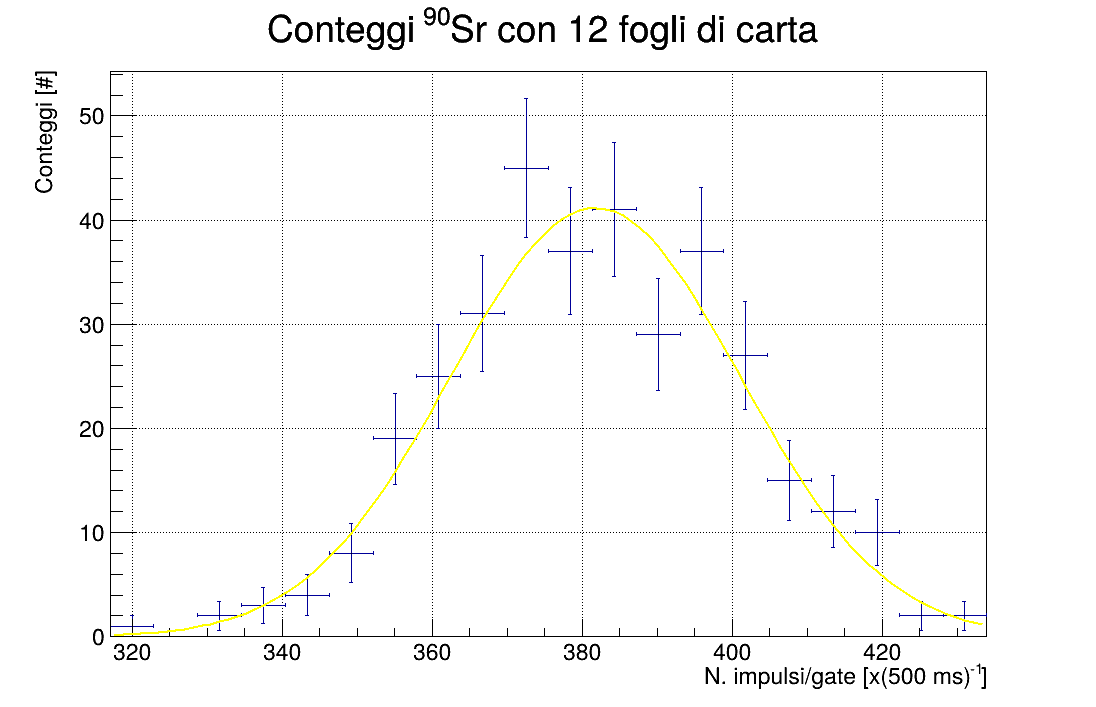
\includegraphics[width=0.99\linewidth]{appendice/carta/c4.png}
    \caption{\footnotesize $\chi^2=11$, d.o.f.$=16$}
     
\end{figure}
\begin{figure}[H]
    \centering
    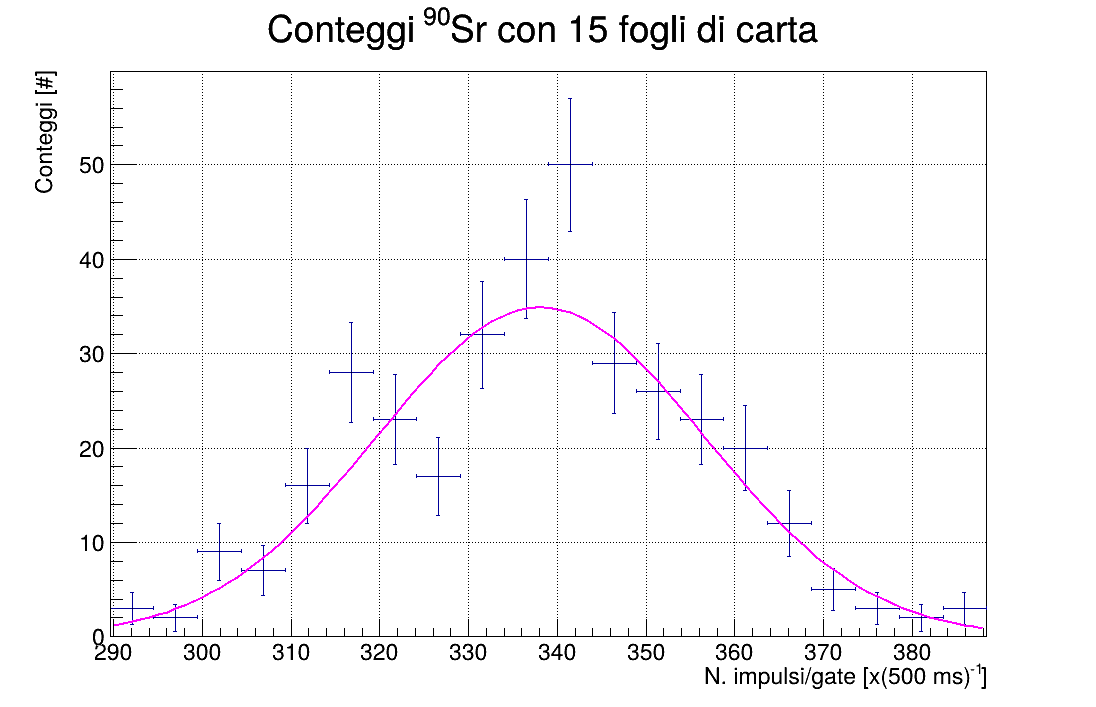
\includegraphics[width=0.99\linewidth]{appendice/carta/c5.png}
    \caption{\footnotesize $\chi^2=25$, d.o.f.$=17$}
     
\end{figure}
\end{multicols}
\newpage
\begin{multicols}{2}
    \begin{figure}[H]
    \centering
    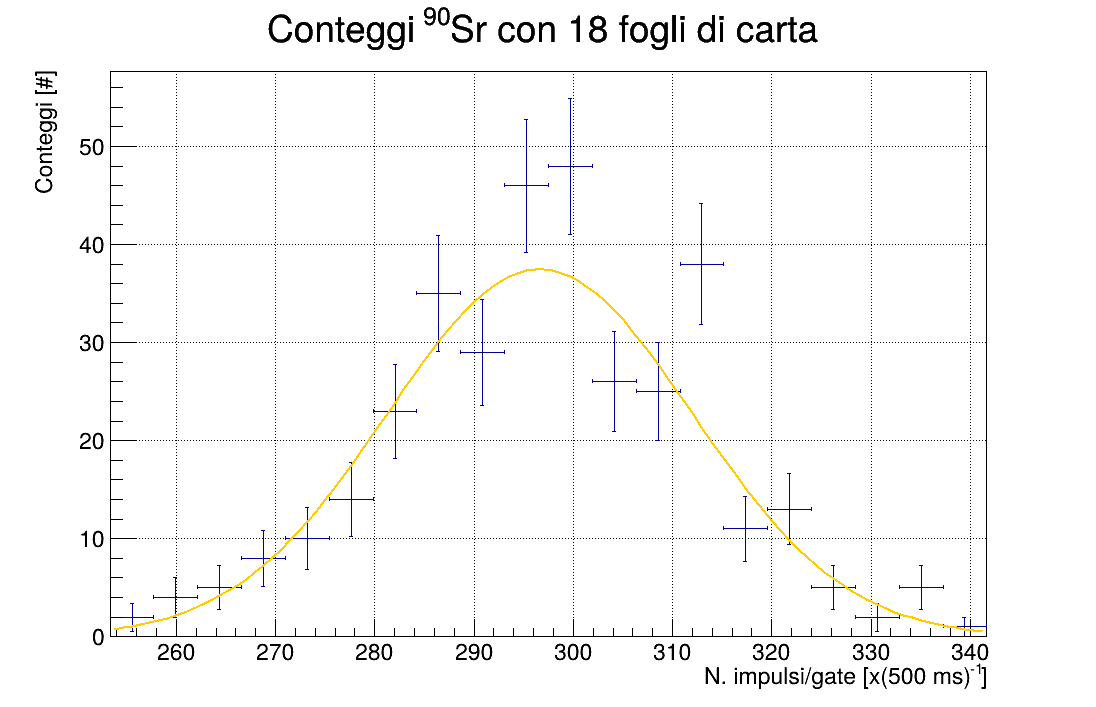
\includegraphics[width=0.99\linewidth]{appendice/carta/c6.png}
    \caption{\footnotesize $\chi^2=24$, d.o.f.$=17$}
     
\end{figure}
\begin{figure}[H]
    \centering
    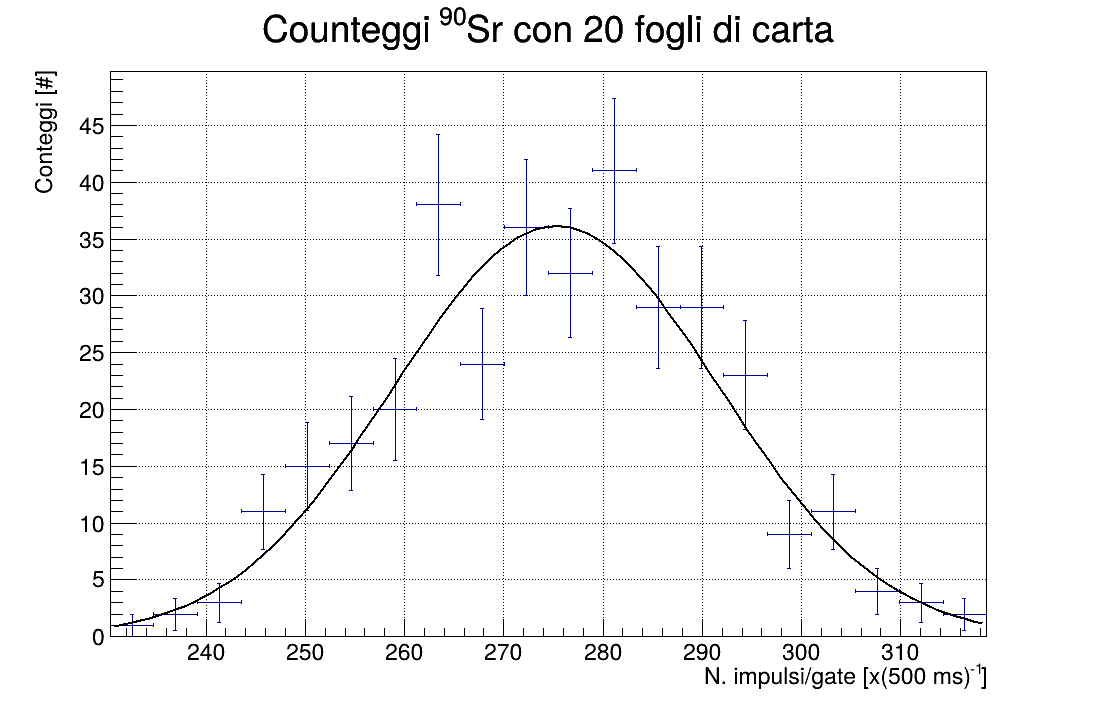
\includegraphics[width=0.99\linewidth]{appendice/carta/c7.png}
    \caption{\footnotesize $\chi^2=15$, d.o.f.$=17$}
     
\end{figure}
\end{multicols}

\subsubsection{Istogrammi per alluminio}

\begin{multicols}{2}
    \begin{figure}[H]
    \centering
    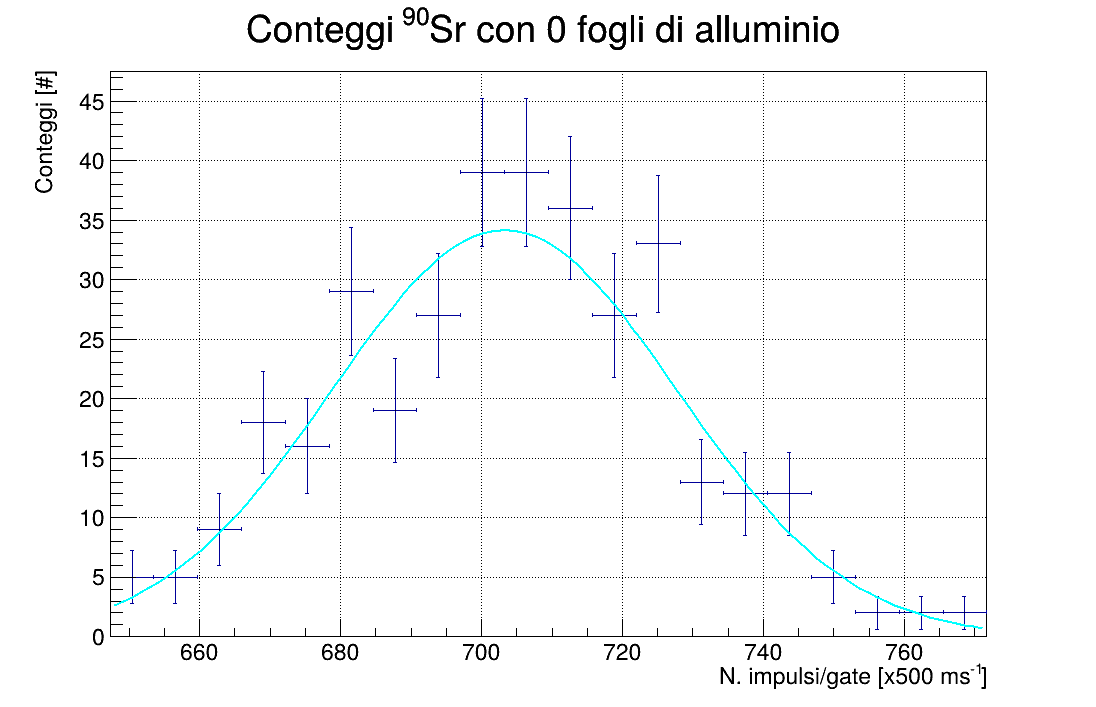
\includegraphics[width=0.99\linewidth]{appendice/alluminio/p0.png}
    \caption{\footnotesize $\chi^2=18$, d.o.f.$=17$}
     
\end{figure}
\begin{figure}[H]
    \centering
    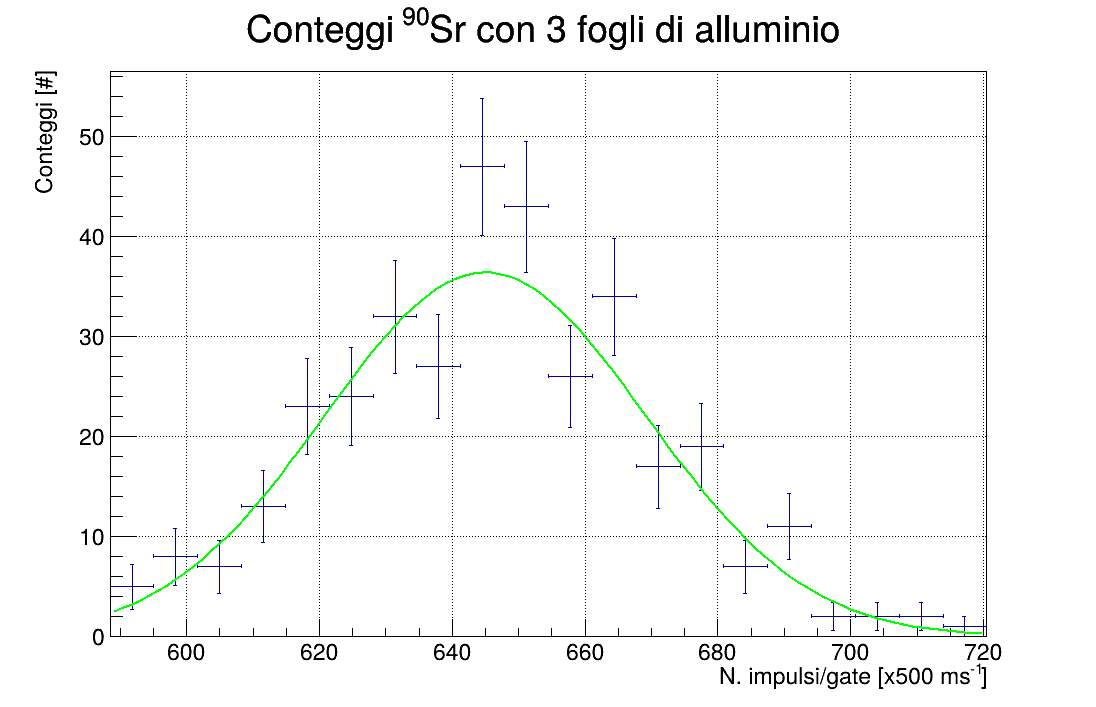
\includegraphics[width=0.99\linewidth]{appendice/alluminio/p1.png}
    \caption{\footnotesize $\chi^2=19$, d.o.f.$=17$}
     
\end{figure}
\end{multicols}
\begin{multicols}{2}
    \begin{figure}[H]
    \centering
    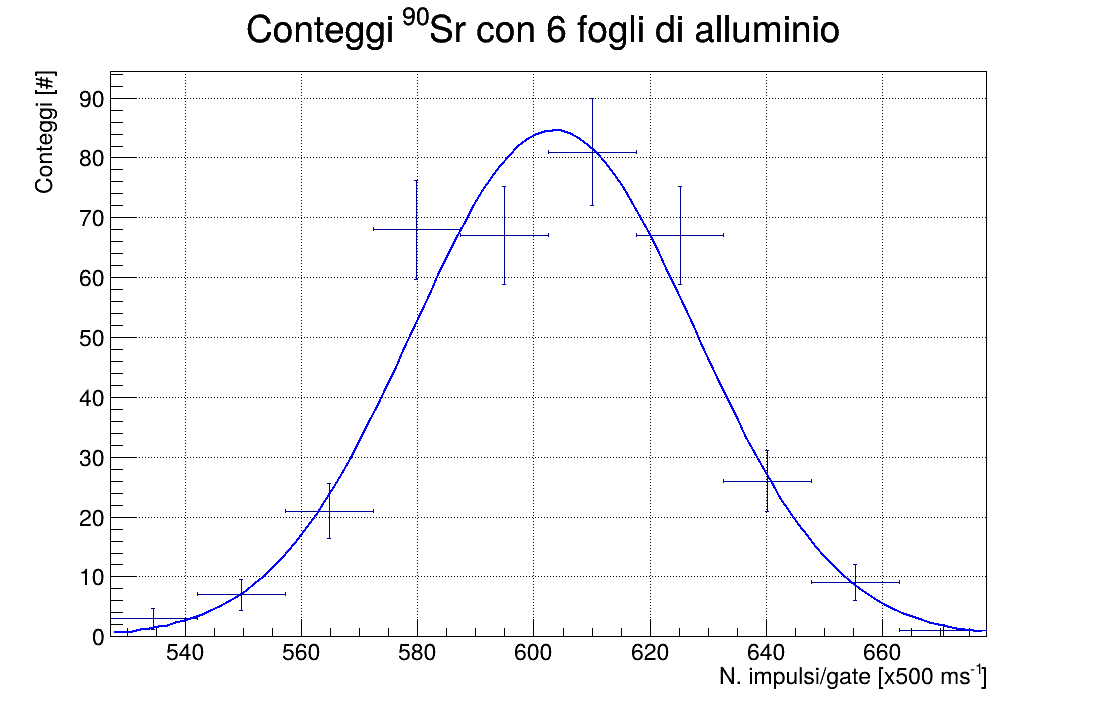
\includegraphics[width=0.99\linewidth]{appendice/alluminio/p2.png}
    \caption{\footnotesize $\chi^2=9$, d.o.f.$=7$}
     
\end{figure}
\begin{figure}[H]
    \centering
    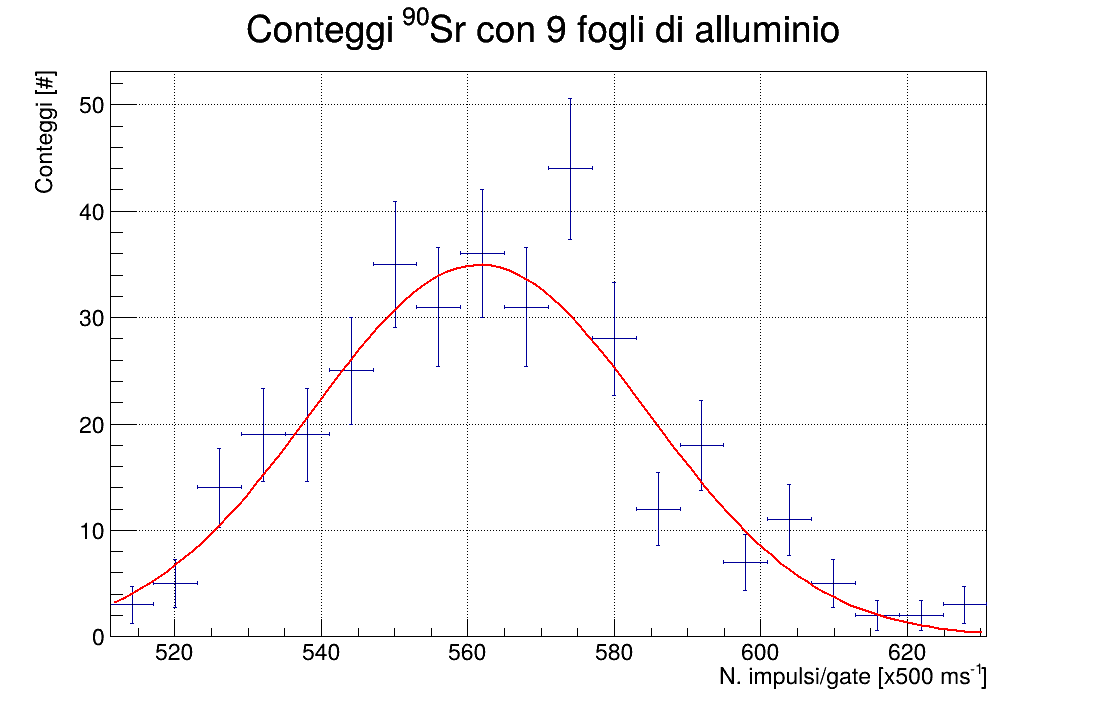
\includegraphics[width=0.99\linewidth]{appendice/alluminio/p3.png}
    \caption{\footnotesize $\chi^2=20$, d.o.f.$=17$}
     
\end{figure}
\end{multicols}
\newpage
\begin{multicols}{2}
    \begin{figure}[H]
    \centering
    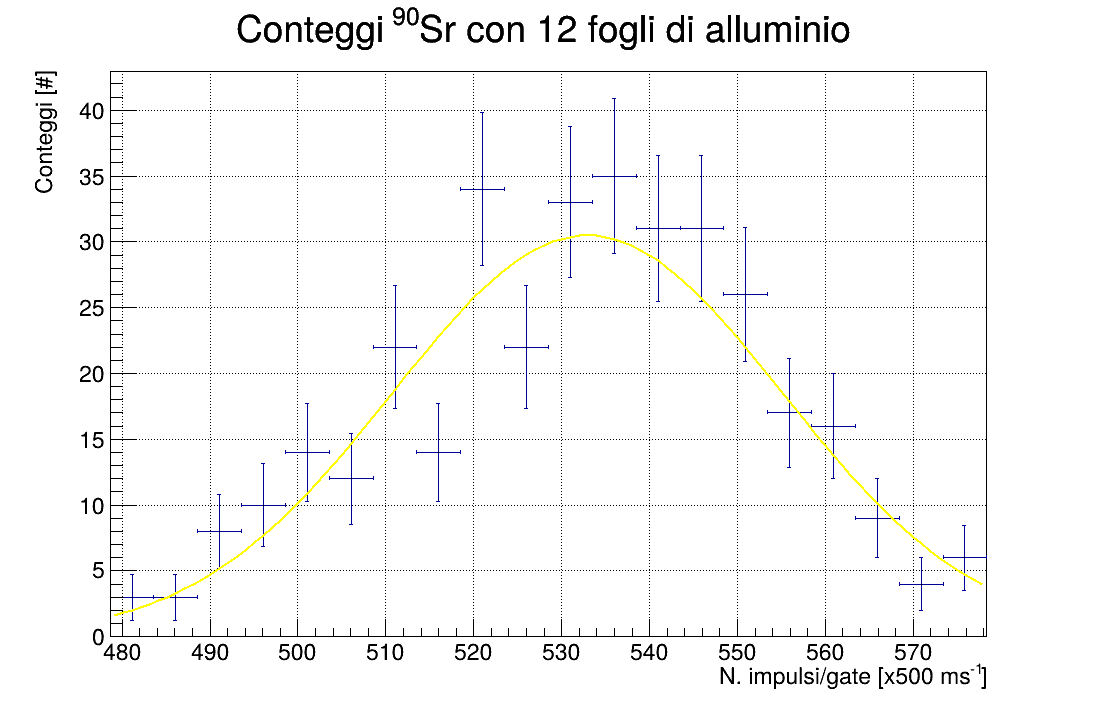
\includegraphics[width=0.99\linewidth]{appendice/alluminio/p4.png}
    \caption{\footnotesize $\chi^2=19$, d.o.f.$=17$}
     
\end{figure}
\begin{figure}[H]
    \centering
    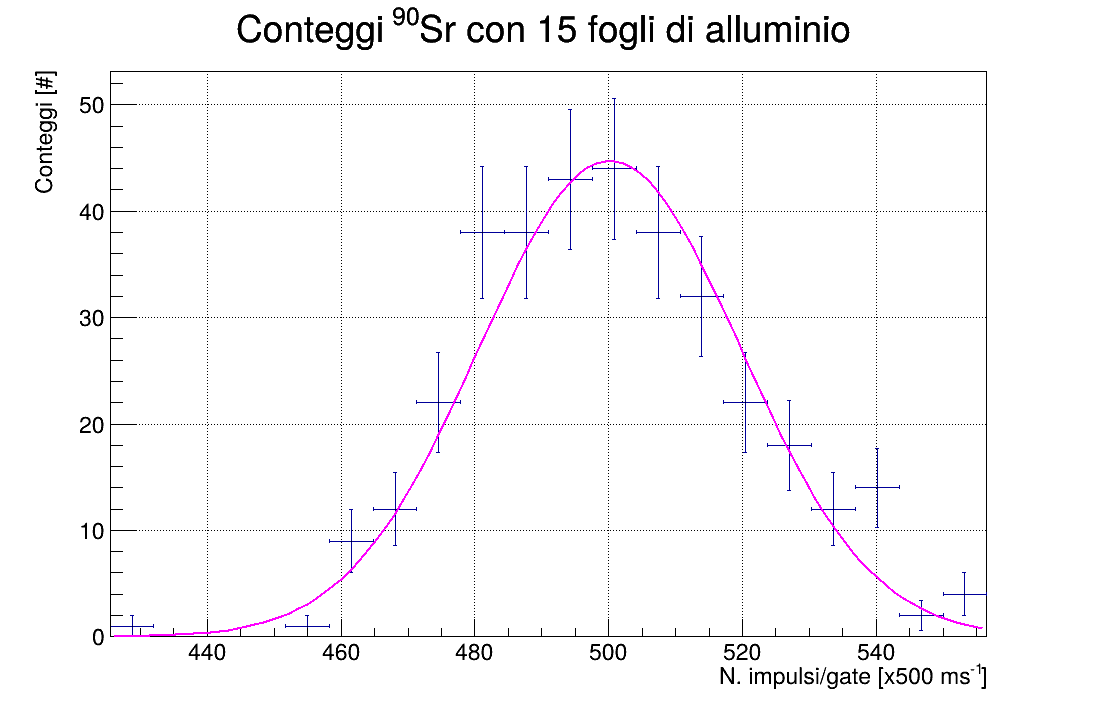
\includegraphics[width=0.99\linewidth]{appendice/alluminio/p5.png}
    \caption{\footnotesize $\chi^2=18$, d.o.f.$=14$}
     
\end{figure}
\end{multicols}


\begin{multicols}{2}
    \begin{figure}[H]
    \centering
    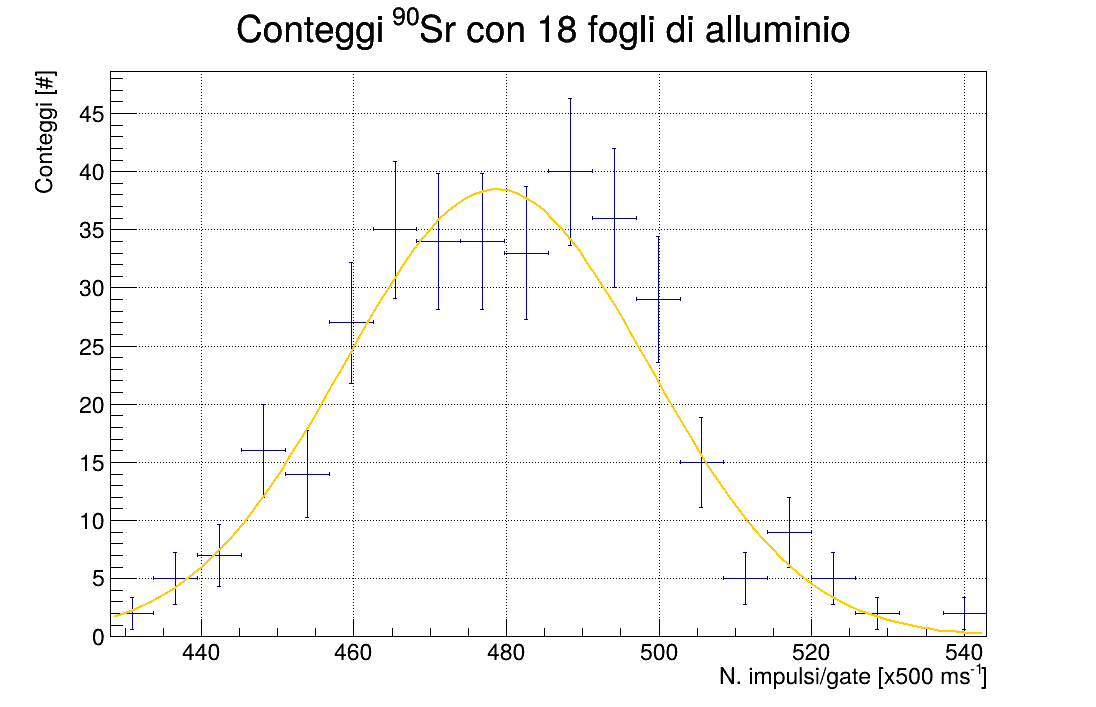
\includegraphics[width=0.99\linewidth]{appendice/alluminio/p6.png}
    \caption{\footnotesize $\chi^2=17$, d.o.f.$=16$}
     
\end{figure}
\begin{figure}[H]
    \centering
    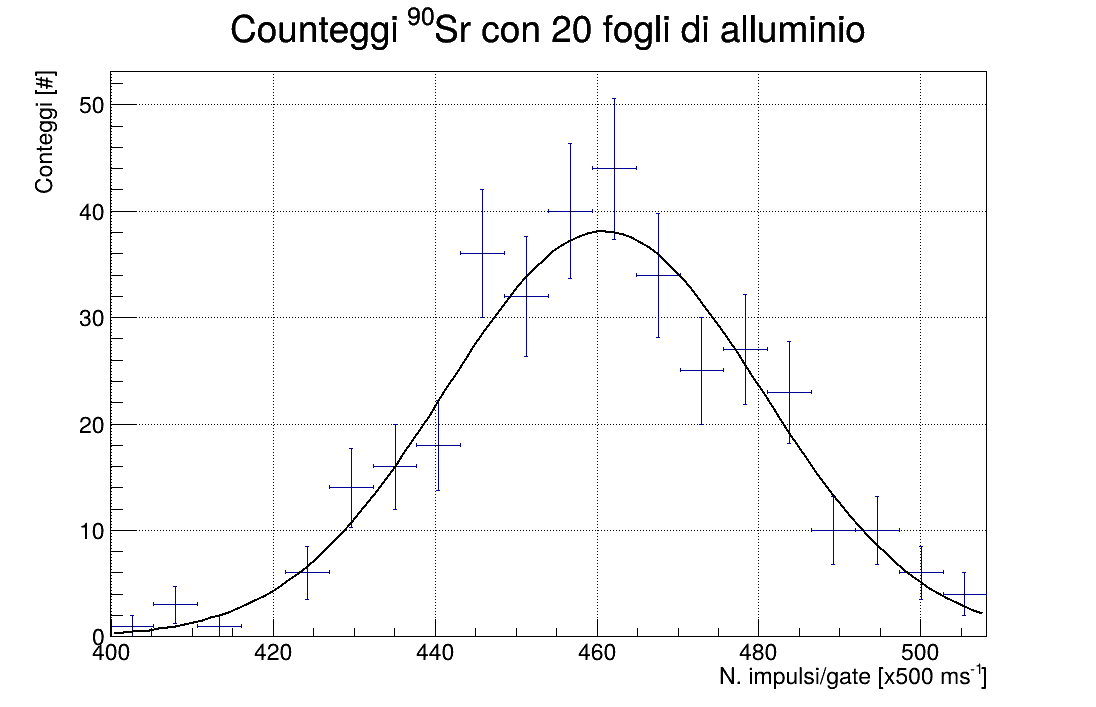
\includegraphics[width=0.99\linewidth]{appendice/alluminio/p7.png}
    \caption{\footnotesize $\chi^2=11$, d.o.f.$=16$}
     
\end{figure}
\end{multicols}

\subsection{Picco di conversione interna del ${}^{137}$Cs}

Si riportano i parametri del fit del picco di conversione interna: i pedici $1$ sono riferiti all'andamento decrescente dello spettro, mentre quelli $2$ al picco di conversione interna.
$$y = N_1 \exp\left\{-\frac{(x-\mu_1)^2}{2\sigma_1^2}\right\} + N_2 \exp\left\{-\frac{(x-\mu_2)^2}{2\sigma_2^2}\right\}$$

\begin{table}[H]
    \centering
    \begin{tabular}{|c|c|c|c|c|c|c|c|}
    \hline
    $\mathbf{N_1 [\#]}$ & $\mathbf{\mu_1}$\textbf{[CHN]} & $\mathbf{\sigma_1}$\textbf{[CHN]} &
    $\mathbf{N_2 [\#]}$ & $\mathbf{\mu_2}$\textbf{[CHN]} & $\mathbf{\sigma_2}$\textbf{[CHN]} & $\mathbf{\chi^2}$ & \textbf{d.o.f.}\\
    \hline
    $9700\pm1600$ & $-3300\pm1200$ & $8400\pm300$ & $719\pm6$ & $19700\pm30$ & $251\pm20$ & 325 & 286 \\
    \hline
    \end{tabular}
\end{table}
\newpage
\subsection{Stima di $\langle \Delta_{pp}\rangle$ per lo spettro del ${}^{137}$Cs}

Si riportano qui i valori dei picchi della sezione 2.3.3, le loro incertezze e le stime di $\Delta_{pp}$.

\begin{table}[H]
    \centering
    \begin{tabular}{|c|c|c|c|c|}
        \hline
        
        \textbf{N. picco} & \textbf{$\mathbf{\chi^2}$ fit} & \textbf{d.o.f.} &$\mathbf{(p_i\pm\sigma_{p,i})\cdot10}$\textbf{[CHN]} & $\mathbf{\Delta_{pp}\cdot10}$\textbf{[CHN]} \\ \hline
        1   & 8 & 8 & $143\pm5$    & \textbf{X} \\ \hline
        2   & 4 & 5 & $160\pm4$    & $17\pm6$ \\ \hline        
        3   & 11 & 6 & $178\pm5$  & $17\pm7$ \\ \hline
        4   & 16 & 8 & $195\pm6$   & $17\pm7$ \\ \hline
        5   & 13 & 9 & $213\pm6$ & $18\pm8$ \\ \hline
        6   & 9 & 9 & $230\pm 7$ & $17\pm9$ \\ \hline
        7   & 11 & 7 & $248\pm6$ & $18\pm9$ \\ \hline
        8   & 6 & 7 & $266\pm6$ & $17\pm9$ \\ \hline
        9   & 10 & 8 & $283\pm7$ & $17\pm10$ \\ \hline
        10   & 5 & 7 & $300\pm7$ & $17\pm10$ \\ \hline
    \end{tabular}
    \caption{\footnotesize Coordinate dei picchi, parametri dei fit e stime di $\Delta_{pp}$ utilizzate per il calcolo di $\langle\Delta_{pp}\rangle$ .}
    \label{tab:zoomcs}   
\end{table}


%\bibliographystyle{plain}
%\newpage
%\bibliography{references}

\end{document}
